\documentclass{scrbook}

\usepackage{graphicx}
\usepackage{hyperref}

% TODO: Figure out a better name for this environment
\newenvironment{thought}
{\begin{itshape}}
{\end{itshape}}
\newcommand{\aside}[1]{\textit{#1}}

\title{Kicks}
\author{Una}
\begin{document}
\maketitle
\tableofcontents
\newpage
\chapter{Models Wanted}

``Models Wanted -- No Experience Necessary -- Local ladies needed to sit for artist. No nudity,
but an open mind is required! Top pay.''

I remember the day it all started. I pondered the classified ad for a while before I sent it
to Kicks. Kicks is a local newspaper, catering to the 18-25 year old crowd. It got started by
some enthusiastic journalism students at the college. After its first year, it became extremely
popular. So popular that it was able to sell advertising space so easily that it could actually
circulate for free. After these students graduated, they kept it going, as it became quite
lucrative for them, despite the fact that it is distributed for free. Almost every college
student has their set place where they pick up their copy every week.

The paper has quite a personals/classified ad section, where one can usually find anything
from someone selling a mountain bike to lesbian biker women looking for a third.

It hadn't been long since I'd settled near town before I got my idea. I've always loved the
idea of casting women, and sketching or painting them afterwards.

Oh, I've had girlfriends in the past who would have been more than willing to participate in
almost anything I asked them to. I've had a lifetime of ``yes-men'' and ``yes-women'' who did
everything they could to make me happy. Of course, they were only doing it because my family was
wealthy. They would gladly have participated in my art, not for the sake of my art, but for the
sake of my money. While most of the time, I would have preferred to have been alone, I put up
with these people to keep my father happy. He worked so hard to make us rich, he wanted us to
experience every benefit that money could bring. I played along, mostly out of respect for him.
I even got to go to a great school to pursue my art studies. The only casting I ever got to do
was on myself, hoping for the day when I could cast a beautiful woman.

After the death of my parents, I decided to change things around a bit. I sold all the
houses except the one in Florida, (That was my dad's favorite house) and all of the other
trappings that come with money. I invested the money, and took off in an old muscle car (OK, so
I kept one indulgence) to see America. I roamed around the country for a few years, sometimes
staying in a place for a few months, sometimes, just passing through. There is a whole other
America out on the country roads, and I loved experiencing it.

I came to this town about a month ago. One day, I saw two coeds going to class. One of them
was on crutches, with a pink long leg cast. She was very pretty, and I couldn't help but sneak a
good stare at her, crutching along, chatting with her friend. At that point, inspiration hit the
way it always does- Suddenly, completely, and without warning. I knew what I wanted to do.

I found an old Victorian style house in town that was for rent. It was perfect- it would be
a nice place to live, and an excellent studio. I went around the antique malls and bought some
very nice furniture for the downstairs. It would be the perfect backdrop for photos and drawings
of casted women.

I chose one of the downstairs rooms to serve as the casting area. A couple of quick phone
calls netted me all of the items I could imagine I might need. I acquired a medical exam table,
a few sets of crutches, to accommodate differing heights, and a wheelchair. I made sure that the
wheelchair had a reclining back, just in case I decided to do a hip spica, and had to move a
woman so casted.

I also found a medical supply house that would sell casting supplies to me. I was a bit
nervous about asking, but apparently they were more interested in making the sale than the
reason for my buying. I purchased padding, stockinette, and plaster, all in varying widths. I
also bought quite a supply of fiberglass bandages, in varying widths and colors. I didn't want
to have to plan ahead on anything. I wanted to be ready for any sort of cast that I decided to
do. I took the supplies to the casting area, and stocked up my cart that I had bought to work
from.

My last step was to call the paper about placing the ad. I got the prices and deadline
schedule. I thought for a while about the wording, then wrote it out, and dropped it in the
mail.

With the ad in the mail, the wheels were in motion. That left me only to wait for the first
call.

\chapter{Adrienne}
My advertisement seeking models came out with the paper on Wednesday. Thursday morning at a
quarter past nine, the phone rang:

``Hello, my name is Adrienne. I'm interested in the modeling job you advertised in Kicks.''

She turned out to be a student at the university, which came as no surprise, of course. She
didn't have any modeling experience, but I wasn't asking for that, anyway. She asked about the
nature of the modeling, given the fact that I had stated that ``An open mind is necessary'' in
my ad. I told her it would be best to discuss it at an interview, and we agreed to meet at the
studio later that day.

When she arrived, I was quite pleased. She had light brown hair, nice features, very
attractive. She would definitely make an excellent cast model, no doubt about it. I hoped that
she would agree to sit for me.

I invited her into the parlor to sit, and introduced myself.

``I'm Harlan Quinn and I am what you could call a fetish artist.''

I couldn't help but notice the bit of surprise that crossed her face.

``Oh, you mean like leather and latex? That sort of thing?''

``Well, Adrienne, those are certainly fetishes, but the one I work in is a bit off of the
beaten path, even as fetishes go. What you will be doing, if you take this job,'' I paused- I
almost felt like I was watching someone else do this, ``is this: You will come to this studio in
the afternoon. You will be placed in a plaster or fiberglass cast, or possibly more than one.
Afterwards, I will take some photographs of you, and then sketch you. After the sketch is done,
I will remove the cast or casts, and will pay you three hundred dollars.''

She looked shocked. ``You mean a cast like for a broken arm or broken leg or something?''

``Yes, just like one a doctor would give you for a broken arm or broken leg- made the same
way, with the same materials. It's an odd fetish, but there are people who like it. Have you
ever worn a cast before?'' She said that she had not, but that she'd had a friend in eighth
grade who had broken a leg, and that the cast had looked to her like quite an ordeal.

She asked questions about the application, and removal. I could tell she was interested. I
told her if she would feel more comfortable having a friend present during this, that she was
more than welcome to bring one along. Male, female- it didn't matter to me, as long as she were
comfortable.

``How will you get the cast off?''

``I use the same tools for removal that a doctor would. They are quick, safe, and painless''

``OK, I think I can do this,'' she said. ``What sort of cast would I wear?''

I hadn't been sure, but I knew I had to reply quickly- if I sounded the least bit unsure of
myself, it might make her uneasy. Leg casts are definitely some of my favorites, so I'll start
there.

``Well, Adrienne, I think I'd like to place your legs in casts, both of them. One will stop
below the knee, and the other will go all the way to your hip. If you think you can do that, we
can set up a day for it.''

She thought for a few moments, and then shrugged- ``Sure- I'll do it! When do you want to?''

I asked her when her class schedule allowed her a free afternoon and evening. ``How about
tomorrow?'' she said. I asked if she could be at the studio at three and she agreed.

``What should I wear? Does it matter?''

``Well, wear whatever you like on the way here. Since this art is fetish driven, you'll need
to have something fairly erotic to wear for the sitting. Bring a swimsuit if you have one, and
some attractive lingerie if you have that. Nothing too revealing, though- the ad promised no
nudity, and that promise will be kept.''

She got up, said ``See you tomorrow at three!'' turned and left.

After she left, I sat there, almost dumbfounded. Hard to believe, but I was actually going
to get to cast a woman. I've wanted to all my life, but never have, and now it's going to
happen! I lit a cigarette, and sipped my soda, as I contemplated the final preparations.

I went to the studio, and started loading the supply cart. I debated on whether to use
plaster or fiberglass. I have practiced with both, making casts on myself, so I could do either
one and make a nice looking cast with no problems. I looked through my cache of supplies.
Anything was possible, really. I had enough casting supplies on hand to keep a big city hospital
stocked for a couple of weeks, probably: Stockinette, padding, plaster and fiberglass in all
sizes and colors.

I decided to cast Adrienne in plaster, as the first casts I remember seeing as a child were
all done in plaster. So, to the cart, I added 12 rolls of 4 inch plaster, and 6 rolls of 6 inch
plaster, in addition to several rolls of 4 inch padding, and a roll of 4 inch stockinette.

Adrienne arrived at about ten minutes past three, carrying an overnight bag.

``Sorry I'm late, I hope it's OK.''

``No problem, come on in,''

She apologized again, saying she was trying to talk her roommate into coming along, but with
no luck. ``But,'' she added, ``you look pretty honest and harmless, so I just gave her the
address here, and came alone.''

``That was a smart thing to do,'' I told her. ``I applaud you for your caution. I'd never
hurt anyone, but you barely know me. To you, I'm just a guy with a weird turn-on. Would you like
a soda?''

I got a soda for each of us, and asked her to come with me. I led her to the room I had set
up as a casting room. She looked around, taking it in, the table, the small footstools I had
gotten to use as props for casted legs, the cart of supplies, and the crutches and wheelchair in
the corner.

``Will I be needing those?'' she asked, pointing in the direction of the crutches and chair.

``We'll use the wheelchair to get you to the parlor when the casts have set,'' I told her.

She started poking through the supplies a bit, out of curiosity.

``Let me show you the choices of what I brought to wear,'' She said opening the bag she was
carrying. She produced a one-piece swimsuit that wasn't bad, but it didn't seem quite right to
me. She then brought out a satin nightgown and a babydoll style teddy.

``Of course, there's always these'' and as she said this, she raised her sweatshirt to show
a blue bra, then unfastened her Levis and pulled them down far enough to show the matching
underwear. That was what I was looking for.

``Let's just go with what you have on under your clothes right now, and we can start
whenever you're ready'' She took off her shoes and socks, slipped her jeans and sweatshirt off,
folded them neatly, and placed them in the corner. She then hopped up on the table and said
``I'm ready whenever you are''

I took an envelope from the cart, and opened it. I removed four one hundred dollar bills
from it, showed them to her, then replaced them in the envelope.

``I know I told you three hundred dollars, but I got the OK for an extra hundred since there
was an extra cast involved.''

``Great! I appreciate that!''

I then placed the envelope with her clothes. ``There. I wanted you to see the cash before
you see the casts'' She smiled and nodded. I could tell she was still a bit nervous.

I rolled the cart to the table. I took the bucket, excused myself, and went to fill it with
warm water. Adrienne was sipping her soda when I got back.

``OK, here we go,'' I told her, as I took the roll of 4 inch stockinette from the cart. She
said nothing as I did this.

I slipped the stockinette over her left leg, to just past the knee, explaining that it
served as a base for the cast, and kept the padding from itching. I cut it off just past the
toes, and smoothed out the wrinkles. Propping her left leg on the rest I had made, I then moved
to the right leg, where I brought it all the way up to her hip, being very careful to do it in a
professional manner. I then cut it off just below the toes, then propped it on the other rest.

Next, I brought out a roll of 4 inch padding. ``Adrienne, this is the padding. It gives a
bit of comfort to the cast, and keeps the plaster from directly contacting your skin.'' Again
she only nodded. I hoped that her nerves would be a bit more calm when she actually sat for me,
as I would prefer a smile on her face.

Since she wasn't going to be walking on these casts, I didn't think that heavily padding
them was necessary. With the left leg, I started at the toes, and overlapped the previous wrap
by one half. This gave her a double thickness of padding, to the knee. Next, the right leg,
wrapped the same way, only going much higher, stopping at the top of the thigh.

There she was, stockinette and padding applied, ready for the plaster. I stepped back and
looked at her and nodded to myself.

``Well, we're ready for the plaster. Are you still OK with this?'' I asked.

``Yes, it's actually sort of fascinating'' she replied. ``You seem to really know what
you're doing with this. Have you done it before?''

``Yes, I have. You're not dealing with a rookie, here.'' I told her with a smile. She smiled
back, and I got back to work.

I started with her left leg. I tore open the first roll of plaster, and dipped it. ``As this
starts to set, you will feel some heat from it, but I promise you it will not get anywhere close
to burning you,'' I told her as I began to wrap her foot.

I started with the ankle, working my way to the toes, then back up past the ankle. The
second roll started at the toes, building thickness, and continued over the ankle. The third
roll started at the knee, and worked down until it met up with the plaster already at her foot.
The fourth and fifth rolls repeated this, until I had a good, strong, thick base. I worked the
plaster in, smoothing it with my hands. The cast was looking great.

``It's starting to get warm on my foot,'' she announced.

``Yes, that's quite normal'' I replied.

I wiped my hands off, took my scissors, and trimmed the padding back to be almost flush with
the plaster. I folded the stockinette back over the cast, and used some of the wet plaster to
hold it in place for the moment. Another roll of plaster, starting at the foot, to anchor the
stockinette and padding, followed by another roll, doing the same thing, only from the top of
the cast. I could feel the heat on my hands as I smoothed out the rapidly setting plaster. The
cast was finished, and it looked great!

``Well, there's one leg done.'' I told her, as I gently placed her foot on the padded stool.
``We'll just set that one here to dry. Are you still OK?''

She smiled and said ``I'm fine- this isn't so bad. And even if it were, I'm being paid very
well for it, so I could deal with it, no problems!''

``OK, then- lets move to the other leg'' I told her. I then turned back to the cart.

I helped her scoot to the edge of the table, allowing me access to her right thigh. I tore
open a roll of six inch plaster, dipped it, and started to work on her long leg cast. I wrapped
the first roll over the knee, building a good strong base there. I didn't try to bring it all
the way up on the first roll. The second and third rolls started at the end of the padding and
worked to just past the knee and back. The fourth roll of six inch started at the top, and
worked down to near the ankle. I then folded over the stockinette and padding at the top, and
anchored it with the fifth roll of six inch, smoothing it out as I went. Then, I moved to four
inch plaster, starting at the shin, and working it to the toes. Four rolls of four inch plaster
later, I was ready to fold over and anchor the stockinette at the toes. I smoothed out the
plaster over the whole cast, and placed that leg on the other stool to let it dry.

``There you are,'' I said. ``We need to just let that dry for about an hour before we can
move you to the other room. It won't be completely dry, but it will be dry enough to move you.
Do you need anything?''

``How about another soda?'' she asked.

I cleaned the plaster from both of us, and we talked for awhile as the plaster dried. After
it seemed pretty well set, I picked her up, and placed her in the wheelchair. I snapped a few
photos of her in the wheelchair. I rolled her into the parlor, where I helped her into a chair.
I snapped a few more photos, and as I was doing so, the inspiration hit me.

``Let's have you lie on the chair, with your legs resting against the backrest.'' I said.
``I think that's how I want to draw you.''

I helped her change positions, and as she relaxed, she lowered one of her bra straps down to
her upper arm.

``There,'' she said, ``That should look pretty good!'' She lowered her head, allowing her
hair to spill down.

Pretty good wasn't an accurate description, she looked fantastic! I snapped a photo of her
this way, then grabbed my tablet and pencils, and went to work furiously.

An hour later, the sketch was done, and I was very pleased with the way it turned out. I
helped her back to a proper sitting position, and showed her the drawing.

``Wow, that's really good- you are very talented! It looks just like me!'' She exclaimed.

``That was the idea.'' I said with a smile. ``OK, are you ready to get out of those?''

I picked her up, placed her back in the wheelchair, and took her back to the table. I lifted
her up onto the table, and got my Stryker saw and bandage scissors. She looked a bit startled by
the saw. ``Don't worry, this saw will not cut you- it is unable to.'' I then turned the saw on,
and placed the oscillating blade against my bare hand to show this. Her relief was obvious on
her face, so I started to work. I cut both casts along both the inside and outside of her legs,
using an in and out motion. I cut small triangular sections from the insides of both ankles and
the right knee, allowing me to turn with the scissors. I then used the scissors to cut the
padding and stockinette along the insides of her legs, and slipped the casts off of her. It was
odd, seeing how the stockinette had imprinted it's pattern on her legs.

``You are all done, Adrienne.'' I told her. ``Thank you for working with me, you were an
excellent model, and I enjoyed the whole experience.''

As she got dressed, she asked ``So, who will be seeing the photos and the drawing? Will they
be seen by a lot of people?''

``Well, that depends upon what my patron wishes to do with them, but I think he keeps them
pretty much to himself.''

``Patron?'' she asked.

``Yes, he's the man who pays for all of this. He loves the sight of casted women, and foots
the bill for all of what I do.''

She shrugged and said ``Well, he pays very well,'' placing the envelope into her bag. ``If
he wants to see more of me, maybe we can work together again. Let me give you my number.'' She
wrote her number down, which I placed in my pocket. ``Thanks again,'' she said, as she turned to
go. As soon as she was gone, I turned and looked at the freshly removed casts on the floor, and
started to clean up. Alone.

\begin{center}
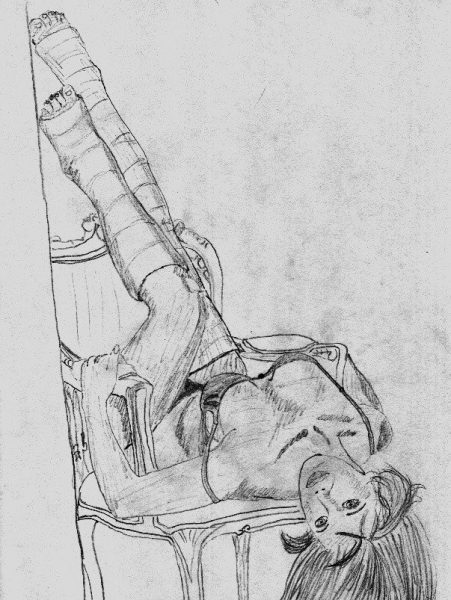
\includegraphics{images/kicks02.jpg}
\end{center}

\chapter{Diane}
After the casting session with Adrienne, there were a few more calls that
first week. These were not as fruitful as the first one had been. Two of the women found the
idea of casts as ``fashion'' too bizarre, and wanted no part of it. The third was a no-show for
the interview. This really did not surprise me. I expected most of the candidates to lose
interest in the job when they found out exactly what it was about. Besides, after the first
casting session, I realized I needed another piece of equipment in the cast room.

The next Saturday, I received another inquiry. After the usual phone info, she agreed to meet me
at the studio in an hour.

When I answered the door, I was impressed with her appearance. She was tall, blonde, very
pretty, and dressed to impress. She wore a white blouse, denim shorts, and sandals. She had a
wonderful smile, with a hint of mischief to it. She introduced herself as Diane, and after I
introduced myself, I led her to the parlor for the interview.

She listened without speaking as I outlined the job I was offering her. When I mentioned the
casts, her eyebrows raised in a quizzical manner. When I had finished, she said

``Well, it's certainly different, but I don't see what could possibly be wrong with it? I broke
my leg my senior year of high school, and I DID notice that I got more attention while I had the
cast on. It hurt like hell when it happened, and the cast was a real pain, but it wouldn't be so
bad for a few hours. What sort of cast would you want me to wear?''

I stood up and asked her to do the same. I walked around her a few times, looking at her and
thinking. Then, I knew what I wanted to do.

``How about a leg cast? One like you had when you broke your leg. It will start at the toes, and
end near your hip.''

She nodded, then asked when I wanted to do it. We discussed her schedule, then settled on Monday
evening. I told her what sort of wardrobe I was looking for, and she seemed fine with that.
After I had told her she was welcome to bring along a friend for safety if she wanted, she left.

Monday afternoon, she arrived on time. She had brought some very nice wardrobe items, and after
we had decided on some lingerie and a beautiful robe, I offered her something to drink, and left
her to change clothes. I went to get her soda and her money.

I tapped on the door when I returned. ``Are you ready?''

``Sure, come on in'' she replied.

She was quite breathtaking, and my heart raced a bit, contemplating what was to come. I placed
her payment with her clothes, and said ``Let's get started'' with a smile.

She hopped up on the table and said ``Which leg?'' I scratched my beard and thought for a
moment. ``Left'' I finally decided. She held out her left leg, and I went to work. I unrolled
some four inch stockinette, and worked it up to her hip. I was very careful to be professional
about the way I did this, I sure didn't want to get a bad reputation, or worse. I cut it off
about 6 inches from her toes, then started at the foot with the four inch padding. Two turns
around the ankle, then out to the toes and back. As soon as I was past the ankle, I tore off the
rest of the roll. That gave her three layers of padding over her foot with a fourth around the
ankle bones and heel. I then started from her thigh with six inch padding, working my way down.
I learned from the first experience that due to the contours of the human leg, the padding goes
on smoother, with less bunching, if you work from the top. One and a half rolls of padding
later, she had two layers over her leg, with an extra around the knee. I taped down the tail of
the last roll, and decided to take a short break before the fiberglass. I checked our sodas, and
offered her a cigarette, She accepted, and I got one for myself, too.

Earlier that day, I had decided to cast Diane in blue fiberglass. I had laid out several rolls
each of four and five inch fiberglass tape. I crushed out my smoke, and went to fill the bucket.

I readied my new contraption. It was a stand about seven feet tall, and it was going to help me
support limbs as I casted them. I had devised two different attachments for it. The first was a
small clamp, that I could attach to a bit of stockinette overhang. The second attachment was a
sling that I could hang from the stand. I had made them so the length would be adjustable. I was
quite proud of my little engineering job, and readied the sling. I placed her leg in the sling,
so that it was supported at the heel. I bent her knee at a 20 degree angle and asked her to hold
it there.

I pulled on my gloves, and asked her if she were ready. She nodded, and I tore open a roll of
five inch fiber. I dipped it, and, starting at the thigh, I rolled the fruity-smelling tape on
her leg, each turn overlapping the previous one by half. The first roll ended just past her
knee, and the second one went right over the first in the same manner. The third roll started
just above the knee, and worked down to the ankle. The fourth roll began at the knee, and got to
the foot before it ended. The cast was already starting to set at the top, so I folded over the
stockinette, and anchored it with another roll of five inch fiberglass, working it down her leg,
finishing the upper portion of the cast.

I waited a few minutes for the bottom layers to set, and when the cast felt solid under her
thigh, I moved the stand to support her leg at that point. This would allow me access to her
foot. Just below her knee, I started with the four inch fiberglass tape. After it had been
wrapped down to the foot, the next roll started at the ankle, went to the toes, and back up to
the shin. Another roll over the top of this one, and the cast was looking thick and strong. I
clipped off the excess stockinette, folded it over, and anchored it down with one final roll of
fiberglass, working it past the ankle.

``It's really starting to get warm'' She said.

I knew it had to be, as I could feel the heat radiating from the outside of the cast.

``I hope it's not too uncomfortable, but it will cool off pretty soon. Are you OK?'' I asked,
pulling off my gloves and tossing them into the trash.

``I'll be fine, it's just a bit warm on my skin.''

I removed her leg from the sling, and placed it on the padded stool to finish drying. I marveled
at how her leg was solid, moving as one unit. I cleaned up my mess as the fiber finished
setting.

``Yes, this is pretty much the same as I remember from the last time. I was surprised at how
fast it got hard.''

``In another ten minutes, it will completely set, as hard as it would get. You could even walk
on it if you wanted to. Let's go ahead and get started with the photos.''

I got the camera, and took a few shots of her on the table. Some of the photos were just of the
cast, while some were full view shots. When I was done, I held up a pair of crutches with one
hand, and pointed to the wheelchair with the other.

``Do you want to walk, or ride?''

``Ride. Those things kill my armpits.''

I lifted her into the wheelchair, and set the leg rest to support her casted leg. I then took
her into the living room, where I took some photos of her in the wheelchair.

``Hey, grab my robe,'' she reminded me. I returned with her robe and helped her to stand up.
After she had put it on, I helped her down onto the couch.

She posed on the couch in several ways, with me getting photographs of each. One particular pose
caught my eye, so I asked her to hold it, then got my sketch pad and pencils.

After the sketch was done, I helped her back into the wheelchair. Back in the casting room, on
the table, it was time for the saw. Fifteen minutes later, she was free from her fiberglass
prison, and I left her to change.

After she had changed, I thanked her, and made sure that she had her money.

``Yes, I have it. Thank you very much. This was easy money, and I appreciate the chance to sit
for an artist such as you. I sure hope your patron likes what we have done.''

``I'm sure he will,'' I said, holding back a chuckle. ``Thank you again, Diane. Maybe we can do
this again, sometime. ''

``I wouldn't mind that at all. Are you looking for a specific look in your models?''

``Not any particular look, mostly just what catches my eye. Why do you ask?'' I said.

``Well, I have a friend who has some money troubles right now. She's sort of shy, so she might
not go for this, but she's very pretty, and really needs to make some money.''

``Tell her what I do, and see if she's interested.'' I told her. ``Give her my number, and tell
her if she's nervous, she can bring along a friend for security.''

``I'll tell her,'' Diane said over her shoulder as she walked out the door.

After Diane had left, I took her leg cast, wrote her name and the date on the inside with a
felt-tipped marker, and took it downstairs. I put it with Adrienne's casts- I just couldn't
bring myself to throw them away.

\begin{center}
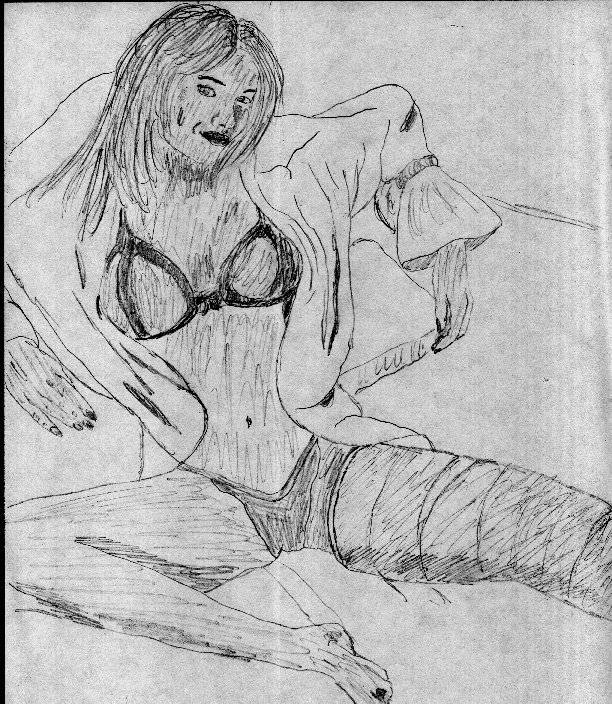
\includegraphics[width=\textwidth]{images/kicks03.jpg}
\end{center}

\chapter{A Way Out}
    Monique closed her textbook and sighed. She simply could not concentrate on global economics
tonight.

``This is college, I'm supposed to be having fun, not stressing myself to death,'' she muttered
to the empty apartment.

Monique was working her way through college, and not having an easy time at it. She was spending
so much time at her waitress job that her grades were starting to slip. On top of that, tips had
been sparse lately, and what once had been barely enough to see her through was just not enough
lately.

``Maybe I should just enroll at school back home,'' she added.

Of course, to do that would be to admit failure. She had told all of her family and friends that
she would make it, despite their protests. Now, there just wasn't enough money for books,
tuition and living expenses.

Her mother couldn't help: she was barely getting by as well. Her father had been an artist of
moderate success, and had moved the family to the United States when Monique was ten years old.
Five years later, when he died, he left Monique's mother with very little, and that had
evaporated quickly. Her mother worked long hours at menial jobs to keep food on the table and a
roof over their heads. Monique remembered the confident way she had told her mother that she was
going to go to college, and pay for it, herself.

As she was scolding herself for her pride and overconfidence, the front door swung open, and in
walked her roommate.

``Hey, Monique- what's going on?''

``Hello, Diane.''

Diane noticed the despair in Monique's voice

``What's wrong?''

``I can't concentrate worth a damn. Midterm is next week, and if I don't do well, I'm really
going to be in a hole with this class. Not that it's going to mean much in the long run, I'm not
even sure if I'm going to be able to come up with my part of the rent this month.''

``Come with me,'' Diane said. ``You're obviously in dire need of a beer or two. Besides, I have
an idea that just might ease your money crunch.''

``What would that be? A winning lottery ticket, or a rich, single doctor?''

``Neither. Just a job. Probably the strangest job you could ever have, but probably the easiest
and best paying one, too.''

``Now, I'm really wondering what sort of insanity you have in mind. What is it?''

``I'll tell you over a drink- my treat,'' Diane said.

At the pub, they each ordered a beer and sat at a corner table. Diane took a folded piece of
newspaper from her purse, opened it, then handed it to Monique. Monique looked at the classified
ad that had been circled. The heading was ``Models wanted, no experience necessary.''

After she had read the ad, Monique looked up to see that Diane had laid four one hundred dollar
bills side by side on the table in front of herself.

``You're looking at five hours work there,'' Diane said. ``Most of which was spent sitting on my
butt.''

``OK, what's the catch?''

``This guy is an artist. He does photography and sketches of women wearing casts.''

``WHAT?!?!?''

``That's right, casts. Just like one you would wear if you had broken a bone.''

``Before I ask why, can I ask why you? You're not wearing a cast.''

``No, I'm not,'' Diane replied ``But I was last week. He put a cast on my leg, took his
pictures, made his sketch,then took the cast off. He paid me, thanked me, and asked if I knew of
anyone else that might be interested in posing for him.''

Monique was truly puzzled, now.

``Why does he do this? Is it for some book or magazine?''

``That's the strangest part of it. He says that he does this for a rich patron. Supposedly, this
rich guy set him up with a studio, and foots the bill for all of this. I think the guy must get
off on it.''

``Alright, Di. You're kidding me, aren't you?''

``Monique, I swear this is true. As pinched as you are for cash right now, I'd never joke about
money.''

Monique finished her beer, then said: ``This is more than a little bit creepy, a rich guy who
gets turned on by women in casts?''

``It shocked the hell out of me, too. I almost got up and left when Quinn told me what he
wanted. The only reason I didn't was because he seemed like such a nice guy.''

``Quinn? Who is that? The rich freak?''

Diane asked the waitress for another round, then continued:

``No, Quinn is the artist. I never met the man who finances this.''

In her mind, Monique started to ponder this opportunity. It certainly was high on the
weird-o-meter, but four hundred dollars would give her some much needed breathing room in her
finances.

``So, what was this so-called artist like? You said his name was Quinn.''

``He was very nice. When he was putting the cast on my leg, he made sure that he didn't touch me
in any sexual way. I could tell he was being careful. And considering how high on my leg the
cast went, it wasn't easy. He might be gay, but it would be a shame-he's cute!''

``What about the cast? How did he make it? How did he take it off?''

``He did it just like a doctor would. Have you ever had a cast?''

``No''

``I had one when I broke my leg, and I remember how the doctor did my cast.'' Diane went on to
explain to Monique how the cast was made, and how it was removed. She made sure to tell her
about the removal saw, and how it would not cut skin.

``Alright, Diane--as broke as I am, I'll think about this. Do you think he would want to work
with me?''

``Monique- you are gorgeous. Between the way you look, and that little accent of yours, he's
bound to be charmed.''

``Alright, alright- I'll give him a call tomorrow.''

Diane handed Monique her cell phone.

``Call him now, while you still have your 'beer bravado.'''

Monique took the phone, and dialed the number in the ad.

\chapter{Angie}
After just under four weeks of running my ad in Kicks, I certainly have to call it a
success. I have had more calls than I thought I would get. Thus far, I've had the two casting
sessions with local women, both of which seem to have gone very well. I have another one
scheduled for today, and I even have had a referral! I will be interviewing a woman tomorrow who
was referred to me by Diane. Although I don't hold out much hope for this one, as she is a bit
standoffish, it is still remarkable to be recommended by a model!

At any rate, my job at hand is to prepare for Angie. Angie is a stunning young woman who is
going to look fantastic in a cast. I'm going to place her in a fiberglass long arm cast, so I
set out the necessary supplies: Purple fiberglass in three and four inch widths, three inch
padding, and three inch stockinette.

Angie arrived just a few minutes before 3:00 p.m. I took her inside and showed her to the cast
room. She removed her t-shirt and denim shorts, revealing the white camisole and underwear she
had told me she would wear.

``How's this?'' she asked.

She looked fantastic. ``That looks great. Would you like something to drink before we get
started?''

``No, I'm fine. I'm ready whenever you are.''

``Alright, first things first.'' I went into my usual routine of showing her the money, then
placing it with an envelope, and leaving it with her clothes.

``Thanks,'' she said. ``That is going to come in very handy.''

``Actually, I thank you, Angie. I'm always in need of more models for my work. Some people
change their minds about being a model when they hear that I want them to wear a cast. Some
people just find it to be too strange, though it's really harmless. The man I do this for would
never want to see anyone actually injured, he simply likes the way a beautiful woman looks in a
cast.''

``Oh, it's definitely strange, but as you said, nobody is getting hurt, so I don't see anything
wrong with it.''

``Exactly. If you're ready, let's get started.''

``Okay.''

I took the stockinette and cut off a piece a bit longer than Angie's arm. I slid the stockinette
up her arm, letting it bunch up at her armpit and overhang the fingertips slightly. I cut a
small ``V'' in the area over her thumb, then helped her get her thumb through the cut.

I took a roll of padding, and began wrapping at her wrist. After a turn to anchor it, I worked
it past her thumb, and made two turns to pad her hand. It covered her fingers too much, but I
would be trimming it back later. I instructed Angie to hold her wrist straight, with the palm of
her hand turned upward, and her elbow at a ninety degree bend. I continued up her arm,
overlapping each turn by half. This gave an almost completely uniform two layers of padding. The
first roll was not quite enough to get as high as I wanted the cast, so I had to start a second
roll. When I got to her armpit, I tore off the remainder of the roll, and set it aside. I
anchored the end of the padding with a piece of tape, and went to fill my bucket with warm
water.

When I returned, I checked to make sure Angie was still OK, and if she needed anything before we
continued.

``No, I'm fine. I'm just watching you work.''

``In that case, I'll continue.''

I took a plastic dropcloth and wrapped it loosely around her body, taping the ends together over
her left shoulder.

``This will keep the fiberglass from getting on your clothing or skin,'' I said.

I tore open a roll of three inch purple fiberglass and dipped it in the warm water. After the
bubbles stopped I wrung it out, and began wrapping Angie's arm at the wrist. I worked it over
her wrist and hand in a figure eight fashion, folding it into a ``Z'' where it passed between
her thumb and forefinger. After her wrist and hand were encased in four layers of fiberglass, I
finished the roll by working up her forearm. I then took my scissors and cut the excess padding
away from her fingers, leaving just a half inch protruding. I then cut the stockinette, leaving
enough to be folded over and anchored. I trimmed the stockinette and padding around the thumb so
that it, too could be anchored with the second roll of three inch fiberglass. I finished off
this roll by, once again, working toward the elbow.

The first roll of four inch fiberglass started at mid forearm, and I worked it all the way up to
her upper arm. Another roll of four inch followed, and by this time, I had the cast to its
desired height, which was just below the armpit. I folded over the stockinette and padding at
the top of the cast, And anchored it with a final roll of four inch fiberglass that continued
downward.

I pulled off my gloves, and tossed them into the trash.

``There it is, all finished. It's probably feeling pretty warm by now.''

``Yes, it has been for a bit- ever since you started the second roll.''

``That's just the chemical reaction of the fiberglass hardening. It won't get any hotter than it
is right now.''

``How long until it is completely dry?''

``It takes about thirty minutes for it to completely set up, but we don't need to wait quite
that long. After another ten minutes, we'll be ready to get started with the photos and
sketching. Would you like something to drink in the meantime?''

``Sure. Do you have anything diet?''

``That's all I drink,'' I said with a smile. ``Hang on.''

I went to get us each a soda, when I returned, I noticed her carefully examining her cast.

``So, what do you think of my work?''

``It looks fine to me,'' she said. ``I don't think it looks any different than ones I've seen
that were real.''

``It's made the same way that medical professionals make them. Let's see how it is drying.''

I examined the cast. It was still warm on the exterior. I wiped away the excess surface moisture
with a cloth. The stickiness from the resin was gone everywhere except the very top.

``It's almost dry. Let's give it a few more minutes, and we'll move to the other room.''

After we had finished our drinks, I removed the dropcloth that I had placed over her. She sat
there, in her skimpy clothing and huge arm cast, and I must say- she was breathtaking!

I retrieved my camera, and took a few photos of her sitting on the casting table. We then moved
to the studio, where I had her take a seat on the couch. After I had snapped several more photos
of her, I set her in the pose I wanted to sketch. I drew her from the right side, sitting in a
relaxed position. I made the cast totally the foreground of the drawing.

After I had finished, I showed her the sketch.

``Wow, that's really good. It certainly looks like me.''

``Thank you very much. I take quite a bit of pride in this,'' I said. ``Are you ready to get out
of that thing?''

She had a bit of a strange look on her face as she answered.

``Yes, I am, but it would be sort of interesting to wear this to classes for a day or so.''

``If you did that, a lot of people would ask questions. Even worse, if you had it one day, then
it was gone, they'd REALLY ask!''

``Yes, I guess they would, wouldn't they? Let's go ahead and take it off.''

I led her back to the casting room, and retrieved my Stryker saw and bandage scissors. After ten
minutes, her arm was free once again, and she put her clothes back on. As she slipped the money
into her pocket, she thanked me.

``No, Angie, it is I who thank you. You've been great to work with, and if you'd like, we can
certainly do this again.''

``I think I might like to. How about if I give you a call about it?''

``That's fine. If you decide against it, that's fine, as well. I've enjoyed working with you.''

``Thank you, it was nice working with you, too. I'd better be going, now. Goodbye.''

``Goodbye.''

After she left, I took the cut off cast, and took it to the basement and placed it with the
others. I returned to the casting room to clean up.

\chapter{Unexpected Inspiration}

\chapter{April}
Tuesday was a busy day. This evening will be my most adventurous casting session, yet. I
made sure that the camera was loaded and ready, then went to setting my supplies out on my cart.
Of course, I laid out a bit more than what I actually calculated that I would need, but it's
always better to have too much, than to be running to the closet while a cast is drying on a
model. When I finished, the cart was piled high, and I was ready.

April had looked very beautiful the night I interviewed her. She had been wearing a sweatshirt,
and jeans, and I could tell that she had a figure that begged to be casted. When she arrived
Tuesday evening, in shorts and a midriff top, I saw that my initial impression had been an
understatement. She could certainly have been a professional model, and in a much more
mainstream manner than what we were to be doing that evening. I led her inside, and had her sit
in the parlor, while I retrieved the envelope with the cash.

``April, I certainly appreciate your willingness to change the plans on such short notice.
Saturday night, my patron saw something that caught his interest, and he wanted me to do
something more along those lines.''

``That's not really a problem. It's a bit scary, not being able to move around much, but the
extra money will sure be nice.'' She replied.

``Speaking of the money, here it is. I always make sure that payment precedes performance,'' I
said, handing her the envelope.

She opened the envelope, discretely counted the money, then folded the envelope in half and
placed in the small overnight bag she had brought.

``I need a few minutes to change, where can I do that?'' She asked.

``Right through that door there,'' I said. ``I have one last-minute thing to do, and I'll be
ready. I'll be back in just a few minutes,'' was my answer.

She disappeared into the casting room, and I went to the kitchen to fill my casting bucket with
water.

I returned to the casting room, and tapped on the door before I entered.

``Come on in, I'm ready.''

When I entered, she had changed into what she had promised: a black, string bikini, which made
her look even more beautiful.

I placed the bucket of water with my cart, and led her to the casting table. I had her stand
next to the table, and pushed my cart to her side. I had her raise her arms, and I slipped a
length of eight-inch stockinette over her arms and body. I pulled it down to her knees.

I then made a downward cut about four inches long in the top of the stockinette under each arm.
Next, I took two cut broom handles, which I had readied earlier. I told her that she could use
them to support her arms, while she held them out to the side for me. After she had done this, I
pulled the stockinette up so the bottoms of the cuts were against her armpits. I then lapped the
flaps over her shoulders, and taped them down. I finished the stockinette by wrapping a section
of four-inch stockinette over her torso in a figure-eight style so that the stockinette laid
down around her breasts. I wanted this cast to accentuate her wonderful curves, not lessen them.

With this done, it was time for padding. I had to be careful, as this cast could easily become
uncomfortable if it were not padded correctly. After asking April if she was okay, took a roll
of six-inch padding, and began at her hips, working my way up. I made the padding three layers
thick, with an extra layer over her hipbones, for comfort. I began a second six-inch roll of
padding, and when I had wrapped up her torso, to her armpits, I tore off the remainder. I then
took a roll of four-inch padding, and worked it in the same figure eight manner as the
stockinette, covering her shoulders, and molding the padding to her figure.

``We're ready for the fiberglass, now. How are you doing?'' I asked her as I slipped on my
gloves.

``It feels fine so far. Like wearing tight clothes.''

``Well, it's about to feel very strange. You'll feel some pressure as I wrap the fiberglass
tape. Not heavy pressure- in fact, it will almost feel distant through the padding. As the
fiberglass starts to set, you'll feel heat, but nothing unbearable. The padding will insulate
you from it.''

``I'm ready.''

I tore open the foil wrapper on the first roll of five inch purple fiberglass. I wrapped it in
the same manner as the padding, starting too low on the hips, but I planned to trim the cast
after it had dried. I wrapped four rolls of five-inch fiber on her stomach and lower back, but
stopped just below the breasts. I then started with four inch purple fiberglass, and returned to
my figure-eight pattern.

After her entire torso was covered with purple fiberglass, I took a break. I asked her if she
needed anything to drink. She asked for water, so I got some, took the broom handle she held
with her right hand, handed her the glass of water and told her to be careful not to touch the
drying fiberglass with her arm.

``Why?''

``It is still setting. It is very hard to get off of skin, and it can irritate you pretty badly
.I don't want you itching, especially since it is going to be so hard to scratch.''

While she sipped her water, I picked up some of the mess that had accumulated so far, as there
was going to be more before we finished.

After the mess was picked up, I felt of her cast to see if it was set. It had become quite hard,
so I retrieved my cast saw.

``Let me trim this a bit, then we can finish it up, and you can sit down.''

I took the water glass from her, handed the broom handle back to her, and began to trim the cast
at her hips. I trimmed the cast so that it held her spine perfectly straight, but barely allowed
her to raise her legs perpendicular to her body. I then trimmed the cast a bit at the neck and
shoulders, smoothing out the edges, and making room to allow her arms to move fully. I then
pulled on a fresh pair of gloves, (the old ones were probably rock hard by now) folded back the
stockinette, and anchored the padding around her hips, neck, and shoulders.

Finally, there she sat, a beautiful woman, cast in a body cast that was, being honest, nicely
made. For a first attempt at a body cast, I was pleasantly surprised at how well it had turned
out.

``April, we need to let that cast set up for a little while longer before we go on. Does it feel
comfortable to you.''

``Yes, it's not uncomfortable at all. It feels like it isn't as warm inside as it was.''

``Good, that means it's almost set. In a few minutes, I'll let you get up and move around a bit
if you like.''

``I'd like to try using the rest room, if you think I can.''

``That might be tricky, but you should be alright.'' I was a bit worried about this- how would
she do at getting down, and then back up? I could, of course, help her, but that would be
uncomfortable to her, no doubt. I thought about it a few moments until an idea came to me. I
went and retrieved the aluminum crutches from the closet.

``Here. When you go, take these with you. You won't need them to walk, but you might need them
getting up and down in the bathroom. I'll stick close by the door, so if you need my help, just
call out. But if you don't, you can still have your privacy.''

``Thank you very much,'' she replied.

The bathroom trip went without incident. I helped her with the first few steps until she had
adjusted to walking without being able to flex her spine. I followed her to the rest room, and
waited while she was inside. I heard her shuffling to get down, and then I heard more shuffling
as she got back up, but she did it on her own, and thankfully didn't need my help.

As she emerged, she handed me the crutches. I noticed that her bikini bottom was now on the
outside of the cast. It seemed to make the whole thing look more realistic to me

``I'm ready to finish, now.'' She said.

I led her back to the casting room, and helped her sit on the table. I slipped three-inch
stockinette on her left arm all the way up to her shoulder, then cut it off just past her
fingertips. After making a slit and pulling her thumb through it, I wrapped her hand, wrist and
most of her forearm with two inch padding, and finished by using most of a roll of three inch
padding to wrap the arm all the way to her armpit.

I instructed April to hold her arm out away from the body cast, with the elbow slightly bent.
Most long arm casts have a ninety-degree bend at the elbow, but I have seen a few that were
almost straight, and I always liked the look. I suppose I like it because the arm is not nearly
as useful when it is casted in this manner.

I took one of the rolls of three inch purple fiberglass, and asked April if she were ready to
continue.

``Yes, I'm fine. In fact, it's really interesting, watching you work. It's also very weird to
experience it from the inside. It's like, one minute, I'm flexible and fine, but next thing I
know, I'm stuck.''

``So you're not getting claustrophobic or anything like that?'' I asked her.

``No, I'm really fine with this.''

I smiled and returned to my work. I dipped the first roll of three-inch fiberglass and started
wrapping it at her armpit. I worked down her arm until the roll ran out near her wrist. I folded
over the padding at the top of the cast, and anchored it with a second roll of fiberglass.

I then began using two inch purple fiber to wrap her forearm, wrist and hand, folding the roll
in the ``Z'' pattern between the forefinger and thumb. One roll built strength and thickness,
then I folded over the end and anchored it with a second roll.

``That arm is done,'' I announced. ``Ready for the other one?''

``Yes,'' she said, holding out her right arm.

I slipped more of the three-inch stockinette on her right arm, this time going only past the
elbow. I cut the thumbhole, and then wrapped her hand, wrist and forearm with a roll of two-inch
padding. One roll of three-inch fiberglass made an excellent base for the cast, and a second
roll anchored the padding and stockinette.

I stepped back and admired my work thus far. On my casting table was a beautiful blonde in a
long arm cast, a short arm cast, and a body jacket cast, All in purple fiberglass. Not exactly
what I had seen on the woman at the car show, but definitely inspired by her. One more thing to
do, and it will be perfect.

``April, we're down to one last cast to make.''

She scratched her nose with her freshly casted right hand, and smiled.

``I'm ready whenever you are. Which leg do you want?''

``Left,'' I said, moving the footstool over to where she sat.

She held out her left leg, and I slipped four-inch stockinette up to the top of her thigh. I
made sure to bunch it at the top slightly, as I planned for this cast to go up very high on the
leg. I grabbed a roll of 4 inch padding, and worked my way down from the top, so as to smooth
out the bunches in the padding with the next layer. Two and a half rolls of padding later, I had
fully covered her leg with 2 layers of padding, with a third layer at the ankle and knee.

``Are you still comfortable? No problems with going on?'' I asked.

``I'm fine. It's really kind of interesting, trying to move in these things. I'm sort of trying
to move my wrists, and my arm, and there's very little movement inside these casts. It's also
sort of wild, feeling the weight of the casts on me.''

``Well, then- lets finish this up.'' I said, pulling on another pair of gloves.

I took a roll of five inch purple fiberglass, dipped it, and began to wrap at the top of her
leg. I overlapped each turn of fiber by one half over the one before. I laid a second roll
directly over the first, making four layers on her thigh and knee. I folded over the padding and
stockinette at the top, and used a third roll to anchor it and give thickness to the top of the
cast. I then switched to four-inch fiberglass, and started just above the knee, working my way
down. Another roll directly over it, and I was done except for her foot. I took another roll of
four-inch fiber, and started at the ankle, working down to her toes, then back up to the rest of
the cast. I then folded over the padding, and anchored it with a fourth roll of four-inch
fiberglass. I added one more roll to the foot, ankle and lower leg areas to make certain that
the cast was good and strong, and my greatest work to date was complete!

``April, we're done casting. How does it all feel?''

``It feels okay, really.'' She answered. ``I sure wouldn't want to be like this for very long,
though.'' She added.

``It won't be long before we get you out. We can go do the sketch in a short while. Would you
like something to drink?''

``Yes, I'm getting thirsty.''

I went to the kitchen, and got sodas for each of us. I left mine in the can, but I poured hers
into a mug, so she could easily hold it with a casted hand. I also put a straw in it, so she
could drink without leaning back. As I returned with the drinks, she began to ask me questions.

``So, how did you come to do this? I mean, you don't see many ads in the paper for artists to
put casts on women, then draw pictures of them.''

``No, you don't,'' I replied. ``Let's just say I was in the right place at the right time.''

April wasn't letting go of the questions, though.

``So you get paid well for this?''

``Yes, I am well taken care of.''

``And this is what you want to keep doing with your life?''

She was really grilling me. It wasn't in any sort of flirtatious way, she was just being
curious. I finally ducked out of her questions by announcing that we were ready to move to the
other room.

I helped April to stand up and turn to her side. I then helped her to sit down in the
wheelchair. I placed the footrest under her casted left leg, and wheeled her into the parlor. I
retrieved my camera, and started taking pictures of her sitting in the wheelchair. I then helped
her from the chair to the sofa, and took some more photos.

Finally, I moved a table over to the French doors, and helped her to stand up and lean against
the table. Bathed in the sunlight, it was a beautiful place to sketch her. I asked if she
thought she could stand that way for a short time. She said that she could, and ran her casted
right hand through her hair. That was it. Perfect. I asked her to put her hand back to her head,
and I began to draw.

I worked quickly, as I was worried about her losing her balance and falling. The drawing took
shape very well, capturing her beauty, as well as her helplessness in the casts. After the
sketch was done, I helped her back to the wheelchair, and took her back to the casting room.

Once back in the casting room, I retrieved my removal equipment: cast saw, bandage scissors, and
cast spreaders.

``Which cast do you want out of first?''

``The body cast, please. It's starting to hurt my hips a little bit.''

``Absolutely. I see you looking at the saw sort of strangely. Let me show you how safe it is.''

I turned the saw on, and held the oscillating blade to my bare hand. I then showed her that the
cast did not cut my skin.

``This saw only cuts hard objects. Anything soft, it just vibrates on.'' I could see the relief
in her eyes, so I instructed her to lie down, and helped her to do so.

I quickly cut through each ``strap'' over her shoulders, then raised her arms above her head,
and cut each side from armpit to hip. I pried the cast apart a bit with the spreaders, and then
cut through the padding and stockinette down one side with the bandage scissors, making sure not
to cut the straps of her bikini top.

I then placed her arms back at her sides, and cut through the padding and stockinette over each
shoulder. I then opened the cast, almost like a book, and helped her to sit up, freed from the
fiberglass. I noticed that the stockinette had imprinted its pattern on her skin.

I quickly cut each of arm casts in a similar fashion: cutting through the cast on both sides,
but only through the soft material underneath on one side, allowing the casts to open like a
book. I removed the leg cast by cutting down the side, going under her heel, then back up the
opposite side with one long cut. Once the padding and stockinette was cut on one side, I was
able to open the cast, and removed her leg and foot from the back, leaving the entire foot area
of the cast intact.

Once free, April put her clothes and shoes back on. Before she left, we thanked each other, and
I left her with an open invitation to call if she ever wanted to work with me again. She said
that she might, and left.

Once she was gone, I gathered the cutoff casts, and placed them in the basement with then
others. My collection was growing. As I returned upstairs to clean up the casting room, I
wondered if I was becoming addicted to this. Was it going to take more and more to satisfy me?
Is it going to take more and bigger casts? If it is, is it such a bad thing?

\begin{center}
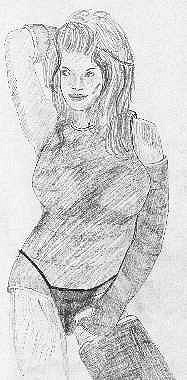
\includegraphics{images/kicks07.jpg}
\end{center}

\chapter{Monique}
``What are you getting yourself into?'' Monique wondered to herself as she knocked on the
door of the old house.

``Staying in school and refusing to fail at what I've started-that's what'' she reminded
herself as she waited. After all, what would be so bad about it? Diane had told her that this
``artist'' had been very respectful and honorable to her.

It's just so bizarre, though. Stripping to her underwear, then letting a total stranger put
a cast on her, then allowing him to take photos and make a drawing of her. What sort of person
WAS this artist, anyway?

``The sort of person who is going to help me get the bills paid this month,'' she said to
herself as the door opened.

The man who answered the door was not at all the short, bald, middle aged man she had
pictured him as. He was in his mid to late twenties, rather attractive, (or so Monique thought)
with very deep and expressive brown eyes that looked straight into hers. In fact, the only thing
about him that she had expected was his goatee.

He caught her a bit off-guard by looking her in the eye. Monique was used to men taking
stock of her attributes from the neck down before even bothering to notice if she even HAD eyes.

``I'm Monique, are you Quinn?'' She asked, hoping that this was indeed the man she was here
to see.

``Yes, please come in,'' He said opening the door for her.

``My God, this woman is beyond beautiful,'' I thought to myself as I looked at Monique. She
had long brown hair, beautifully formed facial features, and her eyes-piercing and strong, yet
revealing a softness and vulnerability that I assumed she showed to very few, if any, people.

``Please, have a seat. Would you like anything to drink?''

``Water is fine,'' she said. ``Mind if I smoke?''

``Not at all, there's an ashtray on the end table.''

In the kitchen, I dropped ice into the glasses, then filled hers with water, and mine with a
diet soda. ``Get a hold on yourself, Quinn,'' I thought. ``Be professional- she is just your
model, this is not some sort of date. She would not be here if it were not for the money. Don't
let yourself forget that, or you could wind up in serious trouble.''

After composing myself, I returned to the living room, handed her drink to her, and sat down
across from her. I tried to make some small talk, but her answer to every question was short,
almost on the edge of being impolite.

She definitely had some walls around her, this one. I didn't press the issue of getting more
comfortable with each other, as I did not want to seem inappropriate. In the end, this was
nothing more than a business arrangement, so business is what I got down to.

``So, have you ever worn a cast before?''

``No.''

``But Diane told you what it was like, I assume.''

``She said it was safe and painless, she said you were professional, and she said you pay
well.''

``Alright, do you have any questions about this whole thing?''

``Yes- when do we start, and when do I get paid?''

I couldn't help but smile. ``We start just after you get paid, and you get paid as soon as
we get into the application room.''

``I'm ready when you are.'' was her reply

I led her to the application room, and told her I would leave her alone to get ready. As I
went to retrieve the bucket, and fill it with warm water, my mind was certainly not thinking
totally straight. This woman was beautiful, exceptionally so. I've seen more than a few
beautiful women, but this one was even more beautiful than most. Her attitude, on the other
hand, was a shame. To have such exquisite beauty, with such a standoffish demeanor seemed almost
like a cruel joke. Oh well, it was only business anyway.

\begin{thought}
``Nice going- you were really a total bitch.'' Monique thought to herself as she slipped out
of her jeans. ``This guy seems nice enough. Why did you have to be so mean?'' ``Because it's a
mean world, and you have to be strong to survive, that's why,'' she muttered to herself.
Besides, what this guy is doing, no matter how nice he is, no matter how cute he is, is simply
NOT normal.'' ``Oh well, he's just making a living, trying to survive like the rest of us,'' She
thought as he came back to the room.
\end{thought}

When I returned to Monique, I almost let myself stare too long at her. In her lacy, pale
blue bra and matching underwear, she was breathtaking. In addition to the striking beauty of her
face, she had the figure to match: long, graceful, well proportioned curves, and a fabulous tan.

``As promised, payment before we start,'' I said, taking the envelope from the casting
table. She took the money from the envelope, counted it, put it back in the envelope, and then
placed it with her clothes that were neatly folded on the table by the door. As she counted the
money, I couldn't help but notice a flicker of what might have been relief in her eyes. That
expression faded as quickly as it came. She held her hands out to her side and asked ``Are you
ready?''

``Absolutely.'' I motioned to the table. ``Have a seat.''

She hopped up on the table, and asked ``So, where do we start?''

``Let's do the arm first,'' I said talking her left arm in my hands. ``Hold it out straight
for me.''

I pushed my cart to her side, and reached for the three-inch stockinette. I unrolled it, and
slid it up her arm to the armpit. I then cut it off at the end of her fingers.

``OK, now I need for you to hold your elbow at a ninety degree angle, with your thumb facing
upward.'' After she did this, I made a small slit in the stockinette over her thumb, and pulled
her thumb through. I then took a small length of one-inch stockinette, and placed it over her
thumb, positioning it straight upwards.

``Now, just hold that pose while I apply the padding.''

I wrapped two even layers of padding over her whole arm, wrist and thumb. I used two-inch
padding for the thumb and hand, and three-inch for the rest of the arm. I taped the tail of the
last roll down where it ended at her armpit. She was ready for the plaster.

I took a roll of the two-inch plaster from the cart, dipped it, and started at her wrist. I
worked the roll over her wrist, hand, and thumb. I repeated this with a second roll, then I
quickly took my scissors and trimmed the padding and stockinette back, folded it over, then
anchored everything with a third roll of two-inch plaster. I then dipped a roll of three-inch
plaster, and began where the previous plaster had stopped, working it from her wrist to just
past her elbow. Another roll followed pretty much over this same area. The next roll was used
entirely over the elbow, back and forth, to give the elbow strength. The next two rolls extended
the cast to within two inches of her armpit, and the final roll anchored the stockinette and
padding at the top, and gave some added thickness to the rest of the cast. I finished the cast
by smoothing out the plaster with my hands. I looked up at Monique.

``Is it getting warm, yet?''

``Yes, it's very warm around my thumb and hand.''

``It's not unbearable, is it?'' I asked.

``No, but it's very heavy,'' she replied.

I tapped the setting plaster with my hand, and realized that it was ready for the final
smoothing.

``Hold tight, it's not quite hard enough to rest it on anything, yet. I have a bit more
smoothing to do in the meantime.''

I took a sponge, dipped it in the water, and rubbed it over the rapidly setting plaster,
giving it a very smooth surface. This cast was turning out very nicely. After this was done, I
held the cast so that the weight on her shoulder would not be uncomfortable. I held the cast
with the palms of my hands, so as not to dent the cast and make a pressure spot. Although my
casts never live for more than a few hours, I still try to make them perfect, and above all,
comfortable.

``Is that better- with the weight?'' I asked.

``Yes, it helps,'' she said curtly.

As the plaster got warmer under my hands, I tapped the surface, and decided it was probably
safe to rest it on something. I asked her to hold it for a moment, and I retrieved a
plastic-covered pillow and a box that seemed about the right height. I placed the box beside
her, put the pillow on top of the box, and gently laid her arm on it.

``There, is that comfortable?''

``Yes.''

I rinsed my hands in the bucket, then dried them off with a towel. ``Let's take a break
before we do your leg.'' I took out my cigarettes and offered her one. ``Smoke?''

``Yes,'' she said, ``but I want one of mine. They're over with my clothes.''

I got her one of her own cigarettes, gave it to her, then lit it. (At least she let me do
THAT) I then lit one of my own for myself.

\begin{thought}
``This really doesn't feel bad at all,'' Monique thought to herself as Quinn was putting her
arm in a cast. She noticed how his hands were firm, yet gentle as he wrapped the plaster on her
arm. She found herself intently watching what he was doing. At first, she watched with
curiosity, simply wanting to see how the cast was made. Soon, however, she became fascinated by
his hands- the way she could feel them working the plaster, but how that feeling was diminishing
with each passing moment as the plaster began to set. She snapped out of her fascination when he
asked if it was getting warmer. She quickly put the enjoyment of watching him work behind her
before she answered him. She HAD to keep her distance. Still, she did have to admit to herself
that the cast looked very professional. She'd never seen a cast that went all the way to the
armpit, and covered the thumb as well. Quinn had told her over the phone that casts such as this
were actually used for certain types of injuries. The cast felt like nothing she had ever
experienced before. It was heavy, and it certainly looked hard on the outside, but it was soft
and comfortable on the inside. She tried moving her thumb inside the cast, but it would not
budge- it was held fast. She wanted to touch the outside of the cast with her other hand, but
she decided not to, since Quinn was being so careful as he touched it. If he was being careful,
maybe touching it might damage it in some way.
\end{thought}

``Well, Monique, now you can no longer say that you've never worn a cast. What do you think
of it?''

Monique quickly went back into her defensive mode. ``Well, it would suck to have to wear one
for two or three months, that's for sure. I guess it's not so bad this way, especially since I'm
being paid to wear it.''

``Damn, is money all she thinks about?'' I asked myself at her remark. I've seen this type
of woman all my life- all they care about is money, and what it buys them. What a waste- she is
so beautiful, and has no substance to back it up with. I noticed an increasing dislike for her
building inside me. ``Oh well, at least she is easy to look at. I'll try to get this next cast
done quickly, and be done with her,'' I thought to myself.

``Yes, the money does make it easier, doesn't it?'' I replied, trying to remain civil. ``The
boss does pay well.''

``Does this boss, or patron, or whatever you call him have a name?'' She asked.

``Yes, he does, but he is a public figure. He feels that if anyone ever found out about
this, it could lead to undesirable consequences for him.'' That was as much of an answer as she
needed- Hell, for all I know, she might have wanted to know so she could go find this
non-existent person, and throw herself at him- and his money, of course. With her looks, she'd
probably end up marrying money. I've seen way too many women like this in my time- they disgust
me. I snapped myself out of my contempt enough to go on.

``Well, are you ready to do your leg?'' I asked.

``Yes, if you are.''

``Then let's get started.''

I took her left leg, and rested it in the stand I had made for casting legs. The stand
rested on the floor, and had a bar going straight upwards. (Actually, it was nothing more than a
rolling stool with the seat removed) I had welded a U-shaped stirrup to the top of it, so that a
leg could rest in it. For comfort to uncasted legs, and to prevent damage to fresh casts, I had
padded the stirrup heavily. The height was adjustable, and I was very pleased with this
invention.

With her leg in the stand, I took my four-inch stockinette, and unrolled it until I was sure
there was enough to cover her leg. I held it up to her leg, and mentally figured how much extra
I would need, (stockinette tubes get shorter as they stretch in diameter) and cut it off. As I
slid the stockinette over her leg, I noticed a small scar on her knee. I guess those ``perfect''
legs aren't so perfect after all. As I slid the stockinette up to the top of her thigh, and
bunched a bit of it there, I noticed that she was watching me closely. Probably so she could
raise hell if I touched her in any inappropriate way. I was, of course, very careful not to.

I quickly worked the padding onto her leg. I used four-inch around her foot and ankle and
six-inch over the rest of it. I made sure to use my normal overlapping style of wrapping so that
she had an even two layers over the entire cast, with an extra layer at the knee and ankle. Her
leg was now ready for the plaster.

``Is your arm still alright?'' I asked her, wanting to make sure that the previous work
wasn't giving her any trouble.

``It's fine,'' she said ``The heat isn't as bad as it was.''

``Good. That means that it is pretty well set.'' I told her.

``Is it dry? Can I touch it, or try to move it?'' She asked.

``No, plaster doesn't fully set for about 24 hours,'' I answered. ``You can touch it if you
like, and you can try moving it a little bit, but don't strain against it at all- it could still
break easily. Are you ready for more of the same on this leg?''

``Sure. Go ahead''

As she explored her arm cast from both inside and out, I took a roll of four-inch plaster,
dipped it, and began wrapping it around her ankle. At first, I used a figure-eight pattern, to
hold the ankle in place, then I wrapped the entire ankle for thickness and coverage. The second
and third rolls, one on top of the other, started at her foot, and worked over her ankle, to
just slightly on her calf. I trimmed the stockinette and padding, folded it over, and anchored
it with a fourth roll of four-inch plaster. I then began working with the six-inch plaster. I
began where the four-inch left off, working the roll to just past the knee. Three more rolls
mirrored this one, then the fifth roll of six-inch plaster started just blow the knee, and ended
at mid thigh, thereby strengthening the knee. Two more rolls of six inch gave a good thickness
for her thigh, and after I had trimmed and folded the stockinette and padding, one final roll
anchored it, and gave more thickness to the thigh. I smoothed out the plaster, and after the
sponge smoothing, it was set enough at the ankle to put back in the foot rest that I had made. I
looked at my work, and I have to say, it turned out very nicely.

``Well, we need to let that dry awhile before we move you.'' I told her. ``Let me get you
your cigarettes.'' I handed her the cigarettes and lighter (she can light it herself, this time)
and asked if she needed more to drink. She agreed to a soda, and so I went to get one for each
of us.

\begin{thought}
``Pull yourself together!'' Monique thought to herself after Quinn had left the room. Her
leg tingled with the heat of the setting plaster and she had to admit she found it pleasant. She
had really been amazed, watching him work. He had been very professional, never touching her in
any inappropriate way, even though he could have done so and made it seem totally accidental.
For a brief moment, she found herself wishing he had. In the next moment, she wondered if he
might be gay. ``It doesn't matter, stupid, this is money, nothing more. What happens when you
get close to someone? You get weak, that's what happens. And what happens when you get weak? You
lose control, and then you get HURT. Just let him take his pictures, do his drawing, or whatever
it is, then get the hell out of these casts, and go save your ass with the money!'' She thought
again about the casts. It sure would be difficult trying to get through daily life with these.
She pictured herself trying to get back home while still wearing them. She smiled as she thought
to herself. ``No, not even little miss ‘I don't need anyone' could do that. Then she thought
``Bullshit- I'd find a way- I always do, don't I?''
\end{thought}

I returned to the casting room to find Monique deep in thought. ``Are you in there?'' I
asked, breaking her ``trance.''

``Yes,'' she replied instantly. She took the soda from my hand ``Thank you.''

Over the next 20 minutes, I engaged her in some forced conversation about her schooling and
activities. It wasn't a pleasant conversation, by any means, but it avoided the uncomfortable
silence that was the alternative.

She was definitely guarded, that's for sure. She didn't give me very much personal
information. Not that I wanted it, I didn't feel any desire to get to know her any more than she
appeared to want to get to know me. Of course, I'm sure, had she seen my bank statements and
stock portfolios, she would have been much friendlier. To hell with that. Not to belabor the
point, but I've seen too many like her before.

After we had let the leg cast harden for a bit, I asked her if she was ready for me to take
her into the other room for the final part of the session. She said she was ready, so I told her
how we were going to move her: I told her that I would help her stand up, then we would turn
her, and I would help her sit down in the wheelchair. I pushed the wheelchair to the side of the
table, locked the wheels, and moved the leg rests out of the way. I took her uncasted right arm,
put my other arm behind her, and helped her to stand on her uncasted right leg. We then turned,
and we sat her down in the wheelchair, smoothly and gently. I held her casted leg up with one
hand, and positioned the leg rest under it with the other. I then moved the other leg rest into
position, and she placed her foot on it.

I wheeled her into the living room, where we placed her on the couch for several photos in
different positions. I then helped her back into the wheelchair, and moved her to the window,
where we took more photos. I decided to have her standing for the sketch, so I helped her stand
up, and lean against the antique table as I drew.

The drawing was rather uninspired, given my mental state where she was concerned. I didn't
feel like I had captured the essence of her facial features very well at all. Despite this, when
I showed it to her, she said that it looked very good. As she said it, I couldn't help but
notice what seemed to be sadness in her eyes.

``If you're ready, we can get you out of these, now,'' I said.

``Definitely,'' she replied.

``Oh, you didn't like them?''

``It's not that bad,'' she answered. ``Just the same, I'm ready to have my arm and leg
back.''

I helped her back into the wheelchair, and then back to the casting room. Once she was back
on the table, I gave her my usual talk about the cast saw, and how it would not cut skin,
complete with a demonstration of my holding the humming saw to my bare hand with no injury.

I made two quick cuts, one on each side, through the plaster of each cast. I made one pass
through each cast with the bandage scissors, and the casts opened up and she was free. I left
her to get dressed.

Once dressed, she came out of the casting room.

``Thank you,'' she said in a surprisingly polite tone, maybe even a bit sad. ``This cash
will come in very handy.''

``Thank you, Monique, you're a very beautiful model, and I enjoyed working with you.'' A bit
of a lie- I admit, I stopped enjoying working with her halfway through it, but I didn't want to
be rude.

``Do you ever do repeat sittings with a model?'' She asked ``This wasn't so bad, and I
wouldn't mind maybe doing it again.''

``Well, I'm not opposed to it.'' OK, a bigger lie that time, ``But since I'm not the one
financing this, we'll have to see what the money man thinks of our work. Why don't you give me a
call in a week or two?'' What was I saying? I wanted this gold-digger gone. The words had just
come out before I knew what I was saying.

``OK, I'll be in touch,'' she said as she left.

``Whatever.'' I muttered to myself after the door closed behind her. I went to clean up the
castroom.

\begin{thought}
``Why did you say that!? Why!? Why!? You IDIOT! Monique scolded herself as she walked back
to her apartment. She went most everywhere on foot these days, since her old Firebird was long
dead of terminal transmission failure.

``Why did you ask to do it again? Why did you show that little sign of weakness?'' She
answered herself with ``Because I need the money, that's why.'' And deep down inside her, her
inner voice told her a couple of other things. Things she didn't want to hear, things she
refused to admit.
\end{thought}

\begin{center}
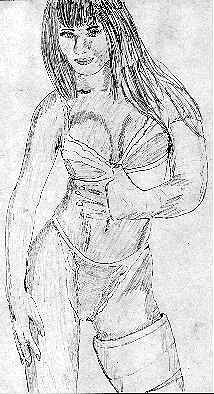
\includegraphics{images/kicks08.jpg}
\end{center}

\chapter{Tanya}
As Spring rolled into Summer, my phone didn't ring nearly as much. No doubt, this was caused
by the fact that most students went home for the summer, or were off doing other things, once
the spring semester finished.

With plenty of time on my hands, I decided to get away for awhile, so I got on a plane and
headed for the Bahamas. The trip was wonderful- sun and sand are always good for the soul.

While in Nassau, I had a very pleasant cast encounter. I was walking along the beach when I
saw her. She was tall and blonde, with very pleasant looking facial features. She wore her hair
pulled back into a pony tail, and covered with a baseball cap. She wore an oversized printed
white T-shirt, canvas shorts, and a flip-flop sandal on her left foot. Her left foot, however,
is not what you want to hear about, is it?

Her right leg was covered in blue fiberglass. It started at her toes and went all the way up
until it disappeared under the khaki colored shorts.

The fiberglass was a darker blue than any I'd seen before- it was actually a navy blue, and
I liked the color instantly.

She had a small gym bag in one hand, and carried aluminum crutches under the other as she
hobbled out nearer to the water. I noticed she had a plastic bag over the toes of her casted
foot, and that it was secured with a rubber band. Good idea- I can imagine that sand in a cast
would not be very comfortable!

I followed her with my eyes until she had gotten to a point on the beach that she liked. She
dropped the crutches, and opened the gym bag. She pulled a large beach towel from it, and spread
it out on the white sand. She then proceeded to unfasten her shorts and let them fall to the
ground. She quickly hopped her left foot out, then carefully, with as much grace as possible,
lowered herself to the ground. Once down, she leaned forward, and slipped the shorts off of her
casted foot. She then removed the T-shirt, revealing the black bikini she wore underneath.

It was obvious that sunbathing was a normal pastime for her, as she had a very beautiful,
natural looking tan. She finished preparing by removing the plastic bag from her right toes,
revealing that the toenails were painted to match the cast- cute touch.

I kicked myself for not having my camera with me- what a great candid photo this would have
made! I decided to go back to my room to get the camera. With all of the trouble she went
through to get to that beach, she probably was not going to leave anytime soon.

Back at my hotel room, I glanced at my cell phone to see if the indicator showed any voice
mail. It did, so I called to retrieve my message.

``Hello, my name is Tanya, and I'm calling in regard to your ad for models. Please call me
back,'' and she left her number. Since my sighting had me in ‘full casting mode,'' I decided to
call her back immediately.

``Hello,'' said the pleasant female voice.

``May I speak to Tanya?''

``This is Tanya,'' returned the pleasant voice.

``Hi, I'm returning your call about the modeling job.''

``I'm curious as to what sort of modeling it is.'' The on the spot question. I thought of the
casted woman on the beach. I didn't want to lose the photo opportunity, so I didn't hedge around
the subject.

``Tanya, for this job, you will be placed on one or more medical style casts. Afterwards, I
will take photos of you in your cast, then make a sketch of you.'' There, that was a quick
enough
way to say it. The phone line was silent for a few moments, followed by her saying ``What?''

``It's true,'' I said, launching into my canned cover story about the moneyed patron and my
assignment.

Another pause, then she said ``That's really bizarre. How much does it pay? How long does it
take?''

``It usually takes three to five hours, depending of the type and number of casts, and the
pay varies, as well. The more you are casted, the more money you are paid. The absolute minimum
is three hundred dollars.''

``That's not bad money for a half day's work. So, would I be nude except for the casts?''

``No, absolutely not,'' I replied. ``We like for you to wear either lingerie or a bathing suit
for the sessions.''

``Wow, that really is bizarre,'' she said ``but I could use the money. How soon could we do
it?''

``Tanya, I can't commit to doing it until I see you in person. The man paying for this likes
certain types of women, and I'd have to be sure you fit in.''

``I see. When can we meet?'' she asked. She must have been in need of quick cash.

``Let's do this- We'll meet Friday at 2:00 p.m. Bring along a bathing suit or lingerie. That
way, assuming you're the type we're looking for, we can go ahead and do it then, OK?''

``That sounds great. Where do I need to be?'' I gave her the address, and told her I was
looking forward to meeting her.

After I hung up, my casting excitement was at full stir. I began packing so I could get home
and get ready. I was halfway through my call to the airline when I remembered the woman in the
LLC on the beach.

``Shit!'' I said. I finished the reservation call, grabbed my camera, and rushed back out to
the beach- my subject, however was gone. I kicked myself for not having the camera with me in
the first place. Still, it was a very nice sighting, and I'd never seen fiberglass in that dark
of a blue before. I made a mental note to find some of that color as I headed back to the hotel.
The stranger on the beach, destined for some very odd tan lines, remained on my mind all the way
home.

Thursday was very busy- After gathering up the pile of newspapers, and dusting, I made a
trip to renew my supply of plaster. The long leg cast and long arm thumb spica that I had made
on Monique had dwindled my supply. Yuck, why did I have to go and think about HER? Lousy
gold-digger.

``Because,'' I answered myself aloud, ``gold digger or not, she looked fantastic in those
casts!'' Whatever. It was a shame that all that beauty was wasted on a woman with so little
substance.

After I returned from the supply run, I relaxed on the front porch with a Diet Coke and a
cigarette, while my mind played out different casting scenarios possible for Tanya.

Friday, at ten minutes past two, the doorbell rang. I opened the door to a woman of
remarkable beauty. She had long permed brown hair, brown eyes, and very pleasant facial
features. As I let my eyes drift down, I quickly realized that she definitely ``fit in'' as a
model.

``Tanya?''

``Yes. You must be Quinn. I'm sorry I'm late, but I got lost.'' She said with a smile.

``That's not a problem. Come in,'' I said, leading her to the parlor, and motioning for her to
sit. I offered her a soda, and by the time I had returned, I knew how I wanted to cast her, as
long as she was willing.

``Tanya,'' I said as I sat down, ``what I would like to do is to put you in a shoulder spica
cast.''

``I guess that means I qualify.'' She said with a sly smile.

``Definitely. You're more than qualified.'' I smiled back.

``So, what is this shoulder spica cast?''

``A shoulder spica cast starts at your waist, covers your torso, one shoulder, and that
entire arm as well. Medically, it is used to immobilize fractures of the upper arm bone. It is a
big, heavy cast, and I'll pay you \$450.00 for modeling it.''

``Wow. Very good money. How do you get me out of it once we're through?''

``The exact same way that a doctor would. Come with me and I'll show you.''

I led her into the casting room, and retrieved the cast saw from its place in the cabinet. I
plugged the saw in, turned it on, and held the oscillating blade against my left hand.

``This instrument is a medical cast saw. ``I began. ``the blade moves back and forth instead of
rotating. What this means is that it will cut hard objects very well, but with something soft,
like skin, it simply vibrates. It's totally safe- there's no way it can cut you.''

``Well,'' she said ``I've never worn a cast before, so I might as well start big. ``I'm ready
whenever you are.''

``Alright, I'll leave you to get ready. What did you bring to wear?''

``I brought a swimsuit along. It's a one-piece. I also, of course, have my underwear on
beneath my clothes.''

``Let's just go with the underwear,'' I said. ``Considering the type of cast we're going to be
making on you, a one piece swimsuit could cause major troubles if you need to use the
restroom.''

``Yes, I suppose that could be a very bad thing,'' she said with a slight smile.

I left her and quickly went to the garage. I got an old hacksaw and a broom handle that I
had kept around for this occasion. On my way back, I stopped in the kitchen for an envelope. I
placed the bills inside, and returned to the casting room. Tanya's eyes got huge when she saw
the hacksaw.

``This is just to cut the brace that helps hold your arm out,'' I reassured her.

Standing there, in nothing but her white underwear, she looked amazing. She was going to
make an excellent model for this cast! I asked her to slide her bra strap under her arm on the
right side, as that shoulder would remain bare. When she had done this, I handed her the
envelope and said: ``If you're ready, we'll begin.'' She looked in the envelope, nodded her
head,
and I began working.

I took my roll of twelve inch stockinette, and cut off four feet of it. I had her hold her
arms straight up while I slid it down over her body, past her hips. I then made slits down each
side from the top to where the stockinette rested under her armpits, and allowed her to lower
her arms. I pulled the front and back halves of the stockinette together over her left shoulder
and taped them into place. I then took a roll of three inch stockinette, and slid this onto her
left arm all the way to her shoulder. I trimmed this off at her fingertips, and made a slit for
her thumb to pass through. As I was doing this, I was explaining the process to her: ``This is
stockinette, which keeps the padding from irritating your skin. Next comes the padding, which
will make this cast much more comfortable to wear. What I need for you to do is to hold your arm
out at your side like this.'' I took her arm, and held it so that her upper arm was at a 90
degree angle to her body, and the elbow at a 90 degree angle. I then handed her the broom handle
to hold onto to steady her arm and keep her muscles from fatiguing.

I took a roll of 6 inch padding, and began wrapping her body at the hips. I worked my way up
over her waist and torso, keeping the padding slightly taut so that it would conform to her
curves without bunching. As I got to her chest, I loosened my wrapping just a bit, however. I
then took a roll of four inch padding, and began wrapping her upper arm, working over the
shoulder. I made a couple of passes between her breasts in a figure-eight style so that there
would be some separation. I took another roll of six inch padding, and used it to cover her
lower torso again, paying particular attention to her hip bones, since they bear a lot of the
weight of a shoulder spica. One more roll of four inch finished the upper torso and shoulder,
and two rolls of three inch took care of the rest of the arm and hand.

With her all padded and ready, I quickly measured the distance from her forearm to her hip
bone,, and took the broom handle from her just long enough to cut a piece to length. I gave it
back to her, and we were ready.

Nothing looks better for a shoulder spica than plaster, but I was afraid that it would take
forever to dry. I had decided to get a bit clever, though.

``Tanya, this type of cast looks much better in plaster. However, plaster takes a long time
to dry, and it would be very tiring on you having to wait. What I am going to do is to first
make the cast in fiberglass, then cover the fiberglass with a layer of plaster. In the end, it
will look every bit as good, but the process will be much easier for you this way.''

``If you say it's better this way, I appreciate your doing it like this.'' She replied.

I excused myself long enough to get the water. I filled the bucket with water at about room
temperature for the fiberglass. When I returned, I found her poking at the padding a bit with
her free hand.

``Checking it out?'' I asked.

``I was just seeing what it felt like on the outside,'' she replied. ``This is new to me, and
I'm just curious, that's all.''

``That's no problem. If you're ready, here's where it really gets interesting.'' I took out
several foil packets, and laid them on the table next to her.

``These are the fiberglass bandages. I will first dip them in the water, then start wrapping
them on you. As they begin to set, which will only be a few minutes, you will feel them getting
warm. The heat shouldn't be too uncomfortable, but if it gets that way, be sure to tell me.''

``OK''

I opened the first roll of four inch white fiberglass, dipped it, and began wrapping her
upper arm. I worked my way over her shoulder, and chest, being careful not to smash her breasts
under the bandage. I began where I did so that this area would begin to set up first. The next
roll was five inch, and I used it to continue the cast down to her hips. I then took another
roll of five inch, and laid it directly over the last one. I then took two more rolls of four
inch, and wrapped them over her chest, shoulder and upper arm, to strengthen this area. Once
this was done, I used three more rolls of four inch to cover her arm down to the wrist, and a
roll of three inch for her hand. I finished the fiberglass work with one final roll of five inch
from her hips to her chest. I could see the water sweating out of the fiberglass in places, and
I felt the heat from the exothermic reaction of the fiber.

``We're all done with that part, Tanya- how is the heat?''

``It's not bad. I can feel it, but it's not uncomfortable, though.''

``Good. In a few minutes, you won't need the broom handle anymore. That fiberglass gets solid
fast.''

``It's almost kind of $\ldots$ Cozy,'' she said.'' Can I relax my arm, yet- It's starting to get
tired.''

``Not just yet, but soon- it's got to sound good by now, though.''

``Actually,'' she confessed ''I'm mostly relaxed already. I hope that doesn't screw things
up.''

``For what we're doing, probably not. Just don't try to strain against it.''

``OK''

I excused myself again to change the water in the bucket. This time I got water as hot as I
could stand. With an entire cast already on, the heat wouldn't bother her, and it would make the
plaster set quicker. When I returned, I asked if she was ready to continue. She nodded.

I began by trimming the padding back to the edges of the cast, and then trimmed the
stockinette, leaving it long enough to anchor. Now, for the plaster!

I began with a roll of five inch plaster, and began at her hips. I worked upwards, using two
layers of plaster over the fiberglass. I found two layers to be enough to make the cast look
like it were constructed solely out of plaster. Five more rolls of plaster in varying widths
covered the fiberglass very nicely. When that was done, I took another roll of four inch, held
the broom handle in place, and carefully plastered it to her waist. This was tricky, and another
pair of hands would have been nice, but I managed. One more roll of three inch plaster anchored
the broom handle to her forearm, and covered the wood. I'm sure that it wasn't as strong as it
would need to be for a full plaster shoulder spica, but, like the plaster, the bar was only for
show anyway.

It only took about ten minutes for the plaster to get pretty well set. It was still damp,
and giving off a lot of heat, but it was Ok for her to move around, by this point, the
fiberglass was pretty well as hard as it was going to get. I asked if she needed anything before
we moved on the photos and sketching. She said she could use a trip to the restroom, so I led
her there, told her to be careful, and waited outside in case she needed any help. As she came
out, she said: ``Wow, this thing weighs a ton!''

``Is it comfortable,'' I asked. ``can you breathe easily?''

``It's not uncomfortable. It's odd, but it's kind of cozy. It's very strange not being able
to move my arm at all. It almost seems as though it's not even a part of me. It just moves with
my body.''

``Actually, that's a fairly common reaction from someone wearing their first cast,'' I
replied. ``Are you ready to finish?''

``Yes.''

I led her to the back bedroom, and had her sit in the chair by the window. The outside made
a nice backdrop- it gave a sense of connection with the outside world. I remember thinking to
myself how fantastic it would be to take a beautiful woman outside, casted like this. Not only
outside, but out in public- it would be great to watch the reactions of the people we
encountered. Of course, it was impossible- this was a small college town. Even if a model were
that brave, she would either have to wear the cast for a full term, or explain why she had the
cast for only one day. I'd rather not have too many people know what I was doing, as I'm sure
there would be a negative backlash.

I took several photos of her, then I decided to have her stand by the bed for the sketch.
This would be a very sensual pose. She stood next to the bed, and even placed one knee on it, so
she was halfway on it. Tanya was so beautiful that this would have been a very sexy pose without
the cast. With the cast, however, it was almost too much! I quickly worked through the sketch,
and it turned out very nicely. When I was done, I showed it to her. She nodded her approval and
said: ``Can I get out of this cast yet?''

``Absolutely- lets go cut you free.''

``Thanks, it's starting to get me a bit claustrophobic.''

I led her back to the casting room, which was a mess, to say the least. I took my saw, and
made three cuts, working as quickly as I could. One cut started at her right armpit, and
continued to her waist. The second started at her neck, and continued down the top of her arm to
the fingers. The final cut ran the length of her arm along the bottom, then down the side of her
torso to where the cast ended at her hip. Two quick cuts of the padding and stockinette on her
left side, the cast opened like a book, and out she came.

She pulled her bra strap back over her left shoulder and got dressed. She took her envelope,
we thanked each other, and she left. I began to clean up the trashed casting room. I took her
cast downstairs to add to my ``collection,'' and returned upstairs to my mess. As I was
cleaning,
the phone rang.

``Hello.''

``Quinn?''

``Yes. Who is this?''

``Quinn, this is Monique- do you remember me?''

Oh no!

\chapter{}

\chapter{}
Monique was right on time- she knocked at exactly eleven o' clock. As I let her in, she
seemed friendlier than she was the first time. Her smile as I opened the door caught me a bit
off guard.

``Hi, Quinn!''

\begin{thought}
He's as cute as I remember.
\end{thought}

She looked fantastic. She wore shorts and a T-shirt, and her long brown hair was down, with
signs of the work of the warm breeze that was blowing that day.

``Hi, Monique, come inside.''

She came in, and immediately seated herself on the sofa where she had sat last time. She
asked for a diet soda, and by the time I had returned with it, she had lit herself a cigarette.

``So, exactly how big is this cast going to be? She asked''

``Well, it will start low, at your hips, and it will come up to your armpits, and will also
go over your shoulders.'' As an afterthought, I added ``We will also put a cast on your left
leg,
too. One like the one you had last time. Are you comfortable with that?''

She replied quickly with ``Sure.''

\begin{thought}
``Comfortable?'' She thought. ``I've been looking forward to this.''
\end{thought}

I added, ``Since this will be a bit more than what we did last time, I will pay you an extra
hundred dollars. That means a total of Five hundred.''

``That's fine,'' she added in an almost offhand way, which caught me a bit by surprise, since
she was so materialistic.

``If you're ready, we can get started anytime.''

She got up from the sofa, and started for the casting room.

``I'm ready whenever you are.''

``One thing, you'll need to put your hair up. I don't want to get plaster in it.''

``Do you have a rubber band I can borrow?''

I went to the desk in the other room, and rummaged around in the drawer until I found one. I
took it back to her, and she put her hair up in a sort of makeshift bun.

I retrieved my bucket, and went to fill it with warm water. When I returned, she had gotten
out of her shorts and shirt, and sat there on the casting table in a matched set of dark blue
string underwear and push-up bra. She seemed to be comfortable that way, and she smiled as I
returned. I set the bucket down, and pulled five rolled up hundred-dollar bills from my pocket.

As I placed the money with her clothes, she began talking. ``So, how did you end up doing
this?''

``I guess it was just being in the right place at the right time. Some of my work was on
display at an art show, and the gentleman who pays for all of this approached me with his
offer.''

``It didn't seem strange? Casting women and then sketching them?''

``Sure, it did- but a job is a job,'' I said as I picked up the 12 inch stockinette. I was
creating the story on the fly. I did NOT want her to know that this was a one-man operation, and
that the money was mine. I cut off a 5-foot section of the soft material.

``Monique, for this, I will need to cast you in a standing position. Will you be alright
standing for about two hours?''

``Sure,'' she said with a chuckle as she slid off the table. ``I'm a waitress- two hours of
standing is nothing!''

I had her raise her arms. As she did, she asked ``So, do you enjoy doing this?'' Sliding the
stockinette over her head and onto her body, I answered ``It's pretty nice-I get to work with
some very attractive ladies, and I have plenty of time to do the things I want, as well.'' I
made
two vertical slits in the side of the stockinette from the top, one on each side. ``You can
lower
your arms, now.''

After she had done this, I brought the front and back flaps that the cuts had made together
over her shoulders, and secured them with tape. When I was done, she looked as though she had on
a very tight white tight dress down to mid -thigh. The stockinette looked great by itself,
clinging to her curves.

``I'm going to take that remark about attractive ladies as a compliment,'' she said with a
little smile.

\begin{thought}
``Shit, I shouldn't have said that. That sounded too forward,'' Monique said to herself in her
mind.
\end{thought}

She seemed very talkative this time. Last time, she was very cool and distant. I wondered
what the difference was. I just reminded myself about the personality she showed the first time,
and took the two broomhandles I had prepared and instructed her to hold her arms out directly to
the side, using the pieces of wood to hold on to for support.

As I rolled the cart closer to where she stood, I told her ``You may take that as a
compliment. You are attractive.'' I reached for a roll of six-inch padding.

\begin{thought}
``Here we go,'' she thought to herself. ``This is what you've been waiting for.'' She still
wondered why, though.
\end{thought}

I began wrapping the padding on her hips. I planned for this cast to be like the ones I had
seen in photos, and therefore, would have to plaster down over her hips, then trim it back to
allow for leg movement.

``Wow, is it going to go down that far?'' She asked. ``If it does, it will touch the leg cast.''

``Actually, I am going to wrap the cast down this far, then trim it back to allow you to bend
your hips. The idea is to immobilize your back.'' I said, as I began wrapping higher and higher
with the padding. When I finished with that roll, she had two layers of padding from the bottom
of her breasts to about four inches down her thigh. I cut two more pieces of padding about four
by eight inches, and taped them in place over her hipbones, to make things a bit more
comfortable, there. I then began wrapping four-inch padding over her upper torso in a figure
eight pattern, being careful not to smash her chest. I wanted it to accentuate her shape, not
eliminate it.

\begin{thought}
Monique watched Quinn wrapping the padding intently. She was enjoying all of the sensations:
the sight of him working, the feel of his hands on her body, even the smell of the shampoo he
used. ``Ok, keep a grip on yourself.'' She reminded herself. Relax and enjoy this.
\end{thought}

I asked her if she wanted a smoke before we continued, since it would be her last chance for
a while. She agreed, and when I asked where she had left hers, she just said ``One of yours will
be fine, if that's OK.'' I got us each one, and lit hers for her. As we smoked, she started
talking again.

``My father was an artist, too.''

``Oh really?''

``Yes, he painted, mostly. Portraits. He used to do them for rich tourists when we lived in
France.''

``Oh? You lived in France?''

``Yes, until I was ten.''

``Why did he stop?'' I asked, unsure of why I was actually encouraging this conversation. I
suppose I was just being polite.

``It's kind of a sad story,'' she said. ``We moved to Pittsburgh, and Father got a job in a
factory. There weren't too many people who wanted their picture painted, so he just worked in
the factory, and did his paintings to relax. One day, he had an accident at work. It cut some
tendons in his right hand, and he lost a lot of the use of his hand. After that, he got very
depressed, and never really was himself again.''

``That IS sad. You speak of him in the past tense. Is he still living?''

``No, he died when I was fourteen.''

``I'm sorry.''

``Thanks,'' she said. She held up her cigarette. ``Hey, I'm done with this.'' I held the ashtray
for her to stub it out, put mine out, and asked: ``Are you ready for the plaster?''

``Yes.'' \aside{``Quite ready,'' she added to herself.}

I took a roll of six-inch plaster, dipped it, wrung it out, and began wrapping at her hips.
I made each turn carefully, keeping the plaster from folding or bunching. I noticed Monique
watching me intently as I worked. She seemed not to mind it a bit. I assumed that the difference
in her was just due to her being more familiar with the casting process, and maybe even being a
bit more familiar with me. She was definitely at ease with my working over her, even with my
hands being on her.

\begin{thought}
Monique watched Quinn applying the cast to her body, and again, drank in all the sensations.
The plaster looked sort of slimy as it squished out of the wet bandages he wrapped on her. Turn
after turn, he wrapped and smoothed over her hips and stomach. She began to feel that old
familiar warm flush come over her as he worked. She could feel the weight beginning to increase
from all of the wet bandages he was applying to her. He took smaller bandages, and began to wrap
them over her chest and shoulders. She closed her eyes and shut out the sights, just
concentrating on the sensations of his hands, wrapping and smoothing, punctuated by the
occasional pause with the sound of another roll being unwrapped and dipped. The plaster on her
hips was beginning to get warm, enhancing the experience even more.
\end{thought}

``Are you awake?'' I asked her.

``Yes,'' she answered, a bit startled. ``I was just daydreaming a bit.''

``OK, just don't fall over.'' I added with a chuckle.

I wondered what she was daydreaming about. For a few moments, I let myself think that she
might actually be enjoying this. She seemed to have zoned out. ``She is probably just bored with
it,'' I thought to myself.

\begin{thought}
As he applied layer after layer of plaster to her, Monique noticed the heat building up in
other areas of the cast. It was beginning to get warm over her breasts, and she found that
sensation even more exciting than she anticipated it would be. There could be no doubt- this was
making her hot. Plain and simple- this was turning her on. ``But how could that be?'' Everyone
she
ever knew that had worn a cast had hated it. ``Why in the hell is it doing this to me?'' She
wondered. ``Is it the cast, or is it Quinn?''
\end{thought}

``Monique? Snap out of it.'' I said.

She shook her head slightly, and came back into the real world from wherever she had been.

``You were totally zoned out, there.''

``Sorry,'' she said. ``I was just letting my mind wander a bit.''

While we waited for the cast to dry enough to finish it up, we chatted a bit more. During
the conversation, I tried to remind myself of the way she had acted before. The way she was
talking today, she seemed like a different person. She chatted about school, her major, and how
she was working her way through school. She asked a lot of questions about me, as well. I
answered the best I could, but not letting her in on very much. Despite the fact that she seemed
much warmer and friendlier this time, I didn't let my guard down. I was truthful with her as
much as possible, but I still couldn't bring myself to tell her the whole truth about me.
Looking back, it had to have been funny looking, us having a conversation, with her in her cast,
standing with her arms straight out to the side. We ended up chatting for about 45 minutes
before I realized that the cast was dry enough to trim.

``Hey,'' I said- how about a rest for your arms?''

``That would be great.''

``Go ahead. Rest them, move them around. They have to be hurting by now.''

She was only too quick to hand me the broomhandles, and move her arms a bit before resting
them on the sides of her cast. Her hands, however, began feeling all around the cast.

\begin{thought}
``Wow, this is big and thick,'' she thought as she felt of her cast. She moved her hands over
the surface, feeling the texture. Her tactile exploration found the edges of the cast where
possible. This was great. She wanted to try to bend her back and feel the restraint, but she
settled for just feeling the weight of it against her shoulders and hips, and feeling the
snugness of it, like she was being hugged all over her body. She noticed that she could still
inhale deeply, but that the cast constricted around her chest ever so slightly as she did.
\end{thought}

I took my cast saw, and began to trim the cast at the bottom. I made two cuts, each from the
side of her hip around to the front of her thighs, allowing room to allow her to bend her hip
ninety degrees. I left the cast all the way down in the middle of the front and over the top of
her butt in the back. This way, her spine would be immobile, but she could still sit. I trimmed
back the stockinette and padding, folded it over, and anchored it with a roll of four inch
plaster. I then had her hold her arms back out while I trimmed the top of the cast to allow her
full movement of her shoulders.

After anchoring the padding and stockinette around the arm and neck holes, I stepped back,
and admired my work. She looked fantastic. The cast was very smooth. My application work was
nice, and she gave it curves, hills and valleys in all the right places. We let the plaster set
up until it was only a bit damp to the touch. It was almost 1:30 by then, and I asked her if she
was hungry.

``Actually, yes I am.'' She replied.

``Let's order a pizza. We can have it delivered, and by the time we get done eating, we'll be
able to do the cast on your leg.''

``Ok, can I go to the bathroom while you order it?'' She asked.

``Sure, just be careful. Don't fall and hurt yourself.''

``I'll be fine. I don't want to wreck the cast, either.''

``The cast is pretty solid by now. Just make sure you don't hurt yourself.''

She headed to the bathroom in a very slow, meticulous walk. I was amazed just watching her
walk her small steps in the huge cast. When she returned, I noticed she had let her hair back
down. Even though it had been sort of wadded up, it looked great now.

We ate our lunch with more small talk. I was getting to know her a bit more, and I wondered
more and more if my initial judgment of her had been wrong. It turned out she was struggling her
way through school, her car had died, and she was trying to work enough to keep her tuition and
expenses paid, yet still make her grades. After lunch was through, I offered her my hand to help
her get up.

``Ready for that leg cast?''

``Yes, let's do it.''

\begin{thought}
This was almost happening too quickly. She sat on the stool, which was more comfortable than
the chair had been; watching him put the cast on her leg. First, he put the smooth stockinette
(Jeez, she had already picked up some of the terms for this!) on her leg up to the very top of
her thigh. Then the padding, which was a nice feeling in it's own way. It disconnected some of
the sensation in her skin, while down in her muscles, she could still feel what was being done.
Then, layer after layer of the plaster bandages. She definitely liked the feeling of the
wrapping and smoothing process, and watching him work was a treat in itself. These feelings
seemed most sensitive on her foot and thigh. She flushed again, and the feelings of excitement
came back as the plaster began to get warm with the setting. All too quickly, the cast was
finished, and he set the leg on the plastic covered pillow to dry. She enjoyed the feeling on
her heel and the back of her calf and thigh, as it rested in the warm hardening cast. She
questioned whether or not she was crazy, but she knew this was something she liked, and
something she wanted more of.
\end{thought}

We let Monique's leg cast dry until it was set up enough to move her. I helped her into the
wheelchair, and wheeled her into the parlor. I stopped, and took a photo of her, sitting in the
chair with her casted leg held straight out in front on the legrest. Damn, she was beautiful,
and the casts only made her more beautiful.

I took several more photos of her, both in the wheelchair, and on the sofa. I then wheeled
her back to the sunroom that overlooked the deck. Several more pictures there, and then we went
outside onto the deck. The backyard had a privacy fence, so there was no chance of her being
seen by nosy neighbors. Again, I took more photos of her, some on the patio furniture, and some
in the wheelchair. I then decided how I wanted to do her sketch, and explained it to her.

I helped her stand up and hobble over to lean against the wall at the corner where the deck
wrapped around to the side of then house. I then got her a footstool to rest her casted foot on.
After making sure she was comfortable, I got my sketchpad, and began working at a furious pace.
It seemed to me that I couldn't get the lines on the paper fast enough.

\begin{thought}
As she posed, Monique watched him work intently over the paper. She remembered the last time
she saw someone working that way to create something. It had been her father, and it had been so
many years ago. She got a bit sad, thinking of that. She was also a bit sad that she would soon
be having these casts taken off. She knew she would have hated having to wear them for very
long, but she didn't want it to end when he helped her back into the chair, wheeled her back to
the work room, and began to cut the leg cast off.

But, the removal itself was interesting to her. The way the saw made her whole leg vibrate,
the cutting through the padding with the scissors, the feeling of being able to move her leg
again, and the way that the pattern of the stockinette was imprinted in her skin. As he cut off
the body cast, the feelings were heightened by the fact that this cast was so close to areas of
her body that were so sensitive. After he had cut up both sides, and over her shoulders, he cut
the padding and stockinette so that the whole cast opened like a book and out she came. Again,
the pattern of the stockinette, this time on her stomach and on the top of her breasts, was
imprinted in her skin slightly. She put her clothes back on in silence, steeling herself for
what she knew she wanted to do next.
\end{thought}

As Monique dressed, she was continuing to engage me in light conversation. When she was
almost finished, she asked me:

``Quinn are you married?''

I was shocked. ``No.''

``Do you have a girlfriend?''

I wondered where she might be going with this. ``No'' was all I could say.

``Forgive me for asking, but do you have a boyfriend?''

I laughed at this. ``No, I'm straight. Just single and unattached at the moment.''

She apologized. ``I didn't mean to offend you.''

``No, no offense. I'm straight, but not narrow.''

She smiled at that. She took four of the hundred dollar bills and stuffed them into her
shorts pocket. The other one she held up in front of her and said: ``Then let me take you out
for
dinner.''

\begin{thought}
There, I said it.
\end{thought}

Now, I was totally floored. I couldn't believe this woman, this very beautiful woman, whom
only the day before, I thought was totally worthless, was asking me out, and I felt compelled to
accept.

``Okay.'' I said.

\begin{center}
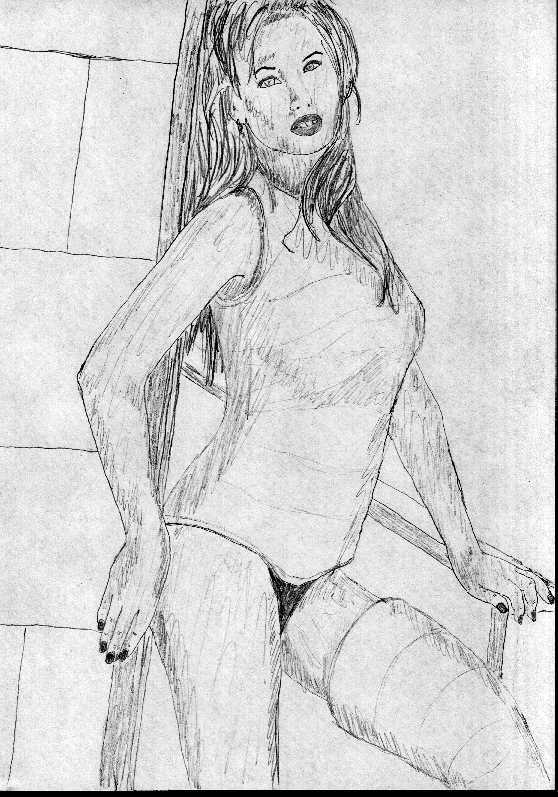
\includegraphics{images/kicks11.jpg}
\end{center}

\chapter{Dinner}
Sunday morning, I awoke feeling peculiar. It was that strange ``did I just dream that, or did
it really happen?'' feeling I get after a day where something odd happens. I shook the sleep out
of my head, and realized that the previous day had indeed happened as I remembered.

Dinner with Monique had been enjoyable to a point. Nothing fancy, we had burgers and beers
at a local pub.

The conversation was interesting, to say the least. We traded some very basic personal info.
I had to make most of mine up on the fly to conceal the facts about me, and hers was very
interesting: Some of it, I had already heard. She was born in Paris to a French father and
Vietnamese mother. She lived there until she was 8 years old, when they moved to Pittsburgh. Her
father died when she was 14, and she and her mother had a rough time of things ever since.

She came to this school studying education on a partial scholarship, but was working to pay
the rest of the expenses. The thought of her wanting to be a teacher was a surprise, since
teaching is not an occupation that would be the first choice of someone that was highly
materialistic.

Her conversation turned shortly to casts. She wanted to know more about the casts she had
just worn- what sort of injuries they treated. She also asked about casts that she had seen that
were in colors other than white, so I explained fiberglass vs. plaster to her. I even touched on
the strong and weak points of each. She asked if I ever used fiberglass, and I told her I did.

It was truly bizarre, being questioned in depth about casts and casting by a beautiful woman
who seemed quite interested in the whole concept. I reminded myself that this was a beautiful
woman who also had a cold and calculating side to her, with too much fondness for money, and
that's when it dawned on me- She didn't have any other interest in casts besides the money she
could make wearing them. Of course, had to be it! She really didn't care about casting, only the
money that it brought her. Hell, maybe she hoped to meet the ``man behind this,'' and get closer
to the money. Stupid me- for a short time, I was wondering if she really might like it. After
that, my answers became a little shorter, though not rude, and I was glad to take her home when
we were through.

Now, dressed and downstairs, I attack the mess from the day before. Two cutoff casts, in
Monique's well proportioned shape, and a lot of bandage wrappers and plaster drips. Still, it
was well worth it.

Monique woke up in a similar state of mind. She had to pause to recollect whether the
memories she had were dreams or reality. A quick feel into the pocket of her shorts was all she
needed. The money was there. Thankfully. Yes, she needed the cash; of that there was no doubt.
But she could no longer deny to herself that she did it only for the cash.

You liked it, and you know it. She thought to herself. You enjoyed the whole day, from the
casts, to the company. God only knows why- it is most certainly NOT right, but you did, just the
same. You enjoyed having those casts put on, you enjoyed them once they were set, you enjoyed
dinner afterwards, and you enjoyed who you did it with. But, did I really enjoy everything? Did
you really enjoy the casts, or did you just enjoy Quinn's company? Did you really enjoy Quinn's
company, or was it just that the casts made a profound impact on you that you naturally enjoy
him, since he introduced you to it?

Deciding that these questions were too much to think about, and that she didn't have an
answer anyway, she got showered and dressed. Still thinking about the previous night, she
decided to follow the impulses a bit longer, at least until she put them out of the front of her
mind.

Diane, her roommate who had first told her about Quinn, was still asleep upstairs, probably
not alone, either. Diane was emotionally weak, and never felt complete unless she was in some
sort of relationship, even if it was a bad one. Monique decided to take a few minutes to try
something on the computer.

She logged on to the Internet, pulled up a search engine, and entered ``plaster cast'' in the
search field. Most of the results were not of much interest, but one stuck out: ``Plaster of
paradise- resource page for those who want to wear casts'' her heart jumped a beat as she read
the words. She clicked the link, and was introduced into a world she would never have dreamed of
only a few weeks ago. She saw pictures, stories, anecdotes and other information, all by, and to
people who had an interest in wearing casts or seeing other people casted. She surfed the sites
for a couple of hours, until she was no longer the only one in then house awake. She excused
herself, and went out for a walk.

Walking in the warm morning air, her thoughts churned. She thought of some of the things she
had read and seen. She thought of some of the casts that looked interesting to her, and some of
the stories, both true and fictional, about wearing casts. Some of the casts looked like fun,
and some looked a bit too intense. She thought about how it would feel to wear some of those
casts, and the thoughts stirred heat within her. She definitely wanted to wear some of these
casts, and she wanted Quinn to be the one to put them on her. She thought of turning for home,
and calling Quinn and telling him the truth, and hoping he would (could) agree to cast her
again, maybe even today.

You really have lost it, haven't you? Just take down every defense you have, when you have
seen that this guy has his moody streaks. Sometimes he is warm and friendly, while other times
it almost seems like he can barely stand to be around you. Maybe that is part of the attraction
you have to him. He doesn't fawn all over himself because of the way you look.

Well, at least one thing is nice- you did finally admit that you ARE attracted to him. But
you can't call him again- not now, anyway. Maybe in a week or two, before summer session begins.
Unless you come to your senses and realize what a bad idea it is first. Maybe you should just
run from this. Better a little hurt now than a lot of hurt later.

Monique's feelings were torn down the middle as she walked aimlessly for the rest of the
morning, and part of the afternoon.

\chapter{}

\chapter{A New Direction}
What to do? I knew I needed something more from casting, but I wasn't sure exactly what that
was. I had taken my last two models outside while casted, and that certainly was pleasing, so
maybe that was a move in the right direction.

Maybe more casts per model, or bigger casts might be the answer. I have always loved body
casts, as well as multiple casts on a woman. The times I have done this have without a doubt
been my favorites. I have always liked the idea of a hip spica and shoulder spica combo, but
that would require getting very close to some very personal areas, and that really might be too
much to ask of a model. A model with all four limbs casted would be nice, too.

Maybe I wanted more realistic settings, such as having a model stay in the wheelchair for
photos and sketch. Perhaps crutches. Or maybe a hospital bed. That thought gave me an idea.

I went to the phone, and called my contact at the medical supply house back east. He said he
could get me the type of bed I wanted, as well as my list of accessories, but that he could not
ship it, as this type of bed was usually only sold to institutions, and not private individuals.

I told him to have it ready in two days, and I would have it picked up. I then called an
interstate mover, and arranged for them to pick it up, and deliver it to me. I claimed I was
helping a relative convalesce after an accident. With the cover story in place, all was in
motion.

I decided to convert the downstairs bedroom that had previously served as my den into a
makeshift hospital room. I spent the next two days moving things out, and painting the room
white, so that it would look correct. My phone hadn't been ringing with new models much lately,
so I wondered if I might be acting a bit hastily. I really liked this little town, but with the
school semester ending, and summer break beginning, I might lose a lot of my potential models. I
decided to try something different to see if I could get things rolling.

I called the office of Kicks, and told them the changes I wanted to make to my ad. The ad
now read: ``Part-time summer modeling work for adventurous women. Full-time pay for one day's
work. No nudity, but an open mind is required. Steady weekly work through the summer.'' My plan
was simple- find two or three models that I could work with on a weekly basis throughout the
summer.

\begin{thought}
It was finals week, and Monique had been studying hard. It had been difficult, as she had
been spending as much time as she could on the Internet, looking at casting websites. When she
wasn't online, she was looking forward to getting back to the sites. Since she had found the
website that dealt with casting, and those who enjoyed it, she had been strongly drawn to this
dark little corner of cyberspace. After a week of surfing, she felt she had finally made it
through all of the sites.

Most of the sites were mainly pictures (mostly of women) wearing different casts. She
pictured herself wearing many of the casts she saw, imagining what it would feel like to have
the cast applied, and what it would feel like once it was set. She found information about the
casting process, though she already knew quite a bit about it from watching Quinn as he casted
her. She learned a bit of history, how casts as treatments are getting rarer and rarer, and how
fiberglass had almost, but not totally, superceded plaster for the most part.

But, what fascinated her most were the stories, both real and imagined involving casting and
why people were attracted to it. Many people enjoyed wearing the casts for the restriction they
offered. She could relate to that, though she knew that was not her only reason for liking it.
She was fascinated to read that some liked casts for the attention they draw from strangers when
worn in public. The idea of wearing a fake cast in public astounded her. What if she saw someone
she knew? Someone who knew she wasn't really injured. The possibility of getting caught was bad,
but the idea still held allure for her.

Yes, Monique had admitted to herself that she liked wearing the casts she had worn, and she
wanted to wear more. She had even considered ordering some supplies, and casting herself, but
expenses and a roommate made that less than feasible. Besides, (and this was the part she still
had trouble with) she really liked Quinn, and liked when he casted her. The thought of doing it
herself just didn't seem as nice as having it done for her.

That presented a new dilemma in itself: She couldn't approach him to tell him al of this,
yet she wondered if she could go much longer WITHOUT telling him. For the meantime, she would
concentrate as best she could, and maybe calls Quinn next week, after finals were over. Until
then, she would try to sate the desires by examining the photos, and imagining what the casts
must be like. She definitely already had an idea of several things she wanted to try.
\end{thought}

Erin had a problem. She needed money to pay the rent, but she wasn't working, and though her
job was waiting for her she couldn't go back for a while. She had a great job at a factory, but
working wasn't possible for several weeks yet, and the rent still came due. If she couldn't come
up with the rent, she'd have to move back home, and that was simply not an option she wanted to
go with. She had left home two years ago after a huge argument with her parents. She just
couldn't live with their rules, and she refused to go to college, as they demanded. Now, her
independence had hit a snag, and was in jeopardy.

She re-read the newspaper ad: ``Full time pay for one day's work.'' That definitely would
work, if they would take her as a model. She decided to call. She had the open mind they asked
for, and if they wanted attractive young women, she should definitely fit their needs. Her
condition would probably exclude her, but if this modeling was from the waist up, she'd be OK.

My phone rang

``Hello?''

``I'm calling about your ad for models. What sort of models do you want, and what exactly
would I be modeling?''

``Well, we're looking for attractive ladies at least 18 years old, and the nature of the
work is best explained in person.''

Erin thought on this one for a bit. She was old enough at 20, yet still young. And she was
sure she was attractive enough.

``Well, I guess we could meet and you could decide if you want to work with me.''

I told her that would be fine. We arranged to meet in an hour, since she was free that day,
and I was working on preparing my ``hospital room.'' I grabbed a quick shower, and waited for
her to arrive. I went into my ``hospital room'' in progress, and admired what was there. The bed
was very cool, with its assortment of traction and other orthopedic attachments. This would be a
very cool backdrop for photos. As I looked things over, there was a knock at the door.

I opened the door to a very beautiful young woman. She was certainly young, 20 at the most,
with long red hair, beautiful blue eyes, and a stunning figure. She wore a black dress with
sheer see through panels around the neck, midsection, and lower skirt. It was clear she had
dressed to impress me, and she had. She had a fantastic tan, especially for a redhead, and I
wondered if the red hair might come from a bottle, as if it mattered. What really floored me
most were her legs. Her left leg was long, wonderfully shaped, and very tan. Her right leg was
in a pink long leg cast!

\chapter{~}
``Hi, I'm Erin.'' Said the girl in the long leg cast.

My heart was pounding. I've seen some very attractive women around this town, and I've had
the good fortune to see several of them in casts, by my own hand. But something was different
with this one. I wasn't sure if it was her cast, or her breathtaking beauty that was affecting
me that way. Another part of my mind found humor in the irony- I was seeking women to cast, and
this one comes with a cast of her own.

``Come inside, Erin,'' I said. I led her to the parlor, and pointed to the couch and asked
her to have a seat. Thinking of her leg, I excused myself long enough to retrieve one of my
stands from the casting room. I made these stands to support a leg during the casting process,
it should help her be more comfortable.

``Here, try this for the leg,'' I told her and she hoisted her leg into the cradle. It was
very exciting, to watch her managing with her leg being stiff and heavy, and I could have easily
lost myself in that moment, but I forced myself to remain professional.

``Comfortable?'' I asked.

``Yes, I have no idea what this thing is, but it works great for sitting down with this
cast.''


``So, what happened to your leg?'' I asked.

``Well, I was doing some painting in my apartment, and I leaned a little too far on the
ladder and fell. When I came down, I landed off balance on my leg, and I heard a snap. They
showed me the picture of my leg, it broke right about here.'' She made a motion with her hand
about 4 inches up from her ankle. ``So now, I'm stuck in this cast, and I guess I should have
told you before I came. If this modeling isn't from the waist up, you have no use for a woman
with a broken leg.''

``Erin, your leg does not exclude you from this job. In fact, it is a benefit. Remember when
I said you'd need an open mind for this job?''

``Yes,'' she said, with obvious unease in her voice.

I decided to cut to the chase. A cast fetish will probably disgust her, since she is forced
to wear a cast for weeks, and it's obviously a major inconvenience for her. But, if it does,
best to know it early.

``Erin there are people out there who are attracted to things far outside the realm of what
is considered normal. Some are attracted to things that are bizarre.''

She had a troubled look on her face, and I was sure this was going to end badly, but I
pressed on. ``There is a fairly large group who are very excited by seeing a woman in a cast.''

Her eyes furrowed as she blurted out ``You mean there are perverts out there who get their
jollies from the pain I went through?!''

``No, I don't know of any who are turned on by the pain or suffering. The ones I know of are
simply excited by the cast.''

I was trying to calm her down, even if this whole thing turned out to be a wash. ``I have
heard several theories on the subject, some think that the perceived vulnerability is what does
it. Others think it is the extra care that a person challenged by an injury would need. For
some, it is simply a bondage issue. Some think it may be a combination of these, but nobody
claims that they like it because of the pain and suffering. Mainly, the audience I work for is
adamant that he does not enjoy the injury, only the cast. In fact, he feels a bit of guilt over
the fact that what turns him on is a byproduct of an injury to someone else. That's why he hired
me.''

She still looked upset, but maybe not as much as she was.

``And what exactly is it that you do for him?'' She asked.

``I am an artist and photographer,'' I replied. ``I provide him with photos and sketches of
beautiful women in casts. Since it is not everyday that you find a woman in a cast, I apply
casts to women, and they serve as models for my work.''

``This is weird. Too weird. So how did you come to this? What made you this way?''

For a moment, I considered telling her the truth. Her beauty and emotional strength were
extremely alluring to me. Maybe. Maybe it was just the cast. I decided to stick to the stock
story. I explained that I was just hired help, too. Hired by a wealthy man who wished to keep
his identity secret, for obvious reasons. He was the one who financed all of this, and while I
appreciated female beauty, the casts really did nothing for me.

``Strange way to make a living.'' She spouted.

``Yes, but better than having to try to do more mainstream art, and make a living doing the
same thing as thousands of other artists. And it sure beats holding down a nine to five job. In
addition, not only do I have this great house for a studio, but I get to live here rent free.''

``Good point,'' she said. ``It is a cool place.'' She seemed to be softening, but I wanted
to find out.

``Anyway, in case you might still have any interest, here is the proposal: I need two or
three models to work one or two days per week. On the day you work, you would start at 9:00 am.
You will be placed on a cast, or maybe more than one. After they set, I will photograph you, and
then do a sketch of you. After that, you will be cut out of your casts; (minus the one you came
in with, in your case) paid, and sent home by 5:00 p.m. Some days, I might want to start a bit
later, but I would let you know in advance. The pay is in cash, and we obviously want
discretion- we would prefer you don't tell anyone about this.

``This is unbelievable,'' She said. ``Here, I'd give anything to be rid of this cast, and
yet I'm being asked to wear more of them.''

``I know it seems really odd, but you don't have to decide now. Also, if you try it, and
find that you don't want to continue, you can stop at any time, even if it is in the middle of a
session. And, we do pay well.''

``How well?''

``We graduate the pay based on exactly how you are casted. The lowest pay we have is two
hundred dollars, which would be for a below the knee cast on your leg, or a below the elbow arm
cast. The highest paying cast would be six to seven hundred dollars, but to get there, we'd be
talking about a body cast, maybe with an arm or leg included. Maybe I can arrange for a bit
extra for the cast you'll be bringing with you.''

This is really freaky. I need to make some money, since I can't work with my leg like this,
but I just don't know. Can I think about it awhile and call you?''

I wanted to prod her to say yes, but knew that was a bad idea. ``Absolutely.'' I told her.
``I need two or three, maybe even four models, and I have one strong candidate already. I'm
offering the second spot to you. If you decide to take it, it's yours as long as it is still
open.'' There- not forceful but hopefully giving her a sense of urgency.

``Fair enough.'' She replied. I won't take too long to decide, and if the job is gone, then
I'll know it wasn't for me.'' She lifted her leg out of the stand, and lifted herself up with
her crutches. I showed her to the door, and watched her hobble down the walk on her crutches.

I went to the parlor and lit a cigarette. I really hoped she'd take the job. I really wanted
to cast her, and I wanted to do it more than once. I wasn't sure if it was her or her cast, but
I wanted to cast her more than any of the women I had casted already. I got up and went to
finish the painting in the new ``hospital room,'' still thinking about the woman I had just
interviewed.

The phone interrupted my work.

``Hello.''

``Hi Quinn, it's Monique.''

``Hi Monique. What's up?''

``I have something I need to talk to you about. Can I come over?''

``I guess so.''

``Great, I'll be there in half an hour.''

\chapter{}

\chapter{~}
Tuesday had been eventful. I had met the most exciting woman I had seen in a long time,
maybe ever. She was considering being a cast model for me. I could not deny to myself how much I
hoped she would accept. Nor was I kidding myself that possibly I wanted more than just to cast
her.

I had also established one regular cast model, even if it was Monique. Besides, Monique was
very beautiful, despite her personality. I tried to figure her out. I wondered why she was so
eager to accept the higher involvement casting without even asking about the increased pay. I
would have figured she would be all over that. It didn't make any sense at all until it occurred
to me that she was likely angling to get past me, and straight to the fictitious ``money man.''
By appearing enthusiastic maybe she hoped to get more attention, maybe have the rich sponsor
want to meet her, and then let her physical attributes work their charm. Ugh, as ugly as it
sounded, that had to be it. Well, maybe I'll work with her until I establish a couple more
models, then cut her loose. I'll tell her that the man in charge has no further interest in
seeing her casted. That will put her in her place. But for now, casting Monique is a lot better
than casting nobody, so I'll roll with it for a while.

\begin{thought}
Monique still could hardly believe what she'd heard the day before. More casts? Bigger
casts? Public?! This was too good to be true! What Quinn proposed was exactly what she had been
wanting! It was a shame that Quinn wasn't more into this himself. Though it was just a job to
him, it was a life she was liking more and more all the time. It was probably best that he
wasn't truly a ``caster,'' though. She was having enough trouble keeping up her normally iron
clad self control anyway, if he was really into it, she might end up throwing herself at him and
messing everything up. She was obviously letting her newfound fascination with wearing casts get
the best of her emotions. She reminded herself: ``Remember, Monique- this is just a job to
Quinn, and he thinks it's just a job to you, too.''
\end{thought}

My phone rang, and to my pleasant surprise, it was Erin.

``Hello, Quinn. If the job is still open, I'll take it.''

I was ecstatic, but hid it. ``It is still open.'' I told her. ``I'm glad you've accepted. I
think I'll enjoy working with you.''

``Well, I'll be honest with you, this wierds me out, but I need to make some money. I can't
promise that I'll do it any longer than it takes for my leg to heal. I have a good job, and
they're holding it for me, but I need to pay my rent in the meantime.''

``I understand,'' I said. Her words disappointed me a bit, but they were understandable.
Besides, even if it was only once, I wanted to cast her! I hoped that maybe she would find it
not so bad when it was temporary, and not accompanied by pain. Sure, that was a longshot, but
some women actually enjoyed being casted, though I doubted the likelihood that I'd ever meet
one.

``When do we get started?'' she asked.

``How about Monday? In fact, we could make that our normal day.''

``You said I'd be paid in cash the day of the work, right?''

``Yes''

``Then Monday will be fine. And if I decide to do this any more after the first time, we can
always work on Mondays. My schedule is really pretty open.'' She said.

``Also, we can work around conflict, if we need to,'' I added.

``Ok, we'll do this Monday. I'll try it, and then decide if I want to do it again. Is that
OK?''

``Absolutely, but only if you're comfortable.''

``Thanks. Oh, what should I wear? Besides my cast, that is.''

I gave her a rough outline of the type of clothing I wanted, and she said she had some
different things that might work, and she'd bring a selection with her. We said our good-byes,
and I as faced with a pleasant dilemma: how did I want to cast her? I could think of a lot of
ways I WANTED to, but I didn't want to overwhelm her, and scare her away. I wanted to cast her
more than once.

While I pondered how to ``dress'' Erin, I decided to call Monique, and get her scheduled,
too. I told her I'd like to cast her on Fridays, starting a week from the one coming. She
sounded eager when she accepted.

``Sure, Quinn. What sort of cast will I get this time?''

``Well, I don't know yet. I'll talk to the boss, and see if there's anything particular he'd
like to see you in.''

Her next statement floored me:

``Well, if he doesn't have anything in mind, I can help you decide if you need me to.''

\chapter{~}
Monday morning at 9:00, Erin crutched up my sidewalk looking great. She wore denim shorts,
red T-shirt, and a sandal on her right foot. Over her shoulder was a small overnight bag, no
doubt with part of her wardrobe for the session. Of course, the rest of it, I would be
providing. I met her at the door.

She smiled. ``Well, here I am, ready to go, I think.''

``Great. Come on in and we'll get started,'' I said, trying to hide my excitement. ``May I
take that bag for you?''

``That's OK, I've got it,'' she said, not trying to hide annoyance. ``My leg is broken, not
my arm.'' Sort of a bitchy answer, but she probably was getting sick of being treated like an
invalid.

I led her to the casting room, where I had everything ready. I asked her to have a seat for
a few minutes before we started.

``Erin, I'm really glad you have decided to try this. I spoke to the ‘Boss,' if you will,
and he's eager to see what sort of work you and I can turn out.''

``Well, it sounds like my part will be pretty easy- just sort of sit back and let things
happen,'' she said.

``For the most part, yes.'' I told her. ``But your attitude can really show through in the
work, too. It will affect the final work.''

She smiled again. ``I won't let you down.''

``I'm sure you won't.'' I thought to myself.

``For today, Erin, I don't want to do anything overwhelming. I'd just like to do a quick
shoot here at the studio. We're not going to cast you too heavily, either. I think for your
first time, we'll just put a cast on your right leg like the one you already have.''

``Sounds fine to me,'' she replied.

``Did you bring tasteful lingerie, like I asked?''

She nodded, and opened up her bag. She removed the items one at a time and my mind raced as
I saw each item and pictured her in it. When the bag was empty, she asked which one I liked the
best. I honestly could not decide- I wanted to see her in all of them.

After a quick moment of thought, I told her ``How about you wear whatever you're most
comfortable in?''

Now it was her turn to think for a moment. ``I think that would be these,'' she said,
holding up the simple dark blue camisole set.

``OK, I'll leave you to change. But first, your pay for today will be \$350.00, and we
should be done by 1:00 p.m. I handed her the envelope, and left her to change.

Out of the casting room, I went into the ``hospital room'' which still smelled of the white
paint I had finished the day before. I retrieved the wheelchair, then went and filled my bucket
with warm water. I was nervous, and I knew why: All of the women I had casted were very
attractive, but Erin was different. Maybe it was her cast, but I didn't think that was it. There
was something more than the cast, and her beauty that was pulling at me. I decided to smoke a
cigarette to calm myself. She might need a few extra minutes to change, anyway, considering she
had to fight with a long leg cast.

I returned to the casting room and tapped lightly on the door. ``Are you ready?''

``Yeah. Come on in.''

I went inside, and was very pleased at the sight I beheld. She sat on the casting table, and
in the dark blue lingerie and hot pink cast, she looked fantastic. Once again, I had to remind
myself to stick to the program, and appear professional.

``Well, it looks like you're ready to start, so let's begin.''

``Ready as I'll ever be, go ahead,'' she replied.

I took the roll of 4'' wide stockinette, and unrolled what I knew from experience to be more
than enough. I slid it up her right leg to her upper thigh. I didn't go quite as high as I would
have liked, because I wanted the cast on this leg to match the other one. I then started the
padding from the top and worked down, smoothing out the bunches in the padding as I made each
turn.

``So, am I doing it the same way as the pros?'' I asked, trying to make some conversation.

``I really don't remember when they put the cast on,'' she said. ``They had me pumped full
of Demerol, and by the time they put the cast on, I was pretty well out of it.''

I gave her an understanding nod as I ripped open the first roll of 4'' pink fiberglass.
Working in the same downward motion, I had used six rolls of fiber before the cast was finished.
I pulled off my gloves.

``There' we'll give that a few minutes to set before we go into the other room,'' I engaged
her in some small talk, just trying to make conversation, to pass the time. She was polite, but
didn't seem too eager to talk about herself- her job her friends (never mentioned a boyfriend, I
noticed) or her injury. Her broken leg disgusted her, and by the way she looked at it, she
wasn't too happy about her new cast, either. Hopefully, she would warm up to it, even if only a
little.

When more than enough time had passed for the cast to set, I told her that it was time to
move to the other room. She reached for her crutches, then looked at me: ``Will this work?'' She
asked.

``Probably not, I have an easier way.'' I stepped out of the room, and pushed the wheelchair
inside.

``Here, grab around my neck.'' She did, and I lifted her up and placed her gently in the
wheelchair. I must tell you, that was a pretty intense experience for me- a definite dream come
true. I was helping an extremely attractive woman in two leg casts get into a wheelchair, it was
almost hard to believe. I adjusted the leg rests to accommodate her legs, and pushed her into
the ``hospital room.''

I took a few photos of her in the wheelchair. She put on a nice smile, and looked wonderful,
but the smile seemed very ``pasted on'' to me. I really wished she had been a little more into
the photos.

I helped her onto the bed (Wonderful again), and took some photos of her from various
angles. Once I was ready to do the sketch, I had the idea for her to close her eyes, and act as
though she were asleep. With her eyes closed, I felt a little freer to admire her beauty as my
pencil worked over the paper. It almost amazed me, watching her image take shape on the page in
front of me.

When I was done, I said ``There- all done,'' and showed her the drawing.

``Wow, that really looks like me!'' she said.

``Thank you. Are you ready to get out?''

``Yes!'' She said, a little too eager for my taste.

``OK, back to the other room.''

I picked her up from the bed and placed her into the wheelchair once again, then back onto
the casting table once we were back in the casting room. I remember thinking to myself that I
could really get used to it.

Once back on the table, I took the cast saw and carefully cut down the sides of the cast on
her right leg. When the cuts were done, I used my bandage scissors to cut the padding \&
stockinette on the outside of the leg. The cast opened up, and Erin pulled her leg out.

``I don't suppose I could talk you into doing that to this one could I?'' she said, tapping
the cast on her left leg.

``No, and you really don't want that anyway,'' I replied. ``As much of a pain as it is, that
cast is your leg's best friend right now.''

``Yeah, yeah- I know, but it's hard to remember that sometimes. Have you ever had to wear a
cast?'' She asked, reaching for her shirt and shorts.

``No, I told her. Of course, I had casted myself several times, but had never been forced to
wear one for an extended period of time. I could easily understand the inconvenience of having
to wear one for weeks.

``Well, let me tell you, it's no picnic.''

``I can imagine so. Let me get out of here while you dress.''

``That's OK, I'll just put my clothes on over these,'' she said, bending to get her shorts
over her casted left foot. Watching her dress, I knew I had to make some sort of conversation,
even if it was lame. Otherwise, I would simply be ogling her, and I didn't want to scare her
away.

``So, what do you think of the modeling job?'' I asked.

``It's really weird.'' She replied.

I was a bit dismayed. ``So, do I need to find a new model for Mondays?''

``No, I don't think so. It's weird, but it pays well, and I don't see anything wrong with
it,'' She said as she pulled on her T-shirt, and bent to put her sandal back on her right foot.
She hopped down on her right leg, and grabbed her crutches. With a smile she added, ``As long as
I'm still welcome, I'll be back next week.''

``I'm sure you will be.''

``Then I'll se you next Monday at 9:00?''

``I'll be looking forward to it,'' I said before realizing how it sounded.

She looked at me a bit oddly as she crutched past me to the front door and let herself out
before I could open the door for her. I peered out the window as she hobbled down the walk,
lowered herself into her car and drove off.

Amazing woman.

\newpage
\begin{center}
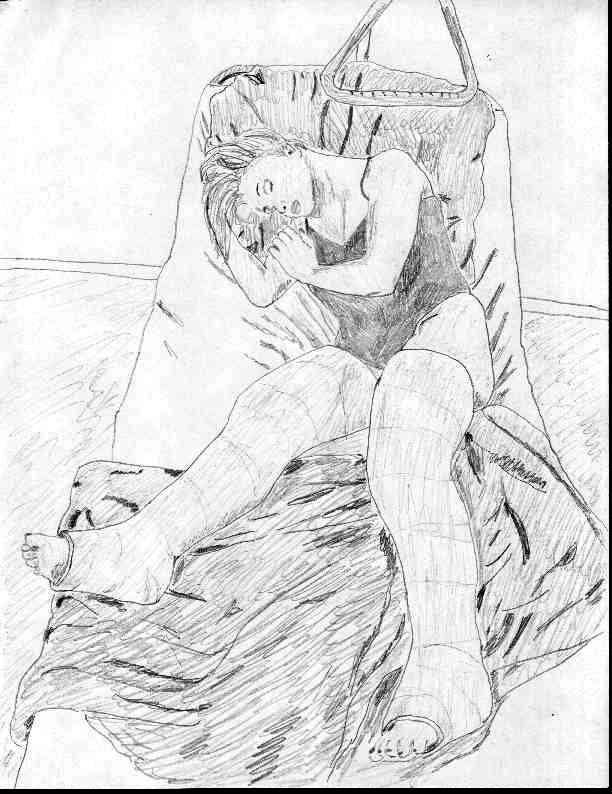
\includegraphics{images/kicks18.jpg}
\end{center}

\chapter{~}
Detective Cassidy Smith sat at her desk, looking over a report one last time before she
turned it in. She hated paperwork, but she loved being a cop. She'd wanted to be a Police
officer since she was a little girl. She'd done well in school, and her parents had cringed when
she had told them her college major was going to be Criminology, with a Psychology minor.

After graduation, she'd come to this town, and had made Detective after only two years. Now,
at age 26, she had more decorations and commendations than most officers at retirement's door.
She also had the respect of the officers she worked with, despite her gender, age and looks.

Detective Johnson walked in. ``Hi, Cass. How's it going?''

``Fine. What's up?''

Cassidy liked working with Tom Johnson. He was smart, and tough- the kind of guy you wanted
with you in a tight spot. Last year, they'd worked together to catch a lowlife who'd been
abducting, raping and beating young women. Cassidy had been the bait, and when the scumbag had
gone for her, Johnson had closed in so fast; the guy never knew what had hit him. Johnson was
also very dedicated to his family: an all- around admirable guy.

``What's the project, Tom?''

``Young women see ads for models in newspaper. They call, they go, guy seems nice, share a
soda or beer, take some pictures, next thing they know, they're waking up, having slept with the
guy, but not remembering it.

``Drugged.''

``Yep- Ketamine Hydrochloride in every case.''

``Good old Special K- it never gets old,'' she said.

``Here's the kicker- look at the locations: Small college town near Detroit, small college
town near Chicago, small college town near Indianapolis. Do you see a pattern, here?''

``Yeah,'' she said. ``It looks like he's moving. Our way, no less.''

``He likes college girls, and we're right in the path of destruction,'' Johnson said.

``So, let me guess,'' Cassidy said. ``I'm going back to school?''

Johnson smiled. ``No better way to catch a fly than with sugar.''

``Oh, my- I believe I've just been a victim of sexual harassment, Cass said, joking.

``Yeah, sure, and if I'd really harassed you, I'd probably be spitting out teeth right
now.''

``Violence?'' Cassidy asked, batting her eyes. ``From sugar such as I?''

``Yeah- whatever. Anyway, take a look at this. He tossed down a copy of Kicks, opened to the
ad section. Cassidy read aloud the ad that Johnson had circled:

``Models wanted no experience necessary. Week's pay for a day's work. No nudity, but an open
mind is required.'' She handed it back to Johnson. ``We need to call the paper and see what they
can tell us about the person who bought this ad.

Johnson was ready. ``The guy's name is Quinn, he doesn't show priors in any database, and
doesn't have a driver's license in this state. They're still checking on other states. The paper
also said that this is the first week that the ad has run.''

``Then I guess it's time to give this Quinn a call, and see just what he wants with
inexperienced models,'' Cass replied.

``Go ahead and call. We've already established the same cover at the college that we used
last year.''

``Pretty bold of you, doing that before you even asked me if I wanted in,'' she said,
turning to her desk, opening a drawer in search of a file.

``I know you Cass- you live for this kind of stuff. Going under to catch a dirtbag is fun to
you. I knew you'd want in, and I knew you would probably want to start right away.''

``Yeah, yeah- you're lucky you have me, all I have is you.'' She found the file she was
looking for- it had the details of fictitious college junior Samantha Cassidy: Age 21, Drama
major, and Psych minor. Class schedule, as well as other minor details that Cassidy would have
to learn again.

``Whatever, 'Sam.' Just make the call.''

``Yes sir!'' she said with a salute as she punched the button on her phone for the secure
line.

\chapter{}

\chapter{}
Monday morning at 9:00, there was a much anticipated knock at my door.

I opened the door to see Erin, looking just as beautiful as I remembered. She was wearing a
very nice dark gray evening dress that was very flattering. I wasn't sure, but I thought that
the pump she wore on her right foot was a Prada. She really liked to dress nicely, even if the
dress was really a bit excessive to wear in the morning.

``Good morning,'' she said with a smile. ``May I come in?''

``Absolutely,'' I said, holding the door open while she crutched through.

We headed to the parlor. I sat on the chair, while she sat on the couch and lifted her
casted left leg onto the couch.

``How's the leg?'' I asked.

``Healing, according to my doctor. He says if things keep going the way they are, I may get
a new cast soon- a below the knee cast, and maybe even be able to walk on it. Getting rid of
these crutches will be a VERY happy day for me.''

``I can only imagine,'' I said, enjoying the conversation.

``Maybe there's more to this… thing… with the casts than I thought. Since we first talked,
it seems like everywhere I go; everyone seems to stare at me.''

That one got me going. ``Well, that's probably true to some extent, but you also have to
consider that you may be hypersensitive, given your inconvenience over the injury. Then, add in
the fact that you're now aware that there are people interested in casts, and you're probably
really noticing yourself being noticed. Also, as attractive as you are, you probably turn a lot
of heads anyway.''

She smiled at that. ``Thank you. Now, on the phone, you said something about a cast on my
arm this time.''

I was a bit disappointed at her change of the conversation. I explained the long arm cast to
her again. We then headed to the casting room. She opened her overnight bag, and started to show
the lingerie she'd brought, but I stopped her.

``Erin, that dress really looks nice, let's just leave you in that. We'll cover it up to
protect it while we put the cast on.''

``OK,'' she responded.

I took the bucket to fill. While it was filling, I got the envelope with her cash that I had
already prepared. When I returned to the casting room, I set the bucket on the cart with the
rest of the supplies, and handed her the envelope. She opened the envelope, thumbed through the
cash, and put it in her purse.

``This is really easy money,'' she said. ``Way bizarre, but easy.''

``Well,'' I replied, ``there are no promises, but you should be able to do it for a while,
if you like.''

``I'll think about it,'' she said.

I certainly hoped she decided to continue casting after her leg was healed. I knew she was
pretty well irritated by her cast, but did this because she needed to make money while she was
off from work with her leg. She seemed rather chilly, but I also found myself hoping that traced
back to the leg injury, too. I liked Erin. I was very attracted to her, and hoped maybe she'd
open a door for me to ask her out at some point. For the moment, I had to calm myself. Although
I was pretty cool and businesslike on the outside, (or at least hoped so) I was very excited
about casting her, and could feel my heart beating faster than normal.

I took a sheet of plastic drop cloth, and wrapped it around her, under the left arm, and
over the right shoulder.

``That should protect the dress.''

She nodded, and I continued. I took the roll of three inch stockinette, and cut off a piece
about four feet long. She held out her left arm, and I slid the stockinette up to her shoulder,
bunching it a bit at the top. I took my scissors, and made a small slit over the base of her
thumb, then pulled her thumb through the opening. I completed the stockinette by cutting it off
flush with the second knuckle of her middle finger. I then started the padding. I wrapped the
hand and wrist with one inch padding, being careful not to get it too thick. Hands are the
trickiest body part to cast, and make it look well. It's very easy to get the padding of the
casting tape too thick. After the hand and wrist were padded, I started just below the shoulder
with three inch padding and worked down, making sure to make an extra turn at the elbow to
protect the bony area there.

I pulled on gloves, and ripped open a roll of two inch pink fiberglass. I took Erin's padded
hand in mine, and turned it so the palm was facing upwards. I told her to hold the position for
me, and then dipped and wrung out the roll. I began wrapping her hand in a figure eight pattern.
As the turns passed between her thumb and forefinger, I folded the tape in half, so that the
cast would allow movement of the thumb and not ride up the finger. I also made sure to keep the
tape from getting too thick. Erin was very beautiful, and I wanted her cast to be beautiful,
too.

After the hand and wrist were wrapped with the roll of one inch fiberglass, I used three
inch rolls to complete the cast, working from the top of the cast down to the wrist, casting her
elbow with a ninety degree bend. When I was finished wrapping, I rubbed smooth a couple of
areas, then pulled off my gloves and tossed them into the trash. I took a towel and blotted the
droplets of water that sweated up on the surface of the cast.

``Just hold it still for a few minutes, and it will be set. Do you want anything to drink
while we're waiting?''

``Sure. Do you have any bottled water?'' she asked.

``I think I do, let me go check.''

I went to the refrigerator, and got her water and a soda for myself. When I returned to
Erin, I took the plastic off of her, and handed her the water. To my pleasant surprise, she
started asking questions.

``So, how did you come to do this? She'd asked the question before, at our first meeting.

``Well, I'm just hired help like you, really.'' I answered.

``No- I mean, how did you get picked to do this? Did you answer an ad too?''

``No,'' I answered.'' Some of my work was on display, the right person saw it, and I was
approached.''

``This 'right person' is very secretive about his identity, isn't he?''

``Yes, he is. Between us, you'd know his name if you heard it.'' At least that wasn't a lie.

``Has he given you any feedback on our work?''

``He liked it.'' Again, I was telling the truth, even if there was a lie in it.

``When you first interviewed me, you mentioned that there might be some really big casts or
instances where I might wear more than two casts. Are you just starting me slowly, or is that
not in the works for me.''

That one floored me. ``We're purposely starting slowly. Since you have a broken leg for
real, and already have a cast inconveniencing you, we don't want to get too intense, and scare
you off.''

``I appreciate that.'' She said. ``But I'm okay with the bigger casts, if that's what is
wanted from me.'' Wow!

The conversation went on for a few more minutes before I suggested we head to the back porch
for the pictures. I helped her into the wheelchair, and took her to the porch. I took about
three rolls of pictures, some of her in the wheelchair, and some with her sitting on the patio
furniture. I really enjoyed taking the photos- the camera gave me an opportunity to take some
longer looks than I dared to do otherwise.

I finally decided on a pose in a chair for the drawing. Again, I enjoyed my opportunity to
stare at her while I was sketching. Admittedly, I took longer than necessary making the drawing.
I was a bit lost in the moment.

When I was finished, I took Erin back to the casting room, and got her out of the arm cast.
We said our goodbyes, and I told her to give me a call within a few days to plan out next
Monday. She agreed, and left, but not after flashing me that great smile of hers.

By the time I had taken her arm cast downstairs, I already had next Monday planned.

\newpage
\begin{center}
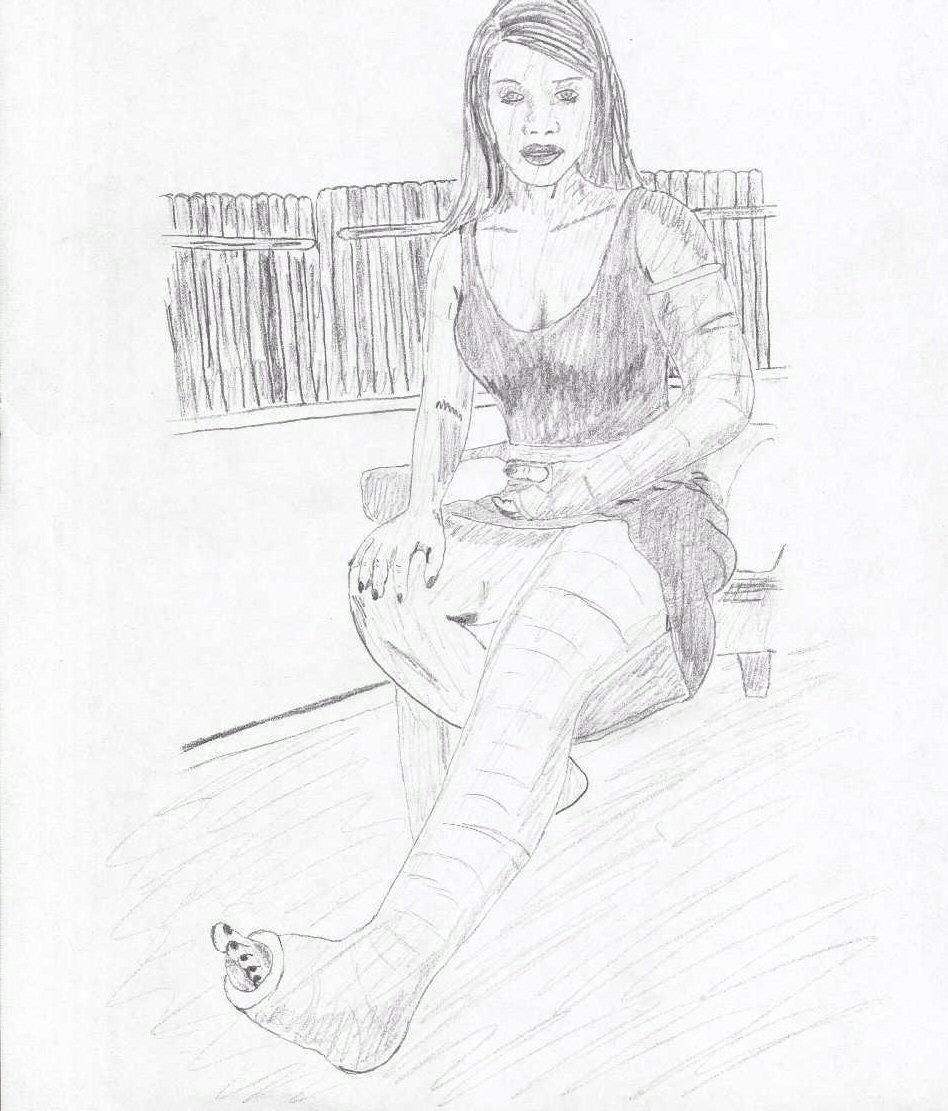
\includegraphics{images/kicks21.jpg}
\end{center}

\chapter{~}
Cassidy was nervous. Not in a way that hindered her ability to function, or even function
well. She was always nervous when working undercover. Setting a trap with herself as bait always
required making herself more vulnerable than any cop ever likes to be. Also, the very nature of
this work was bizarre, to say the least. She supposed that the nerves were probably a good
thing. If she got too comfortable working undercover, she might make a mistake, maybe a fatal
one.

She had a half hour before her meeting, and she and Johnson went over the plan one last
time. The technical officer had fitted her with a tiny microphone and receiver. It was so small;
it actually was hidden inside a fake hearing aid. Her hair covered her hears, but even if it was
seen, she had a story ready about being born with some hearing loss. The added benefit of this
type of setup is that it allowed the guys monitoring the conversation to talk to her, as well.
She also had a more sensitive microphone and transmitter hidden in her purse. This one would
pick up sounds within a 15 foot radius. The microphones were being monitored by separate
officers in a van parked half a block away from the suspect's house. The van had engineering
company markings, and there were even two additional officers outside the van who appeared to be
doing survey work. The van was already in place. Johnson would be in his car, a block away and
out of sight, but in constant radio communication with the officers in the van. Finally, there
were three additional officers in marked cars patrolling the area, able to assist within a
couple of minutes notice.

In the parking lot, Cassidy asked Johnson one last time: ``Why all of the undercover work
and expense? Tell me again why we didn't just go over and question this guy?''

Johnson sighed and smiled. ``Relax, Cass. We don't have any evidence that this guy is the
perp we're looking for. If we went in asking questions, we'd be treading a fine line with
harassment. If he IS our guy, with no evidence, we'd be likely to scare him off. Most likely,
he'd hurt some other woman before anyone picked up his trail again.''

``I know, I know. I just wanted to hear it again,'' Cassidy answered. ``This is just so
weird- posing for pictures in my underwear and a cast.''

``Highly weird.'' Johnson said. ``I know the cast worries you a bit, since it means you
won't be able to move as well in an emergency. That's why we have the extra patrols. Everyone
knows the situation, here. You say the panic word, and we come down on him like a ton of
bricks.''

``I trust all of you guys totally. Wish me luck.'' She said, getting into the department's
seven year old Toyota.

``Good luck, Cass. Just relax, and let's see if this is our scumbag. We're right
outside.'' Johnson said, shutting her door, and turning to his cruiser.

At 10:00am, a red Toyota pulled up and parked along the street in front of the house.
Samantha got out, looking as good as she had when I had met with her over the weekend to discuss
the modeling. Samantha was tall, probably about 5'10'', and very athletic. She was wearing a red
tank top, tight blue jeans and white tennis shoes. She opened the back door of the car, and got
a small duffel bag out of the back. When she bent to pick it up, a guy in a survey crew down the
road whistled at her. She scowled and jabbed her middle finger at him, and turned to the walk.

I let her inside, and we sat for a few minutes and talked before starting.

``So, you've never had a cast before, Samantha?''

``No, I've had several sprains, but I've never actually broken anything. And please, call
me Sam.''

Calling a beautiful woman 'Sam' seemed wrong to me. Sam was the butcher from ``The Brady
Bunch.'' But, if that was what she wanted, I guess I would.

``As I told you the other night, we'll be doing a small cast today. It's not really
indicative of what we'll be doing in the future, but it's a good place to start, especially
since you've never had a cast before. If you continue after today, we'll slowly progress to more
and bigger casts. Before we start, do you have any questions?''

``Just one: How do you take the cast off of me?'' Cass knew full well how a doctor removes
a cast. Despite the cover story, she had actually worn casts a few times. She had broken her arm
in a childhood fall, she'd broken an ankle while in high school, and had had her wrist broken
during an arrest a little over a year ago. She was asking mostly out of concern for her safety-
she didn't want this guy coming at her with a knife, or worse.

``I remove the cast the same way a doctor does,'' I told her. ``It's totally safe. Come on
into the casting room, and I'll show you.''

I led her into the casting room, and retrieved the cast saw from the cabinet. ``I know it
looks scary, but it cannot cut you.'' I plugged the saw in, turned it on, and held the blade
against my own hand. ``The action of the blade is back and forth. It will cut hard things like
casts, but not soft things, like skin.''

``Thanks, I feel better. I was just a little scared. So, when do we get started?''

``We can get started anytime. Did you bring the clothing we discussed?''

``Yes,'' she said opening her bag. She brought out four or five lingerie ensembles, the
nicest of which was a black bra and panty set with a sheer black robe. She even had a pair of
black heels to go with it. I told her that would be the one, and I left the room so she could
change.

While she changed, I filled the bucket with warm water and got the envelope with her
payment in it.

As she changed, Cass was checking out the room closely, as well as going over what she had
already learned through the conversation and her observations. She didn't have a good feeling
for this being the guy they were looking for, but that didn't mean a lot, really. She needed to
keep her eyes and ears open, especially as she was immobilized in the cast. Her earpiece
crackled a bit: ``Cass, since the conversation stopped, we assume you're alone at the moment.
Just wanted you to know we're still receiving you loud and clear.'' This reassured her, though
she really didn't think this was the rapist they were thinking he might be. She looked over the
cart by the table, and didn't see anything that looked remotely like a weapon or a restraint.
The room actually looked a lot like the emergency rooms that she'd been in as a patient or as an
investigating officer.

When I returned to the room, Samantha was standing by the table looking fantastic. I
handed her the envelope, and she looked inside briefly before placing it with her clothes, which
were folded neatly on the chair. I set the bucket on the cart, and told her to go ahead and have
a seat on the table. I took the roll of four inch stockinette, and asked her if she had a
preference as to which leg we put the cast on.

``I don't know- how about the left?'' she asked.

``That's fine with me,'' I said removing the shoe from her left foot and placing it with
her clothes.

I cut a four foot long piece of the stockinette from the roll, and slid it up her leg past
the knee. I took the scissors, and trimmed it a few inches past her toes. As I began wrapping
the four inch padding, she started asking me questions.

``So, how many times have you done this?''

``I've done this quite a bit, actually. I'd say I've probably worked with a dozen models,
or so. I've also worked with some of them more than once.''

``Have they all been in this area?'' She asked.

``Yes, they were all from around here. In fact, I think they were all students at the
university.''

This didn't fit with the theory Cass had, if he was telling the truth. That last question
had been a bit daring, so she decided to back down for the time being.

I finished with the padding, and tore open the roll of pink fiberglass. ``Sam, this gets a
bit warm as it sets, but it won't burn you. Just relax, and don't move your ankle until I tell
you it's okay.''

She nodded, and started asking questions again.

``So, what is the biggest cast you've ever put on a model? A body cast?''

``Yes,'' I said without looking up from the pink fiberglass I was wrapping her leg with.
``I've done three upper body casts so far.''

``How did the models like them?'' was the next question.

``Well, they didn't seem too bothered by them, but I don't think they would have wanted to
keep them on for long,'' I responded.

``I don't think they would either. I know I wouldn't. Have you ever had someone refuse to
do this? Has anyone ever freaked out on you?''

``I'm surprised that nobody has ever refused to do it. I would have expected more than one
of them to decide not to do it, once they learned what it was about, but everyone I've
interviewed has agreed. Well, I've interviewed a couple of potential models that weren't what we
were looking for, and I didn't even tell them what it was about. And nobody has 'freaked out' on
me, at least not yet.''

After I had finished wrapping the fiberglass, I peeled off my gloves and tossed them into
the trash. ``All done.'' I said. ``About 15 minutes for it to set, and we'll be ready to start
with the pictures. Would you like something to drink while we wait?''

``No, I'm fine.'' She said, thinking that she might have just avoided being drugged, and
waiting for his response to this.

``Okay, I'm going to get myself something.'' I said heading for the kitchen.

While he was gone, Cass was a bit nervous; waiting to see what would come from having
refused the offer for a drink. She hated having to be half naked, with her gun out of reach, and
her leg immobilized. In a very low voice she said ``Be alert guys, that drink I turned down may
have been where I was supposed to be drugged.'' Her earpiece instantly crackled again.

``We're ahead of you Cass. We already have two guys right in front of the house. Just say
the word, and we're inside.''

``Thanks.'' She said in the low voice, and waited for Quinn to return. The cast was
starting to get warm, but she'd been through this before.

When I returned to the room, Sam was still sitting where I'd left her.

``Doing alright?'' I asked, popping the top on my can of soda.

``Yes. It is starting to get pretty warm.'' I reassured her that this was normal, and
would go away in a few minutes. While we waited, I took my turn to ask her questions, mostly
about her schoolwork. As it turned out, she was studying psychology, which might have been why
she was asking so much about the other models, and their reactions. I felt a little vulnerable,
like maybe I was being analyzed. Still, we had a decent conversation.

After enough time had passed for the cast to set, I got the wheelchair, and helped her
into it.

``No crutches?'' she asked.

``No, at least not for now.'' I told her. ``The cast still isn't totally set, and won't be
for a little bit. We might get the crutches out in a little while, if you want to.''

I wheeled her into the living room, and helped her onto the couch, where I took several
pictures of her in varying poses. After these were done, enough time had passed for the cast to
be completely set, so I helped her to stand up. I took several more photos of her this way, and
when she placed her casted foot up on a small ottoman, I knew that was how I wanted to draw her.
I got my pad and pencils, and she quickly took form on the blank page. I was pleased with the
drawing, and when I was done, I showed it to her. She took the drawing and sat down in the
wheelchair and looked at it for a few moments.

``That is really good. It really looks like me.'' She said.

``Thanks. I try. If you're ready to get out of the cast, we're all done.''

She nodded, and I pushed her back to the casting room. She got up on the table. I took the
cast saw and followed the usual routine: cuts up both sides through the fiberglass, and up one
side through the padding and stockinette. When the cast was off, I set it aside, and left her to
change clothes.

While he was gone, Cass had several thoughts going through her head. This was almost over,
and this guy had done nothing wrong. She was a bit disappointed over not getting anything on the
guy, but relieved that things hadn't gotten dangerous. Still, she wasn't home free yet. She
couldn't let her guard down now.

When I returned to the room, she was dressed and ready. I thanked her, and asked if it was
too strange for her, or if she wanted to come back next week.

``I think I will come back, if I'm still welcome. What sort of cast will we be doing
then?''

``I honestly don't know, yet. I'll have to talk to the boss and see what he wants,'' I
told her. ``But, I can promise that he'll want something bigger, and maybe more than one cast. I
can call you after I talk to him, and you can decide whether or not you want to after we know
what he wants next.''

``That sounds good to me- you have my number.'' She said.

``Yes, I do, I'll call you before the weekend.'' I said. I opened the door for her, and
she walked to her car, not even giving so much as a glance to the survey crew which was right in
front of the house, now. The workers didn't make any comments to her this time, and she got in
her car and left. I went to clean up the casting room.

Back at the station, Cass went over the whole day with Johnson.  ``The guy was totally
professional. He didn't even touch me in any way remotely improper.'' Cass said. ``He didn't do
a thing wrong. I'll bet if I'd taken the drink from him that it would have been clean.'' Johnson
sighed a bit, and said ``I don't think this is the guy we're looking for. The perp in the other
cases always attacked on the first meeting. As far as we know, anyway. Still, I think that this
guy is worth looking at a bit longer, if you're up to it.''

Never wanting to show a bit of hesitation, Cass said ``Sure- you just want to see me end
up in a body cast, don't you?''

``Not really, I just have a feeling there's more to this guy than what you just saw.
Besides, he's not a complete angel- he just paid you money as an independent contractor in cash-
never took your social security number. He's already violated tax laws.''

``Wow, catching tax crooks- just what I always wanted to do!'' Cass said sarcastically.

``Yeah, it's right up your alley.'' Johnson said. ``I don't want to catch tax violators,
either. I just think there's more to this guy than what we've seen. Let's try it again next
week, Okay?''

``Sounds good to me.''

\newpage
\begin{center}
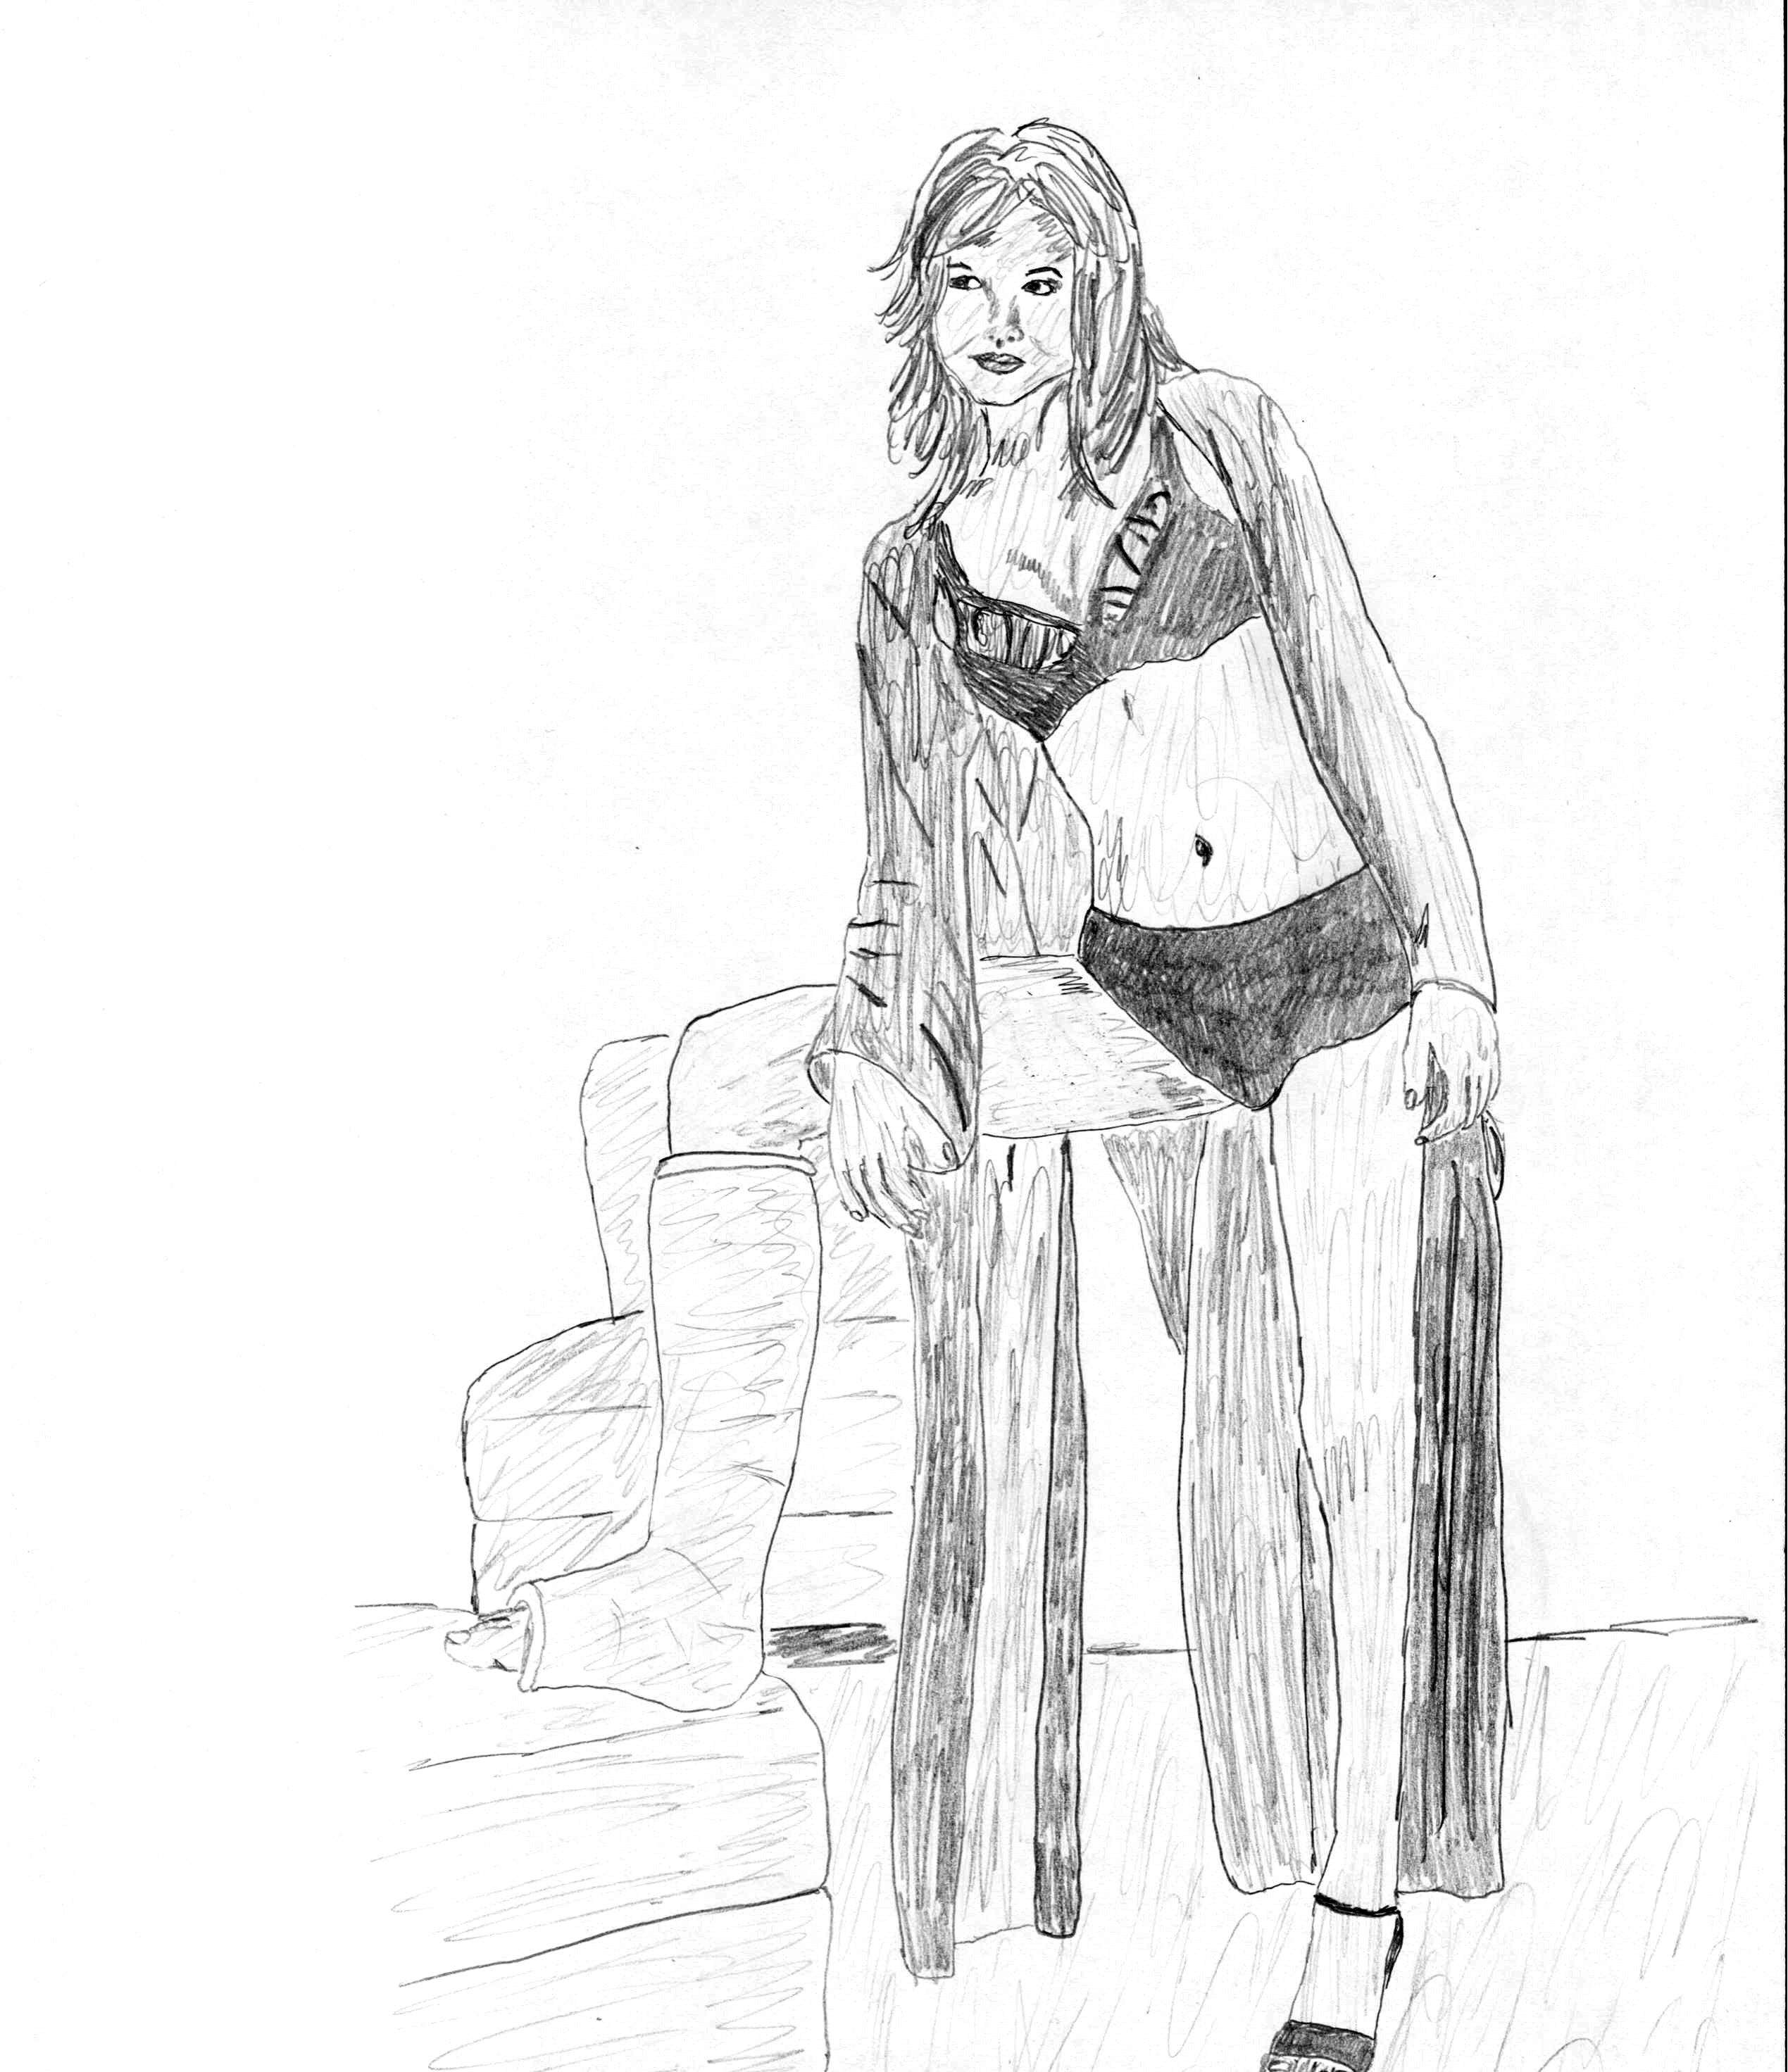
\includegraphics{images/kicks22.jpg}
\end{center}

\chapter{}

\chapter{}
Ah Mondays. Most people hate them, but I have come to love them. As the clock neared 9:00,
I was very eagerly awaiting Erin's arrival. It was cloudy outside, but it was going to be a
beautiful day inside.

When I heard the knock at the door, I knew the fun was about to begin. I opened the door,
and Erin looked great as usual. She didn't seem overdressed this time, yet was still dressed
very fashionably: She wore a black sleeveless jumpsuit. The zipper was unzipped far enough to
show a hint of cleavage, and the legs were short enough that it showed the top of the fantastic
pink long leg cast she had on her left leg. She had a Birkenstock on her right foot, and the bag
she carried was Gucci. She did like to do herself up.

I welcomed her inside, and we sat in the parlor and talked for a few minutes.

``I see you still have the long cast.''

``Yes,'' she said disgustedly. ``I go to the doctor on Friday. Hopefully I'll get a
shorter cast then.'' I thought to myself that I wouldn't be happy to see it go, though I DO want
her to heal.

``So, you're not scared off by today's plan?'' I asked.

``No. It's certainly going to be….. big.'' She said. ``But, then again, the money will be
really good, so I'm ready.''

Hmm- talking about the money. I think my internal alarm should have gone off, but all I
could think about was her situation: single, living alone, and unable to work. She was probably
just trying to keep the bills paid.

``Just remember that if this gets to be too much for you, just say the word, and we'll
stop and cut you out.'' I said. ``We should go ahead and get started- this will take some
time.''

She pulled herself up, and put her crutches under her arms. ``I'll be right there,'' she
said, heading for the bathroom.

I headed into the casting room, and started getting out the fiberglass rolls and padding.
I was going to need quite a bit today, and it was going to be great. I hoped it wouldn't be too
much for Erin. I reminded myself that it was she who had mentioned going to more and bigger
casts.

Erin crutched into the casting room, set her crutches against the wall, and hopped to the
table, where she turned and leaned back against the table, standing on her uncasted leg. She
unzipped the jumpsuit, pulled her arms out, and pulled it down. It was hard for me to not just
stop and watch her, but I had to remain professional. I did keep an eye on her out of the corner
of my eye. She hopped up on the table, and brought her right leg up and out of the suit. She
then stretched over to pull it off over the cast on her left leg. I wished I'd had a video of
this- a beautiful woman struggling with a cast to do an everyday activity. I couldn't help but
get a little heated up just watching it.

When she was done, she tossed the jumpsuit into the chair by the door, and sat up and
faced me. She looked great sitting there. She had a strapless bra and low cut underwear, just as
I had detailed to her on the phone.

``This bra is okay, isn't it?'' she asked.

``Yes, it's fine. We just needed for it to be strapless. Hang on, let me fill the bucket-
I'll be right back,'' I said.

I went through the usual routine of filling the bucket, and also retrieved the envelope
with the cash in it. My heart was racing at the thought of what was about to take place. I
calmed myself, and returned to the casting room. I handed her the envelope, and set the bucket
on the cart. She looked briefly in the envelope, and then lightly tossed it to the chair with
her clothes.

``Well, where do you want to start?' she asked.

``With the arm,'' I said.

She held out her left arm. I cut off a short length of one inch stockinette, and slit it
halfway up. I placed it over her thumb so that it extended past the end of her thumb, and the
flaps created by the slit lay on the front and back of her hand. Then, I took the three inch
stockinette, and cut off two and a half feet of it. I slid it over her arm to the elbow, and cut
a slit for her thumb to poke through. I took some two inch padding, and wrapped the thumb and
hand, making sure to use enough, but not too much of it. I wrapped the padding nearly to her
elbow, and ripped off the remainder of the roll.

After this was done, I looked up at Erin's face. She seemed to be watching what I was
doing, and lost in thought at the same time. I pulled on some gloves, and ripped open a roll of
two inch blue fiberglass, and dipped the roll until the bubbles stopped. I wrung it out, and
began wrapping her hand and thumb. I wrapped fairly quickly, but made sure to keep the
fiberglass smooth. I finished the roll by working it to past her wrist. I trimmed the length of
the stockinette and padding at the fingers and thumb, and folded it over. I then used another
roll of two inch fiber to anchor the ends down and give the cast the proper thickness.

After the second roll of two inch fiber ended at her wrist, I took a roll of three inch
fiberglass, and started wrapping it near her elbow. I worked down to the wrist and back. I had
enough thickness before the roll ran out. I held the roll in my left hand, and folded the
padding and stockinette over at the top of the cast, and then anchored it with the rest of the
roll. I did a little final smoothing of the cast, and then announced ``One down, one to go.''

She held up her casted left hand, looking at the cast curiously. ``This is a cast for a
broken thumb? She asked.

``Yes. That and certain types of wrist fractures.'' I said.

``It's getting warm.''

``Yes, it will be set soon. Keep your hand still for now, though. We probably should have
done that cast last, because we need to wait for it to set to do the other one.''

``Oops,'' she said.

``I need to get some things ready, so it will be okay,'' I answered.

I got the tall stool from the corner of the room and brought it to close to the table. I
then got my homemade leg stand, as well as two broom handles. I took Erin's left hand and
examined the cast. There were tiny droplets of water sweating out from the exothermic reaction
of the fiberglass drying. It still wasn't ready.

``Well, we still have a few minutes.'' I told her. ``Would you like something to drink
while we wait?''

``Sure, but not too much,'' she answered. ``I don't want to have to run to the bathroom in
the middle of this.''

I went to the kitchen and got sodas for us. As we sat and drank them, I tried to get her
to talk. I asked questions about her job, music, and what sort of activities she liked, but her
answers were fairly short and it seemed she wasn't too interested in talking about herself too
much. After we'd finished our drinks, the cast was dry enough to go on.

``I'll need you on the stool here for the next cast.'' I held out my hand, and she took it
with her right hand, and pulled herself up onto her right leg. She turned to line up with the
stool, and I held on as she lowered herself onto the stool. I picked up her casted left leg, and
slid the stand underneath it. Even though she was very distant, it was nice helping her move
into position.

I took the roll of twelve inch stockinette, and cut off a long length. I asked her to
raise her arms, and slid the soft material over her body after she'd done so. I smoothed it out,
making sure not to touch her in any way that might offend her. (I hoped) I pulled it down to
past her butt at the bottom, and left some of it bunched up at the top, which was in line with
her armpits. I wrapped six inch padding over the stockinette from the swell of her hips to her
armpits, and over her chest. I made sure to wrap the padding loose enough so as not to flatten
her breasts.

Before I opened the rolls of fiberglass, I warned her. ``As I make this cast, I'm going to
have to smooth it out, and that will include over your chest. I know we discussed this on the
phone, but you're sure you're okay with it?''

``Yes, it's okay.'' She said. ``I've been felt up before.''

``I'm not doing it to feel you up, Erin.'' I said. (Not entirely true) ``If you don't want
to, we can stop with what we've got.''

``No. Go ahead. I'm sorry if that sounded bitchy.'' She said.

``I just want to make sure you're okay with this.'' I replied.

``I'm fine. Go ahead.''

``Alright, ``I told her. ``I'm going to need for you to hold your arms up and out to your
sides. Hold on to these to keep them from getting tired.'' I handed her the broom handles, which
she took and positioned her arms.

I ripped open the first roll of five inch purple fiberglass, dipped it, and began wrapping
at her hips, working upwards. I deliberately started a bit low, but I would trim up this area
before the cast was finished. I worked my way upward, and I very much enjoyed the process. I
remained very professional, touching her only as much as was necessary to smooth the rolls as I
applied them. I continued wrapping her in the purple fiber until I had the cast nice and thick
from hips to armpits. I went ahead and pulled the padding and stockinette over at the top of the
cast, and anchored it. By the time I had finished this, the bottom of the cast was set enough to
trim. I took my cast saw, and cut the lower area of the cast back enough to allow her to move
her hips, but left it low in the back, and in the center of the front. I pulled the padding and
stockinette back, and anchored them with a final roll of fiberglass.

We waited a few minutes while this dried. Now, she was asking me questions. Mostly about
the cast fetish, and the man who was financing this. I answered her questions as best I could,
keeping up the facade of there actually being an external financier. She seemed to be very
interested in the type of person who would pay for what we were doing. I fended off most of the
questions with the ``I'm just doing my job'' dodge. I was starting to wonder if she might be
angling. I hoped I was wrong. I had been waiting for her to soften up a little bit. I was hoping
she'd get friendly enough for me to ask her out, but now I wondered if I wanted to. I reminded
myself that for the time being, I just need to enjoy the day.

After the body cast had dried, I helped her into the wheelchair, and pushed her into the
living room, where I took pictures of her in various poses: in the wheelchair, standing on
crutches, sitting and lying on the couch. I decided to take her to the breakfast nook, and we
took several more pictures in various poses. One pose, where she stood by the window, leaning
against the wall without the crutches, was the one that I sketched her in. Today had been a step
forward in that I was able to get her to smile more, but even the smiles seemed forced and
insincere. Still, she was beautiful, and she really filled out a cast nicely. I suppose I needed
to stop thinking of her in terms of a romantic possibility, and just as an employee.

After the sketch was done, I wheeled her back to the casting room, and cut her out of the
casts. Despite the body cast being big, it was fairly quick to get her out, as it only required
a straight cut up each side. I cut the stockinette and padding on only the left side, and freed
her from the cast. Five minutes after that, the thumb spica was off, also. I handed her a cloth
to wipe the dust off of herself.

After she'd done this, she grabbed her jumpsuit, and got herself dressed. We said our
goodbyes, and she crutched down the sidewalk. I wasn't sure what to think of her, now. I'd been
highly attracted to her, but now I wasn't sure. Maybe I'm wrong. Either way, I'll have to wait
until next Monday to find out any more.

After I had cleaned up from the casting session with Erin, I knew I had to get out of the
house for a while. The clouds of this morning had given way to a beautiful day, so I got out the
Harley and went for a ride.

I rode through the town, enjoying the feel of the afternoon sun and the wind in my face.
Before I knew it, I was out near the local mall. I had wanted to get a new CD from one of my
favorite artists, so I went to the Borders store located across the street from the mall.

I went straight to the music section, and found the disc I wanted. I was browsing some of
the other music when something caught my eye. Over in the section near the magazines and the
overpriced coffee counter, there was a woman sitting at a table reading. She was seated with her
back was to me, but she had very pretty long brown hair, and appeared to have a nice figure from
what I could see. What had caught my eye was the pair of aluminum crutches leaning against the
table.

Being a caster, I had to move in to get a closer look at this person. Not wanting to be
obvious, I went to the magazine section and picked up a copy of Hemmings Motor news. I went to
the coffee counter and ordered a double espresso. I turned from the counter and walked toward
the table next to the woman.

As I got closer to the table, I almost dropped my coffee. I noticed that she had her left
foot up on a chair. Her ankle was wrapped in an Ace bandage. She was wearing shorts and a
t-shirt, and she was indeed very beautiful. It was Monique!

I walked toward Monique, and as I neared, she looked up. When she saw me, her face turned
red.

``Hi, Quinn.''

``Hi, Monique, what happened?''

She paused for about a half a second, and said ``I tripped on the steps at my apartment.
Nothing serious, just sprained my ankle a little bit.''

``Ouch!'' I said. ``Did you see a doctor for it?''

``Yes. They even X-rayed it. I wondered for a while if I might get a cast for more than a
few hours. As it tuned out, it's just a mild sprain. They wrapped it, and gave me the crutches.
Told me to take ibuprofen and stay off of it for a few days.''

I smiled jokingly. ``If you want a cast for more than a few hours, there's a less painful
way to do it.''

She blushed a little again, and then said ``Where are my manners? Sit down.''

I took the chair opposite of her, and sat down. ``Do you need to skip this Friday?'' I
asked, sipping the strong coffee.

``No, no- I'll be there,'' she said. ``It's really not very bad. I can walk on it already,
but it hurts a lot if I walk too much on it. But it's not anything to keep me from working. Do
we have our…assignment yet?''

I had to think fast. ``Well,'' I started, ``he wanted to see you outdoors in a city
setting. I was thinking about Cincinnati. He said he liked you in leg casts, so he mentioned a
below the knee cast on one leg, and an above the knee cast on the other.''

``I can do that just fine.'' She said. ``I've been getting some practice with the
crutches, too.''

Despite the fact that I really felt some anonymity towards Monique, I didn't want to
aggravate her injury. ``We can bring along the wheelchair, just in case it gets to be too
much,'' I told her.

``That's fine, but I should be alright.''

I got up from the table. ``So, I'll see you Friday at 9:00?''

``I'll be there. She said.
I went to the cash register, paid for my disc and the unread Hemmings. Then I got on the bike
and headed back home, thinking about what I had just seen. It seemed somehow surreal.

\begin{thought}
After Quinn had gone, Monique could not concentrate on her magazine. ``Two leg casts, and
in public, too!'' She thought to herself. ``I can't wait! There will be a LOT of people around.
It's going to be a blast. She got up, dropped her empty cup into the trash, paid for her
magazine, and crutched out to her car. As she drove home, she replayed the meeting in the store
in her mind. It was very nice to see Quinn, and she'd enjoyed their chat, even if it was brief.
She wished she could've gotten him to stay and talk longer, and maybe about something besides
business, even if business to him was pleasure to her. She'd really been caught off guard,
though. The way she was feeling about Quinn played a part in her feeling off guard, but she was
also sure that he would see right through the huge lie she'd told him. She was afraid he would
know that she'd never hurt her ankle, but was faking it with a bandage and crutches she'd gotten
at the drugstore last Friday.
\end{thought}

\newpage
\begin{center}
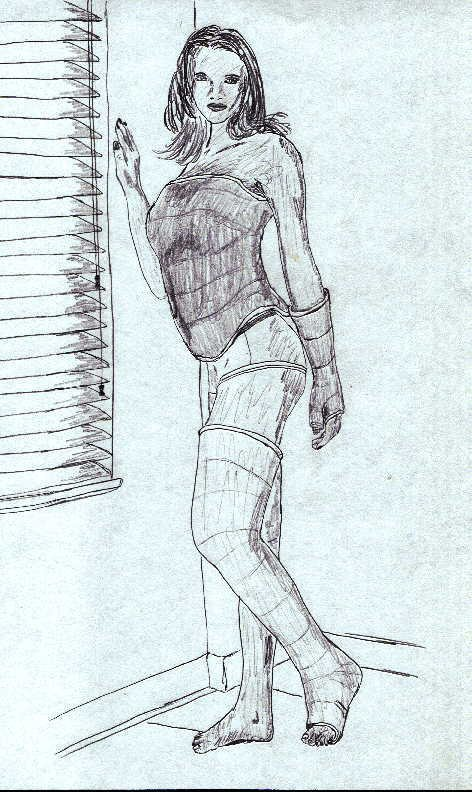
\includegraphics{images/kicks24.jpg}
\end{center}

\chapter{}

\chapter{}

\chapter{}

\chapter{}

\chapter{~}
I watched the Sunday evening sun set with my new house guest. We were sitting on the deck,
holding hands. The setting was very peaceful despite the ugly stump where the beautiful Oak had
stood, and the crushed pickup sitting in front of the garage. We sat in silence, and I was
pleasantly surprised to find the silence was in no way awkward. It was good just to be with her.

We'd been through an intense weekend, to say the least. I'm sure we were both a bit
emotionally exhausted, yet I found myself content, just sitting with her, hand in hand.

Monique broke the silence.

``Quinn, let's go to Cedar Point. I'll treat.''

For those of you who may not know, Cedar Point is an amusement park in northern Ohio. It is
one of the oldest amusement parks in the United States, and is renowned for its great roller
coasters.

``Are you serious?''

``I'm serious as a heart attack.'' She said with a smile. ``I've got some extra cash, thanks to
this weekend, and I have someone to share it with, also thanks to this weekend. We could leave
tomorrow.''

I was taken aback, yet the idea was appealing. It had been a while since I'd done any roller
coaster riding, and Cedar Point is rated the best park in the world for coasters. As my mind was
starting to like the idea, I thought of Erin, who would be here at 9:00 tomorrow morning, and
Samantha coming Wednesday.

``Monique, I have a model coming tomorrow morning.''

Her face fell a bit at this, then she said ``We could leave after you finish.''

I was about to tell her about Samantha, and how one day wasn't enough time to fully
experience the park, when the side gate opened, and my landlord walked in.

``Hello, Mr. Moore,'' I said.

``Hello, Harlan. I was just wondering if the power had been restored, here. I tried calling,
but couldn't get through.''

``The power is back,'' I replied. ``But it sounds like the phone is still out. To be honest, I
hadn't checked.''

He went on. ``I also wanted to let you know that the insurance adjuster will be out to check
out the house tomorrow. He'll need to get inside. Will you be home?''

I hadn't considered it, but if there was going to be someone in the house, I would rather
not have to explain why I was putting casts on a perfectly healthy woman. Thinking quickly, I
said ``I'll be here some, but not all day.''

``OK,'' Mr. Moore said, but I'll need to give him a key so he can get in.''

``That's fine,'' I replied.

``Hopefully, I'll have the repairmen out Tuesday to start work. Wednesday at the latest,'' He
said.

Hmm- Insurance adjusters and repairmen. My little casting studio was starting to look like
it wasn't going to be very suitable for casting this week. On the spur of the moment, I said
``actually, Mr. Moore, I'm thinking of taking off for a few days on a trip.''

``That might not be a bad idea. Just make sure not to leave anything valuable lying around.''

``I won't.''

With that, he said goodbye and left. I turned to Monique, who was looking at me with a
playful smile. ``It sounds like someone may have reconsidered,'' she said.

``Well, I won't be able to work in a construction zone. And it's not everyday that a
beautiful woman asks me to go ride roller coasters.''

``A beautiful woman asked you to go ride coasters with her?'' Monique said indignantly. ``Who
is she? I'll kick her ass!''

I shook my head, smiled, and kissed her.

``And besides,'' she added. ``Just because we're going away for a few days, it doesn't mean you
can't work.'' She lifted her eyebrows at this last comment.

Monday morning, I woke up, showered and went downstairs to wake Monique. I really wanted to
have her in my bed with me, but I knew it wasn't time for that, at least not yet.

Erin wasn't coming today. I'd used the cell phone to call her last night. She wouldn't have
been able to make it anyway. She'd been at her doctor's office when the storm hit. She had told
me that they were going to take off her cast, and replace it with a shorter cast she could walk
on. The power went out when they were cutting the cast, and they'd had to tape it back up and
told her to come back today. I also had called Samantha. I got an answering service, and left
her a message that we wouldn't be able to work this week due to repairs of the storm damage.

After Monique had showered and dressed, she informed me that she needed to go do a bit of
shopping before we left.

``OK. We can get some breakfast, and then go shopping. We can't leave until the truck gets
towed away.''

I got the bike out of the garage, and we rode off through the devastated town. Cleanup was
still going on en masse. We found a restaurant open, and stopped for breakfast.

While we were eating, she kept talking about the trip. She clearly was excited about it.

``This is going to be a fun trip. I know I mentioned doing some casting while we're there,
but if it's too much like work for you, I'll be very content just to be with you.''

``Monique, what made you think that casting was like work to me? Granted, it is my job, but
when did I ever say I didn't enjoy it?''

\begin{thought}
OK, now I know I'm dreaming, Monique thought to herself. He'd never really said so until
now, but she had secretly hoped that Quinn enjoyed this as much as she did. Saturday night, when
she'd opened up to him about her feelings, she was so happy to learn that he was attracted to
her that she'd not asked about his feelings about casting. She'd been afraid of what she might
hear.
\end{thought}

``So, you enjoy this weird 'hobby' too?''

``Yes, very much,'' I replied. ``It was no accident that I hooked up with this job.''

``I think I'm in heaven,'' she said, as she pulled me into a kiss.

``So, let's go shopping, and get on the road,'' I announced.

Not expecting to find many stores open locally, we headed out of town and across the state
line into Ohio. We went to the Cincinnati area, and found a mall that was opening for the day.
She bought some clothes and a pair of sandals. While she was in one of the stores, I waited
outside under the premise that I was going to call the boss about our plans. I hated lying to
her, but she'd said that she didn't like rich people, and I could not shake that thought. To be
honest, that thought was starting to scare me- a lot.

When she returned, I told her that we'd been given the green light to get any supplies we
might need, and to cast as much as we wanted while on the trip. She was very pleased to hear
this.

Shortly after noon, we arrived back at the house. The phone company was there, and the
repairman informed me that he was just finishing up and the phone should be working. The cable
television repairman was just arriving to put those lines back up. I parked the bike, and
Monique and I went inside to pack some clothes for the trip. I also packed supplies and tools
from the casting room. As Monique was helping me load the materials in the Mustang, she asked
``Is there enough left to make me a traveling cast?''

``You haven't been out of the body cast much more than 24 hours.'' I said. ``You already want
to be in another cast?''

``Sure- why not?''

I was wondering now if I was the one in heaven. She really DID like wearing casts. My
little voice be damned, she was pulling me in.

``Alright. How about a nice leg cast for the road?''

She liked the idea, so I instructed her to take off her shorts and shoes while I retrieved
a few things from the car. When I returned, she was sitting on the casting table in her tank top
and underwear. I slid stockinette up to her left thigh, and then wrapped it from the top down in
padding. I filled my bucket with water, and then began tearing open the packages of pink
fiberglass. I wrapped her leg from slightly higher than mid-thigh downward, putting enough of a
bend in the knee to make sure she'd be comfortable sitting in the car on the drive.

\begin{thought}
Monique felt almost in another world as Quinn wrapped her leg in pink fiberglass. It was a
delightful array of sensations for her. Watching the man she was falling in love with wrapping
the pink tape, the fruity smell, the feeling of gentle pressure as his hands encased her leg in
rapidly setting fiberglass. She wasn't sure where things would lead between them, though she
knew where she wanted them to lead. She decided to just enjoy the moment, and the moment was
truly wonderful.
\end{thought}

I packed the items we'd used in the car while Monique remained in the cast room, waiting
for her cast to dry. I got the aluminum crutches for her. She hoisted herself up from the table,
and hobbled around the room.

``OK, I'm ready to go!''

``We just have to wait for the tow truck to get here. As soon as they haul the truck off, we
can get going.''

We passed the next hour just talking about our trip. We were both pretty excited about
going, and it showed. She wanted to check something online, but we had to wait until the cable
technician was done, since I have a cable modem for internet connection. When service was
restored, she went to the Cedar point website, and was surfing through pages rapidly until she
found what she was looking for, and called me over.''

``Quinn, come look at this!''

She was reading from a page with tips for guests with disabilities. She showed me that
certain guests can get a special access pass that allows them front of line access. She then
went to another page that showed that they would let guests with casts ride if their casts did
not cover the knee or elbow. She then looked at me slyly.

``Are you thinking what I'm thinking?'' She asked.

``I'm thinking you want to go to the park in a cast, just so we don't have to wait in
lines.''

``No, I want to go to the park in a cast for the fun of it,'' She answered. ``I'm just
thinking that the front of the line pass seals the deal.''

``I'm thinking that you're incorrigible.'' I said.

She laughed at that, and the laughter was interrupted by a knock at the door. I went to
answer it, and it was the towing service. I took him out back and showed him the truck. He made
a comment about how bad the truck was damaged (as though I couldn't see for myself) and went to
back his truck up to it. I left him to his work and went back inside.

We closed up the house, and when the truck was hauled off, we headed out. We stopped for
lunch, and Monique got some long looks from guys at the restaurant. She was quite a sight, a
stunning brunette, seeming to be having a lot of fun in spite of a broken leg.

We had a great trip north, alternating between talking and just listening to music. We
weren't in a terrible hurry to get there- we planned on taking the whole afternoon. We made
several stops to stretch our legs. Well, I stretched my legs, and she stretched one of hers. On
one of the stops, I decided to do a sketch of her with the car. She stood in front of the car on
her crutches while I drew. When I was done, I showed her my work, which she approved of. We then
continued north.

We arrived at the park at about 4:00 p.m. local time. We headed around to the hotel inside
the park, and checked in. Our room had a great view of Lake Erie. When I had carried in our
luggage, including the supplies, we went out on the balcony overlooking the lake and watched the
sailboats out n the lake by the lighthouse. Monique broke the silence.

``So, what shall we get up to tonight?''

``Why not go and hit a few rides before the park closes?'' I asked.

She liked the idea, but couldn't ride in a long leg cast. I assumed the rooms around us
were probably empty, and using the cast saw wouldn't disturb anyone. I used the cast saw to cut
away the portion of her cast over the knee, and then pulled back some stockinette and padding. I
wet a roll of pink fiberglass, and anchored it down, then wrapped down to her foot to add some
strength to the cast.

We sat and watched the boats awhile while the cast dried, then I strapped a cast shoe on her
foot, and we headed out to the park.

\newpage
\begin{center}
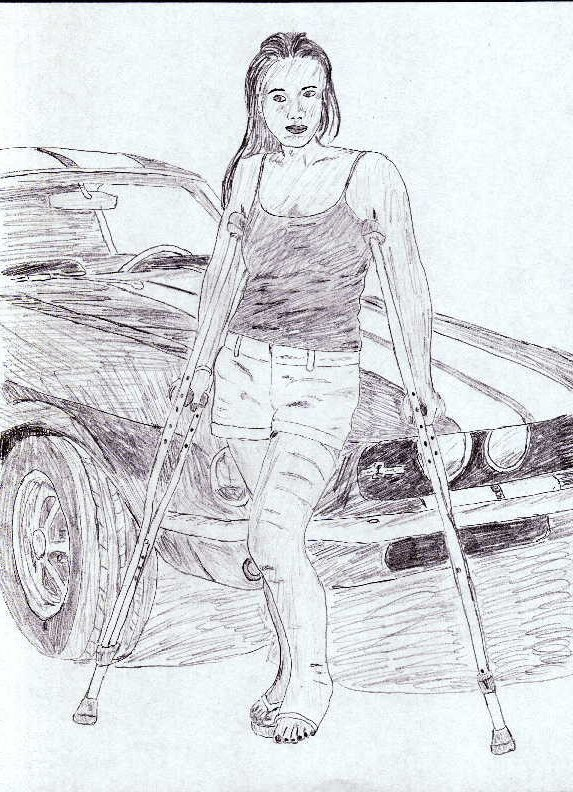
\includegraphics{images/kicks29.jpg}
\end{center}

\chapter{}
We left the hotel and headed to the park. Despite the limp caused by her cast, Monique's
pace was very quick. We made our way to park operations, where we rented a wheelchair, and
received our paperwork for special access. Her pass allowed us to bypass the lines completely
for most rides. For the most popular rides, we were given a time to come back, and when we
returned, we were able to get right on.

She got a lot of looks from people in the park. I noticed several of the guys doing double
takes at her, and found myself wondering if they were looking at her because of her cast, of
simply because she was so beautiful.

Riding the roller coasters was great. The coasters there are among the very best in the
world. Her cast presented a few minor problems for us getting into and out of the cars. On a few
of the coasters, the foot space was so limited that she had problems getting the cast into a
comfortable position. The most interesting event on a ride was on the Raptor, a coaster where
the track is above the car and your feet dangle below. On that ride, the attendants asked that
she sit in the seat on the far left. I assume that was so that her cast wouldn't swing around
and hit someone.

\begin{thought}
Monique was having the time of her life. Being pushed around in the wheelchair was great.
She felt very pampered by Quinn, who seemed to be having a lot of fun, too. The wheelchair also
drew a lot of attention, and she had to admit to herself that she enjoyed the attention. She
found herself wondering if any of the men she noticed looking at her two, three, or more times
was in fact, a closet caster. The coasters were awesome, the park was beautiful, and the smell
of the lake was scintillating. As the night wore on, and the park neared closing for the day,
she knew there was one thing left that they had to do.
\end{thought}

``Quinn, let's go turn the wheelchair in, and go for a walk on the beach.''

The idea seemed great to me. It wasn't the ocean, but Lake Erie is big enough to feel like
it. The evening was beautiful, Monique was beautiful, and the beach was the perfect place to
wind up our evening out.

``That's a great idea, let's do it.''

I wheeled her back to guest relations, we turned in the wheelchair, and we headed for the
beach. It was a fair distance, and though she kept up a quick pace as she limped along, I found
myself concerned for Monique's casted foot. I didn't want her to end up with a blister.

``How's the foot doing?'' I asked. ``It isn't hurting, is it?''

``No, it's fine,'' she said. ``The cast shoe is pretty soft- it feels as soft as wearing a
sneaker.''

``Okay- just checking.''

\begin{thought}
``He thinks of everything,'' she thought to herself. The level of thoughtfulness that Quinn
showed to her was one of the things she found herself coming to love about him. She was also
discovering that his unselfish concern for her was making her open herself more to him. She
thought back to only a couple of months ago, when she was very emotionally withdrawn. She hadn't
been a cold, unfeeling person then, she just kept a very solid wall between her heart and the
world. That was then. She had first noticed that she was unable to stop Quinn from reaching her,
and then she noticed that she didn't want to keep him from it. As they reached the beach, and
walked out onto the sand, the moment became one she didn't want to end.
\end{thought}

Walking along the beach with Monique was great. We walked half the length of the beach
without even speaking. That was something about Monique that I had never experienced with anyone
before- long silences were not uncomfortable. Neither of us felt the need to entertain or be
entertained, just being together was enough. We walked past the beach chairs, most of them
empty, a few occupied by sunburned parents as their children ran along and stomped the remains
of the days sand castles. It was Monique who finally broke the silence:

``Oooh, I wasn't expecting THAT.''

``What?''

``Sand in the cast.''

``Ouch,'' I replied. ``We should have thought of that. Is it really uncomfortable?''

``No,'' she answered. ``It's not too bad. I don't want to walk forever like this, but I
wouldn't trade this walk for anything.''

``We'll get you out of that cast as soon as we get back to the room,'' I said, then added ``I
wouldn't trade it, either.''

She smiled, and gave me a quick kiss. We continued walking along the beach until we got
close to the lighthouse. We stopped and watched the light blinking out over the lake for a
while. As we stood there with arms around each other, I was lost in the sensations. The rhythmic
blinking of the light, reflected on the calm surface of the lake; the smell of the water, mostly
pleasant; the sound of the waves licking at the sand; the coolness of the night air, offset by
Monique's warmth pressed hard against my left side.

I honestly could not tell you how long we stood there. It may have been a few minutes, or it
may have been a half hour. Time wasn't too important at that point, and I didn't bother to
check.

It was again Monique who turned to me and broke the silence.

``Quinn, let's head back to the hotel,'' she said.

``Okay, let's get you out of that cast.''

``And into another one?'' she asked with a smile.

``If you like, absolutely,'' I answered.

``Or two, or three?'' she added with an impish smile.

I laughed at her. ``You're incorrigible,'' I told her.

``Count on it!''

After we'd made our way back to the hotel, we went into the bathroom, and cut the cast from
her leg. We did it over the bathtub, so a quick splash of water from the faucet took care of the
cleanup. We decided to leave her uncasted until after we'd eaten dinner, which we ordered from
room service.

Over dinner we recalled the day, and the fun we'd had. We talked of the coasters we'd
ridden, and what we wanted to ride tomorrow. We were truly having a great time together. As the
conversation unfolded, I began to realize that this was a fantastic trip in every regard. I also
realized that the fact that she'd spent most of the time in a cast was not the high point of the
trip. It was wonderful, without a doubt; but the trip and the company would have been wonderful
without any ``hardware.''

As we finished dinner, we stayed seated at the table, talking. Monique brought up the
subject. ``So, when do I get my new cast?''

``Anytime you'd like. If you want it tonight, we can do it whenever. If you'd like a free
evening, we can wait until tomorrow morning. Or skip it entirely.''

``Skip it entirely? Perish the thought!'' she answered playfully. ``What kind of cast model
would I be if I wimped out on you, now?''

I shook my head. ``Monique, I think you're slightly more than a model, now.'' I looked her in
the eye. ``At least I'm hoping you are. I'm having a great time with you. We can pack up the
supplies and just hang out together. I would have the time of my life with you whether or not we
cast you.''

I wish I could have described the warmth in the smile that she broke into at my comment.
She didn't answer my statement immediately. She got up, and walked around the table to my side.
She turned me to face her. She then climbed onto my lap, facing me, with her legs wrapped around
me.

``I'm very glad to hear that, I really am. I'm having the time of my life with you, too, and
I enjoy wearing the casts, for several reasons. I'd hate it if the only reason you wanted to be
with me was for the way I fill up a cast.''

``Monique,'' I replied, ``it isn't.''

She smiled again. ``And I know that.'' We melted into a long, passionate kiss that lasted…
well; I really couldn't tell you for sure how long it lasted. It might have been a minute, it
might have been ten minutes. Hell, it might have been more- time wasn't the issue at that
moment.

After the kiss, we just sat there, gazing at each other for a few moments. Monique spoke
first. ``But, any woman who doesn't like to dress to please her man doesn't deserve him, now
does
she?'' She asked with the familiar, playful smile.

I couldn't help but smile back. ``Well, it's nice, but I hardly think it's the key element in
a good relationship.''

She rolled her eyes and shook her head in mock disgust.'' So, am I going to have to cast
myself, now that you're all serious?''

``No, ma'am, I'll be happy to oblige your needy leg. Is your ankle hurting much?''

``It hurts quite a bit, but it's not near as bad as my arms.'' She said, dangling both arms
like dead weight.

``Arms?'' I asked with eyebrow lifted.

``Yes, they're in agony. It's like they are on fire- my shoulders, too. ''

I was stunned, and it must have showed on my face.

``What's the matter?'' she asked. ``I know from firsthand experience that you can make a nice
shoulder spica. What's so hard about adding in the other arm?''

``Nothing, really. I'm up for it if you're sure you are.''

``Eh, I've worn bigger,'' she retorted nonchalantly.

I smiled at her. ``Anything the lady wishes will be my happiest duty.'' And started opening
up the supplies. Fortunately, I really HAD packed us heavy on goodies. While a double shoulder
spica would seriously dent the mini-stash we had, it wouldn't exsanguinate the supply.

She brought her chair over to where I was, and sat in front of me, holding her left leg out
toward me. ``The leg first doctor, if you please.''

``Let's head to the bathroom,'' I said, pulling on a pair of gloves.

\begin{thought}
Monique watched as Quinn smiled, and began to cast her leg. Though having him wrap padding
and fiberglass on her was nothing new, she still enjoyed it more each time he did it. The leg
cast was nothing major, just a well padded short leg cast for tomorrow's venture into the park.
He worked quickly, but skillfully. After a few minutes, he was pulling off his gloves and they
both admired his work. It felt good, it looked good, and she was seriously anticipating what
came next. They shared a smoke, and as soon as they were finished, he gloved back up, and
slipped her tank top off. She found herself secretly hoping he would take off her bra as well,
but he did not, and she knew why- the bra would help keep her breasts from flattening under the
cast as it was applied. He cut a section of the large stockinette and slid it over her down to
her hips. He then pulled it up to her armpits, and then slit it on each side so he could pull it
up in the front and back, securing it to itself over each shoulder. He then cut two long
sections of the smaller stockinette and pulled them up first the left arm, then the right.

He started wrapping padding on the left arm, and wrapped it from her hand to her upper arm.
He then repeated the process on the right. He got some wider padding, and wrapped from just
below her waist upward, covering her to her armpits. Then, back to her arms, wrapping the top of
each arm, and shoulder. Monique looked away from Quinn's working on her. There was a full length
mirror on the bathroom door, and she watched him work through the reflection as her upper body
became soft-looking and snowy white.

After the padding was done, Quinn put on his gloves and ripped open a roll of pink
fiberglass. He began wrapping her left hand, and worked his way up her arm. After the first roll
was finished, he went back and anchored the padding and stockinette at the hand, and then
proceeded up the arm. A few rolls later, he was wrapping the shoulder and around her chest. With
the left arm finished, he repeated the process on the right arm. It was a bit tiring, holding
her arms out at her sides, but it did not detract from the exhilaration that she felt at the
cast application. As always, getting the cast applied was a sensory treat: the smell of the
fiberglass; the gentle sound of the wet fiberglass as he pulled it from the roll as he wrapped;
the vision in the mirror of him working as her body became more and more encased in the setting
pink shell. Most of all, she enjoyed the sensation of gentle and slight pressure as he wrapped
and molded the material on her body.

When he had finished the cast by anchoring it at her waist, he pulled off the gloves and
stepped back to admire his work. The satisfied smile on his face told Monique that Quinn liked
what he saw.
\end{thought}

Monique looked unbelievable in her casts. The short leg cast was molded very well. It did
not hide the beautiful shape of her leg, but merely accentuated it. The double shoulder spica
was fantastic, if I did say so myself.

We waited a few minutes while the cast dried. I went and retrieved the cast shoe, and put
it on her casted left foot. I helped her to stand, and then steadied her as she walked into the
bedroom. I helped her into bed, and went to get my sketchpad. I was starting to feel a bit
tired, but I couldn't wait to draw her like this.

\begin{thought}
As she sat on the bed, watching Quinn work over his paper, Monique was enjoying the feel of
the huge cast. She found she could twist a slight bit inside the cast, but not much. She was
truly held fast from her waist to her neck, and it was wonderful. She was totally helpless and
dependent on this man she was falling in love with, and it was a wonderful feeling. She was
surprised to be able to admit to herself that she was falling in love, but the self-realization
felt good. The fact that she found herself able to trust him when she was so unable to help
herself warmed her from the inside. Although they couldn't do it now, she wondered what it would
be like to be out in public in a cast this massive. It seemed that everyone noticed her when she
was wearing just the short leg cast. What would it be like if she was out like this? She just
might have to bring it up to Quinn sometime. It was one of the things that they could do down
the road. She hoped that road was a long one.
\end{thought}

When I was done with the sketch, I glanced at my watch and couldn't believe how late it had
gotten. No wonder I felt tired. I noticed Monique had a sleepy look in her eyes as well, so I
helped her into bed, and then got in myself. I kissed her goodnight, and cuddled into embrace
her as best I could. I found that if I lay a pillow on her upper arm, I could rest my head on
that. I slipped one arm underneath the pillow she had her head on, and laid the other arm across
her casted midsection. It wasn't long before I was asleep.

\newpage
\begin{center}
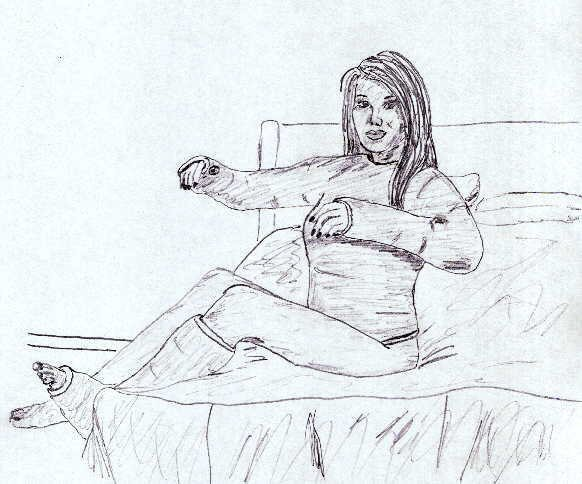
\includegraphics{images/kicks30.jpg}
\end{center}

\chapter{}

\chapter{}
As I piloted the Shelby south on I-75, the events of the last 5 days replayed in my mind:
The storm, the park, and Monique. A lot of Monique.

Every once in a while, I'd look over at her, she had fallen asleep about an hour into the
trip home, and was still leaned against the door. I couldn't hear her soft snoring over the
rumble of the big engine, but I knew the sound. Yes, I knew it well.

Last night had been unexpected, but it had been fantastic. She was very loving and
passionate. I have never been with a woman who seemed to put as much of herself into lovemaking
before. It truly had been beautiful. Waking up next to her was great, too. Watching and
listening to her sleep until she woke up, and watching her walk to the bathroom naked except for
the pink cast on her left leg.

We were headed home, and there was a lot to deal with once there. There was the issue of
the damaged house- the repairmen would hopefully be started by now. I also had to get some new
transportation, since the only vehicles I had left were an antique muscle car and a motorcycle.
And then, there were two other women to think about. Two women who were expecting to come and
earn money next week. I wondered how Monique would feel about them. Honestly, I didn't really
care if I casted them or not. They were both very attractive, and casting them had been
enjoyable, but with the relationship developing with Monique, (wow, that was something I
wouldn't have expected to say a week ago!) casting Erin or Samantha wasn't as appealing as it
used to be. Yet, I just wouldn't feel right cutting them off with no warning, not when we had
standing appointments.

\begin{thought}
Monique was dreaming. In her dream, she and Quinn were in Paris, walking along the avenue
in the old town where her father used to do his portraits. In the dream, it was warm, and a
light breeze was blowing. Quinn wore his usual T-shirt and jeans, she wore white linen
drawstring pants and a light blue shell top. She was showing him the areas she frequented when
she lived there. As she told him of her memories at each stop, she was speaking French, and he
was answering in French. She felt very contented, walking hand in hand with Quinn in the
afternoon sun, sharing her early life with him. She awoke to find that they had stopped at a gas
station. Quinn was setting the parking brake, and opening the door.
\end{thought}

``I'm sorry I dozed off on you,'' she said. ``Where are we?''

``That's OK, you're good company even when you're asleep. We're almost to Cincinnati.''

``Wow, that's a long way'', she said, as she got out of the car, stood up, and stretched.

She excused herself, and headed toward the restroom. I watched her walk away, with her
slight limp from the cast on her left leg. She'd wanted to keep it until we got home, and I was
happy to oblige, though she'd had her left leg in one cast or another for most of the last five
days. We couldn't keep her casted all the time, as there was muscle atrophy and other medical
complications that were possible. I met up with her inside, and slipped my arm around her waist
as we went to the register to pay.

The rest of the trip home, she stayed awake, and we talked. We talked about a lot of
things. We had a lot to share with one another, and we just took turns talking about our lives
before we'd met. One of us would say something that sparked a memory in the other one, and a new
area of the conversation would open.

We arrived home shortly after 6:00pm. The storm that had changed our lives so dramatically
had affected the town equally as strong, but where it had been positive for us, it had been
negative for the town: once large trees were now cut back to nothing but trunks, their fallen
branches cut up on the ground beside them. Many houses had their roofs covered with tarpaulins,
and far too many houses had serious damage, or were nothing more than piles of rubble.

As I neared the house, I could see that my (our?) roof was entirely covered with a tarp. As
I turned the corner, I saw a dumpster in the driveway, but there was enough room to get into the
garage. We parked, and a quick peek into the dumpster told me that the repairs were under way-
the dumpster was full of old shingles and guttering.

That evening, I brought up the issue of Erin and Samantha. I really wasn't sure how she'd
take it, but her response had not been all that surprising.

``Quinn, you had an agreement with those women before 'we' happened. If you broke the
agreement with no warning, I'd think less of you.''

I just shook my head and smiled at her. ``You know you're amazing, don't you?''

She cocked her head, raised her eyebrows and said sarcastically ``Yes, but keep telling me,
I like to hear it.'' Then she broke into a smile. Then she took a more serious tone.

``I feel totally at ease with you. I've never trusted anyone much, but with you, it's just
natural. Besides, I know how professional you are.''

At that point, I had an idea.

``Monique, if you'd like, you can help me out with the casting sessions.''

She thought about that a bit. ``That might be fun,'' she said. ``I might have a little cast
envy, but it might still be fun.''

``Speaking of casts, we probably ought to get you out of that one,'' I said, pointing to her
left foot.

She didn't seem thrilled about getting rid of the cast, but we headed for the casting room,
and I cut it off. She walked around a bit to work out some of the stiffness.

Thursday, we went vehicle shopping. We'd left a lot of things undone when we'd taken off
for Ohio and she'd discovered that the shop where her car had been was leveled, and her Firebird
had been destroyed. We were both without everyday transportation. She had planned to take some
of the money from the weekend of the storm and find something used, but I had a different idea.
I needed a pickup truck, but it wasn't always the best vehicle for publicking. We decided that
in addition to a pickup truck, I'd also get a SUV, which would serve well for public cast
adventures, and she could use it to get back and forth to work and school, once it started
again.

When we got home from the dealership, I saw the roofers there, and after talking to them a
bit, they assured me they would be done by Friday afternoon, or Saturday if it rained. Thursday
night, I called Erin and Samantha. I spoke to Erin, and she told me she'd gotten her new cast on
Monday. She said the doctor told her she was healing well, but that she still couldn't go to a
cast below the knee. The good news, she informed me was that they'd given her a cast with her
knee straighter, and it had a walking heel, so she was finally walking without crutches, and was
happy to be rid of them.

When I called Samantha, I got her voice mail, so I left a message stating that I would be
ready the following Wednesday, and asking her to return the call to confirm.

I realized that my stock of supplies was dwindling. I'd used a lot of fiberglass in the
last week- I'd made Erin's body cast and thumb spica, Monique's huge hip and shoulder spica, a
couple of leg casts, and a double shoulder spica. I decided to make a run Friday to get some
more fiberglass and padding. Considering where things were at with Monique, and her preferences,
I also planned to get a good bit of plaster, too.

I invited Monique along, but she was scheduled to work during the day. We'd had a
discussion about her working. She really didn't have to work, but she insisted on paying for her
schooling. She also said that she'd send some of the money to her mother to help out. Of course,
money was nothing to me, but she didn't want me to pay her way for everything. I couldn't talk
her out of it, so I settled for providing living expenses.

\begin{thought}
Friday, after work, Monique returned home, grabbed a quick shower, and put on shorts and a
T- shirt. She really didn't know when to expect Quinn, but she tidied up around the house a bit
while waiting for him. In the front room, she saw the radio they'd used Friday during the storm.
Seeing it reminded her of how intense the day had been, She'd been truly frightened by the
storm, but at the same time, she'd been thrilled to be with Quinn, and to be in such a huge
cast. She put the radio back into the closet she'd seen him get the radio from, and she had a
strange thought- there had been a flashlight there, and they'd taken it downstairs when they'd
gone for shelter from the storm. She was pretty sure they'd left it there, and went to go get
it.

She flipped the light switch, and headed downstairs, remembering Friday. She looked around
the room where they'd taken refuge. She hadn't paid attention then, but she now saw there were a
couple of doors. Curiously, she opened the first door, and saw that it led to a larger room that
was mostly full of boxes. She went to the second door, and opened it. Inside was the furnace and
water heater. On the far wall was another door. A part of her almost felt like she was prying,
looking around like this, but she wasn't opening boxes, only doors. This door led to a sort of
pantry that was probably put there for cool storage when the house was built, as refrigeration
in those days was not what it now was. However, there was no food in this room. What WAS in this
room surprised Monique. The room was filled with removed casts!!

The collection of plaster and fiberglass intrigued her. She picked up a purple long arm
cast and looked at it. It had been carefully removed, and she remembered Quinn had removed her
casts carefully. She looked at it, and at the top of the cast, on the inside, were black
letters. They gave a date of earlier that year, and also the name ``Angie.''

She looked through the rest of the collection. There were nearly thirty cutoff casts in the
room. There was plaster and fiberglass, legs, arms, bodies, and her favorites- the ones with her
name written inside them. She recalled each of them as she picked them up and looked at them.
Out of curiosity, she slipped her leg into one of the long leg casts she'd worn. Of course, it
fit perfectly.

She had an idea.
\end{thought}

As I headed home with a truckload of plaster, fiberglass and padding, my cell phone rang.

``Hi, how far away are you?'' It was Monique.

``I'm about a half hour away. Why do you ask?''

``Would you mind picking up some cigarettes for me? She asked. ``I didn't realize I was low
until I was out of the shower.''

``Sure, I'll see you soon.''

\begin{thought}
``A half hour, that's enough time, if I work fast.'' Monique thought to herself. She got to
work.
\end{thought}

I walked in the back door, and there was no sign of Monique. She wasn't in the kitchen, and
the television wasn't on.

``Monique!''

``In here,'' came a voice from the direction of the setup hospital room.

I walked in and saw something I was absolutely NOT expecting. Monique was lying on the
hospital bed. She had raised the head of the bed slightly, her legs were in the slings, and were
in plaster long leg casts. She was also in a cast from her hips to her neck!

The look on my face must have been amusing, as she broke into a smile.

I noticed that the casts had cut marks, and had been taped together. I realized that they
were casts she had worn before.

``I found these downstairs, and thought I might surprise you,'' she said.

``It worked.''

``I see.''

She lowered the head of the bed with the remote, held up her right hand and used her index
finger to beckon me over.

I went.

\begin{center}
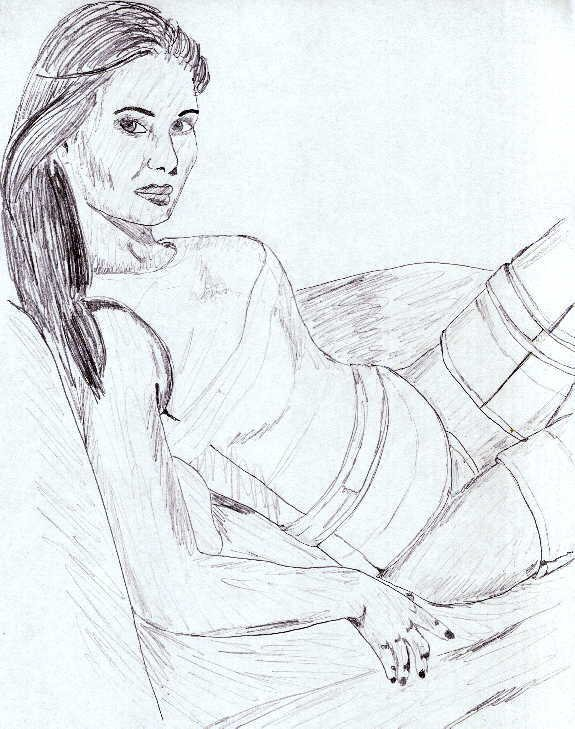
\includegraphics{images/kicks32.jpg}
\end{center}

\chapter{}

\chapter{}

\chapter{}

\chapter{}

\chapter{}

\chapter{}
\begin{thought}
Monique brought up the file on the laptop that listed the potential ``injuries.'' She then
accessed the random number generator. She hoped for something good as she instructed it to
generate a single random number between one and one hundred. She hit the ``enter'' key.
\end{thought}

``29''

\begin{thought}
She looked at the list, and found 29 on it. ``Elbow- left.'' Not bad, but not as big as she'd
hoped for.
\end{thought}

``Doctor, your patient has fractured her left elbow.''

``Well,'' I said, playing along, ``we need to get it reduced and immobilized right away. I'll
prepare the casting room.''

I headed to the bathroom and laid out the drop cloth, three inch stockinette, padding and
two and three inch plaster bandages. Monique had hobbled in after me and watched as I filled the
plastic basin with warm water.

``Good! More plaster.'' she said.

``Sure. It will match that long leg cast you already have. To be honest, that cast looks so
good, I don't want to take it off just yet.'' I sat on the edge of the tub and motioned for her
to sit on the commode.

``I don't either,'' she said as she carefully sat down. I slipped the stockinette up her arm
all the way to the shoulder, and made sure to leave some extra bunched up at the top. I made a
diagonal cut for her thumb, and then cut it off near her fingertips.

\begin{thought}
The stockinette felt great as Quinn slid it up her arm, it was smooth, soft and cool from
the air conditioned room. Monique watched intently as he made the cuts at her hand, and then
began wrapping one inch padding around her hand and wrist. When that was covered, he started at
her armpit with three inch padding, working downward. He made an extra turn at the elbow, which
she knew from experience was to pad the bones that were close to the skin.

When the padding was finished, he put on his gloves and unwrapped a roll of two inch
plaster bandage. He started at the wrist, and worked around the hand, taking care to mold the
cast well around the thumb opening and fingers. He folded back the padding and stockinette and
used another roll to anchor it, and then worked up her forearm. She knew she shouldn't move her
hand yet, but the cast looked as though she would have good movement of her thumb and fingers
when the cast was dry.

He used three inch tape to finish the cast, and he worked from the armpit downward to the
forearm. She also knew why he did this: by wrapping from the larger part of the extremity to the
smaller, it allowed each turn of the plaster to keep the previous turn from bunching up. This
kept the cast nice and smooth, as well as eliminating pressure spots inside the cast. The feel
of his hands wrapping and molding the cast, and the smell of the wet plaster were as pleasing as
watching him work.

By the time he was finished wrapping the cast, her hand and wrist were already warm from
the setting plaster. He then began buffing out the surface of the setting plaster with his hands
until it was perfectly smooth. The cast looked great- it was well formed, and thick enough to do
the job and look right, but not bulky anywhere. He also brought the cast up very high on her
arm. She couldn't tell for sure, but she wondered if it would dig in to her armpit if she
lowered her arm all the way.
\end{thought}

``Wow, it comes up really high.'' She said.

``Yes,'' I answered. We want to make sure the elbow is properly immobilized.

I held her arm for a short while longer, until I was certain that the plaster had set
enough to allow her to lower her arm. I gently lowered her arm until it rested against her body.

``How does it feel? Is it digging into your armpit?'' I asked.

``No, it actually feels great,'' Monique said. She wiggled her fingers and thumb. ``Nice
mobility of the hand, too. Excellent work, doctor!''

``Thank you, you're an outstanding patient.''

She leaned forward, and used her uncasted right arm to help herself stand up. She stepped
out of the bathroom and over near the bed. It took her a few steps to get used to balancing on
the leg cast with her arm now immobilized, too.

By this time, it was getting rather late, so we sat on the bed to watch some television
while the cast dried a bit further. Monique snuggled into me on my left, and before long, we
fell asleep.

We woke up Saturday morning still wearing our clothes from the previous day. We took turns
bathing and getting dressed. Of course, it took Monique a bit longer, and due to her casts, she
was forced to give herself a sponge bath as opposed to my hot shower. The sight of her emerging
from the bathroom, nude except for her plaster long arm and long leg casts was quite a sight to
see. I took in the view, and smiled. She would be beautiful covered in mud, but the plaster
hugging the lines of her arm and leg made her absolutely stunning.

``Hello, anyone in there?'' she asked, waving her free hand in front of my eyes.

I smiled and chuckled. ``Hey,'' I said. ``Can I help it if I find you beautiful?''

She smiled and hobbled up to me. I stood up and embraced her, my hands exploring the smooth
skin on her back. We melted into a nice long kiss, and a short time later, we found ourselves
needing to bathe again.

After we'd repeated the bathing process, she picked out clothes for the day, and I helped
her get dressed. She'd been able to undress herself, but getting dressed presented her with a
few challenges. She'd picked out a red tank top and denim shorts for the day. Once we were both
dressed, she began brushing out her hair and asked ``Where are we going today? After we eat, of
course- I'm hungry.''

``I think we'll head back to that area near the art store. It looked kind of interesting to
me. What do you think?''

``Sounds good, let's get going.''

I set up the wheelchair for her, and wheeled her out to the elevator. I used the key card
to call the elevator, and we were soon out the door and on our way. We didn't even see a single
person as we left the hotel.

We stopped at a small restaurant for a late breakfast. Most people were eating lunch by
this time, but we were still able to get a not good, but edible meal. Afterwards, we headed
across town to the Broad Ripple area. Just as it had been the day before, it looked like a
long-established area. I hesitate to say old, as everything was very well-kept. Driving through
the area looking for a parking place took a bit of time, as the traffic moved slow as there was
all manner of pedestrian traffic, and a lot of it. We saw cyclists, joggers, rollerbladers,
joggers, and people just walking around in small groups.

We found a parking place, and I started to get out the wheelchair. Monique stopped me.

``How about we just go on foot for now? If walking starts to get uncomfortable, we'll come
back for the chair.'' I agreed, and helped her out of the truck. I slung a small backpack that
I'd loaded up with art supplies over my shoulder. We headed towards a coffee shop we'd just
passed that offered outdoor seating. Monique took a seat near the sidewalk while I went in to
get our drinks.

\begin{thought}
The sun warmed Monique's face as she took in the sights. People walking, jogging, biking
and skating by. Several looked over at her, sitting there by herself. She smiled at the ones who
looked, especially the few who took a bit more than a casual glance. It didn't take too long
before it dawned on her that there seemed to be more people on bicycles and rollerblades than
she would have expected. Her arm and leg felt good in the casts. The walk from the truck to the
coffee shop had been the longest she'd walked in this leg cast, but Quinn had padded it nearly
perfectly, and she couldn't feel any hot spots from rubbing. The arm cast was heavy, and she
wondered if she might regret not having a sling before the day was over, but for now, everything
felt fine. No- better than fine. It was a beautiful day, she'd started the day off in casts,
moved on to lovemaking, and now was going out for a day in her casts with Quinn. Tonight would
probably bring another cast, and she could look forward to more of this tomorrow!
\end{thought}

``Is this seat taken?'' I asked as I returned. I handed Monique her coffee, and sat down
across from her. We sat and talked awhile, and then we got up and headed down the sidewalk,
window shopping at the small stores, going in any that caught our interest. I mentioned to
Monique that there seemed to be a lot of people on bikes and rollerblades, and they seemed to be
dressed for exercise rather than dressed just to be out. She told me that she'd had the same
thought.

As we moved Eastward along the street, many people turned to take looks at the beautiful
woman in the big casts walking along. In one of the shops, a clerk asked Monique what had
happened to her. Always thinking on her feet, she answered.

``I fell while rollerblading.''

``Wow,'' said the clerk. ``That must have been one heck of a fall!''

``Well,'' she said, ``I was moving pretty fast, and ran off the pavement. There was a hole
just off the road, and when my foot dropped into it, my leg bent just the wrong way and broke.
When I fell, I landed on my arm wrong.''

``Did it happen on the Monon?'' He asked, pointing his thumb to the East.

Monique didn't know what ``The Monon'' was, so she answered with ``No, this happened back
home, in Kentucky.

We said our goodbyes, and continued Eastward down the street. In a short time, we learned
exactly what ``The Monon'' was: It was a paved trail that had been built on an old railroad bed.
The trains that had once run through the area had been a part of the Monon line, and when the
rails were removed for the pedestrian trail, they had named it the Monon rail trail. The trail
had quite a few people on it, and we quickly learned where the cyclists and bladers had been
going- they were all headed to this trail. Many people were on bikes or on roller blades. There
were also a lot of joggers, and many people walking alone and in small groups. I turned to
Monique.

``Want to give it a try?'' I asked.

``Sure!'' she said. ``But I don't think I want to get back on my blades for a while,'' she
added with her mischievous smile.

The trail was quite beautiful. It was easy to see why so many people were using it on a
beautiful Summer Saturday. Trees lined most of the way. At the places where it crossed roads,
the intersections were well marked, and it seemed that the car traffic was very careful of the
people.

A small road ran beside the trail at one point, and we noticed a hiking shop across the
street. Monique pointed it out and suggested we go check it out, so we left the trail, and
crossed the street to the shop.

The hiking shop was a converted craftsman style home, and though it had been remodeled to
serve as a store, the quarters were cramped. The walls were covered with hiking boots and packs.
Clothes adorned a room that appeared to have once been a kitchen. A large semicircular glass
display case had been set up in what had once been the living room, and the cash register and
clerk were there. The clerk greeted us as we walked in, and took the longer than usual look at
Monique that we'd long ago learned to expect.

Monique walked over to the boots and began looking through the different styles.

``We should take a hiking trip sometime.'' She said. ``My father used to go out into the woods
to do landscapes, and I'd go with him whenever I could.''

Keeping up the charade, I replied with ``We can go as soon as you get healed up.''

Monique sighed. ``This really sucks. I hate getting hurt and having to lug these casts
around. Especially since it's summertime, and I can't do much.'' She was definitely putting on a
show for the clerk, who finally could hold her curiosity no longer.

``If you don't mind me asking, what happened to you?'' She said.

``I took a fall on my 'blades. Seeing all of these people out here on theirs sure doesn't
make me feel any better, either.'' She picked up a pair of boots. ``May I try these on? Well,
may
I try the right one on, anyway?''

``Certainly!'' the clerk relied. She pulled up a chair and handed her one of the cheap sheer
foot socks that were kept for customers who weren't wearing socks. I helped Monique ease down
into the chair, left leg sticking out in front of her. I slipped off her sandal, and helped her
get her right foot into the boot. I laced it up, and helped her to stand. She walked around the
store a bit.

``How do they feel?'' the clerk asked without thinking.

Monique didn't miss the opportunity to, once again, call attention to her casts. ``Well, the
right one feels great, but the left is a real problem,'' she said with a smile. The clerk turned
a bit red with embarrassment as she apologized. Monique turned to me.

``It feels really good. A hiking trip would be awesome, and it would be a great way to get
the strength back in my leg once I get this stupid cast off.''

I smiled at her. ``Are you saying you want the boots?''

``Yes''

I turned to the clerk. ``Ring them up, please.''

With me carrying our purchase, we left the store, and headed further up the trail. We'd
noticed a mile marker along the way, and wondered how far this trail actually went. We stopped a
guy who had been having himself a nice gawk at Monique and asked him how long the trail was. As
it turned out, it went about five miles north of where we'd entered it, and a few miles south,
as well.

We continued along the trail for another mile, and found an old iron bridge sporting a
fresh looking coat of red paint. Monique looked ready for a rest, so we sat on one of the shaded
benches at the side of the trail near the bridge. Monique scooted close to me, and I put my arm
around her. We sat for awhile without talking, as we often did. The silence was never
uncomfortable between us. After a while, she broke the silence.

``Will you really go hiking with me?'' she asked.

``Sure''

``Where should we go?'' was her next question.

``Monique, so far, I've been the one deciding where we go all the time. Since this one is
your idea, I'll let you decide where we go.''

``There's something that bothers me about that,'' she said. When I asked her what, she told
me ``I don't like making the decisions with your money. I really felt odd when I asked for the
boots''

With a scowl, I told her ``Dear God, Monique, don't worry about the stupid money!''

``I know it's not a big deal for you, but do you understand where I'm coming from? It was
just a couple months ago that I was worried about whether or not I'd be able to stay in school
full-time.''

Wow, she really is wonderful. All of my life, I've been around women who were only too
willing to spend my money, and now here was the most beautiful woman I'd ever seen, complaining
that she didn't feel right spending my money. I tried to ease her mind a bit. ``Monique, I love
you, and I love sharing what I have with you- everything. Set us up a nice trip. Don't cut
corners. If you spend too much money, I'll let you know. Other than that, don’t worry about it.
Besides, you may need to get used to spending my money.''

``What do you mean by that?'' she asked. I turned to look her dead in the eye.

``Well,'' I stumbled on the right words to say. ``Please don't freak out over what I'm going
to say. I know we've only known each other a couple of months. This thing between us is really
new, but I like it. I like it a lot. I want it to keep going.''

``I do, too,'' she replied.

``I don't want to rush anything. This is too special to me. I refuse to rush anything. But I
really do love you, Monique, and from where I sit, I can see a possibility of a day where my
money becomes our money.''

\begin{thought}
``Whoa! Did he just say what I think he said?'' Monique thought to herself. He's actually
thinking of marriage! She felt a pressure in her chest as she pondered the thought. She wondered
herself where things would end up with Quinn. It wasn't something she thought about too long at
a time, as she also knew that the relationship was very new, and while it was going great, a lot
of things could still happen. Whenever she'd had these thoughts, she'd simply reminded herself
to not get too far ahead of things, and just enjoy each day as it came.
\end{thought}

Monique had just sat there, staring at me after what I'd said. What I was starting to think
I should not have said. I HAD freaked her out, and probably done damage to our developing
relationship.

``Monique, talk to me. I just scared you, didn't I?''

``No, not at all. Well, it does scare me a bit, but not in a bad way. I'm sorry if you took
my silence as a negative response. It's just a bit overwhelming to hear you say that.''

I wasn't sure how to respond to what she'd said. She must have sensed it, because she
turned to me, stretched her casted left arm across her body, and touched my cheek with her
fingers.

``Quinn, I love you too. I love you very much. I agree we're new, and I agree that our love
has some growing to do, but I can tell you that what you're talking about is something I've
thought about, too. It's a bit overwhelming just knowing that you love me enough to think that
might be in the cards for us down the road.'' She pulled me into a kiss. I held her for a few
moments, thinking about the feelings that I had, and the way they were getting stronger. I knew
it was time to change the subject.

Softly, I said ``we just need to take things a day at a time, and never forget to enjoy
everything along the way, wherever the way takes us.''

``Agreed.'' She said with a smile. She must have also sensed that it was time to change the
subject, because she pointed to the small backpack I was wearing. ``So, is that a pencil in your
pack, or are you just happy to see me?''

I laughed and answered with ``Both!''

``I know you're the arteest, and I'm just the lowly model, but the bridge might make a nice
backdrop for a sketch,'' she said. In ten seconds, she'd taken the mood from ultra-serious to
laughing and fun. She really is great. She stepped out into the trail. She moved toward the
middle, so the other people could easily pass her, regardless of which direction they were
heading. I got out my supplies, and began working to capture her on the paper. I quickly worked
up a rough sketch, and then took out the pastels and pencils, and began to add the color.
Monique returned to the bench and watched over my shoulder as the color brought the drawing to
life. A few of the people walking by stopped briefly to watch for a bit, too. I barely noticed
them, as I was capturing the moment on paper.

By the time I'd finished, the shadows were starting to lengthen. Monique mentioned being
hungry, so we started the trek back down the trail, heading toward the truck.

\begin{thought}
Walking back down the trail, Monique's ankle was hurting just slightly inside the cast. The
cast was rubbing the ankle bone just enough to be slightly uncomfortable. Her shoulder was
starting to ache a bit from the weight of the arm cast, too. Neither was terrible, and it was
actually surprising that it hurt no more than it did, considering that she'd done a lot of
walking in the cast. She thought about mentioning it, but she was just enjoying the walk in the
afternoon sun, hand in hand with Quinn.
\end{thought}

We reached the truck, and loaded the pack, boots and other smaller purchases we'd made. I
helped her into the truck, and we headed off to dinner.

We chose another restaurant that looked somewhat busy. We put our name on the waiting list,
and grabbed a spot on a bench they'd set up for people waiting for a table. As usual, the casted
lady drew a lot of attention from patrons as the entered or left he restaurant. Our meal was
excellent, and the service was great also. We left a nice tip and headed back to the hotel. Upon
our return, I insisted that Monique let me take her upstairs in the wheelchair.

``Why?' she asked.

``You're getting another injury tonight. The chair might be our only option by bedtime. I
want it close, in case that happens. Once we were in our room, Monique decided she was going to
have another sponge bath.

``Do you need any help?'' I asked.

``No,'' she said with a smile that I didn't quite understand. She grabbed a bag and hobbled
to the bathroom as I sat down and turned on the TV, looking for something worth watching. A
short time later she emerged from the bathroom, and one look was all it took to understand the
smile that had earlier puzzled me. She was wearing a black negligee' under a black silk robe.
The black lingerie contrasted very nicely with the stark white of the plaster.

``Wow!'' was all I could say.

She smiled again. ``I know I'll soon be under the doctor's care, but first, I'd like to be
under the doctor,'' she said with a giggle.

I stood up and walked to her. We began kissing and embracing. Hands began exploring one
another, and I picked her up and carried her the few steps to the bed. I gently laid her down,
and the passion heated up from there.

When we'd finished, we lay contentedly in each other's arms for a while. We talked a bit,
but mostly we just laid there. While I loved casting her, I was totally rapt in holding her. I'm
not sure how long we were there before she pulled away, got up, and got the laptop. She opened
it, powered it up, and began tapping at the keys. When she had her result, her eyebrows raised.

``Oh my.'' She said.

\begin{center}
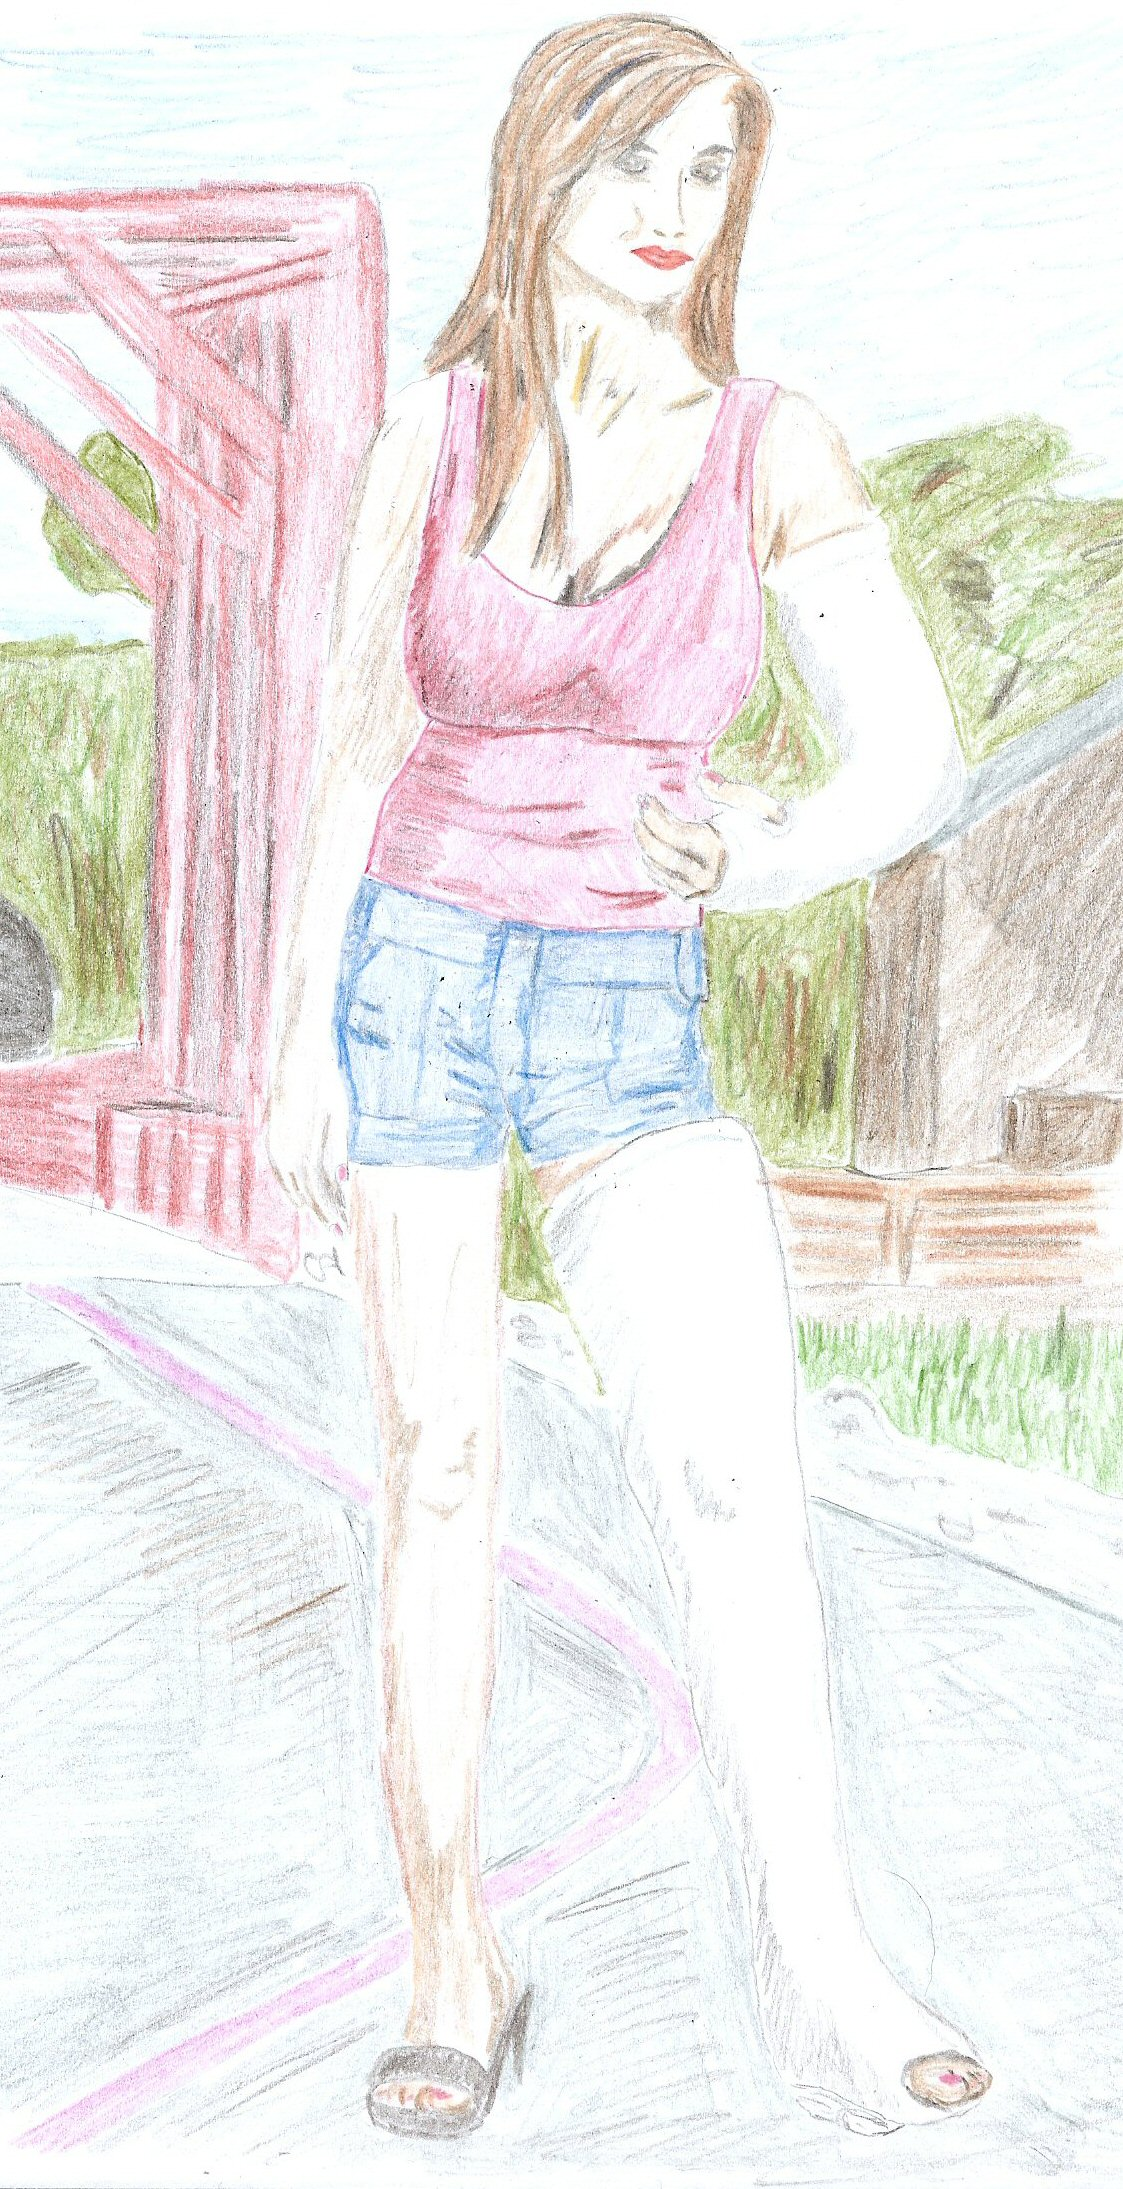
\includegraphics[height=\textheight]{images/kicks38.jpg}
\end{center}

\chapter{}

\chapter{}

\chapter{}

\chapter{}

\chapter{~}
If you've never had the pleasure of waking up next to a beautiful woman in a large,
cumbersome cast after a very passionate night, you've been missing something.

Monique was already awake, and was looking at me. I was embraced with her as well as the
situation allowed: I was mostly on my stomach, one arm underneath her back and my head resting
on her shoulder. One of my legs was over one of hers. The plaster had long lost all of its
clamminess and was completely dry.

``Good morning,'' she said with a smile, and kissed me.

I smiled back. ``Yes, it IS a good morning, and it's going to be a great day.''

``Yes it is- we'd better get moving.''

Of course, she wasn't going to be doing much moving on her own today, but I would be
happily assisting her. I had a lot to do, so I got out of bed and stretched.

``Oooohhh, you're teasing me! I'd like to stretch like that,'' she said.

``Want out of it? It can happen any time you like.''

I ducked as she threw a pillow at me with a smile.

I began getting us ready. I lifted Monique out of bed, and carried her downstairs the same
way I'd carried her up the day before. Surprisingly, going downstairs was a bit trickier than
going up. Balancing and controlling the weight of two people (plus a huge plaster cast) was a
bit challenging, but it was all a part of this great adventure. Once downstairs, I carried her
to the bathroom. I was able to get her through the door by carrying her in the upright position.
By now, with the cast completely dry, I could set her down on her feet. She had to hold herself
up with one arm, but could stand up fine. I helped her answer nature's call, and then gave her a
sponge bath. We didn't wash her hair, but that was going to be taken care of later. She wanted
to do her makeup, so I turned her around to face the mirror, and went to shower and dress
myself.

When I returned, she was nearly done, so I went ahead and prepared us a light breakfast.
Once she was finished, I helped her into the black skirt and white top she'd picked out for the
day. I then lifted her into the wheelchair, and pushed her to the kitchen, where we ate as we
talked over the plans for the day. We decided to go to Cincinnati, since that was where we'd
planned to go publicking the day of the tornado. I'd set up an appointment at a nice salon
there, where she would get a haircut and anything else she wished. I'd told them that she'd been
in an accident, and was somewhat immobile. I asked if there would be any trouble with
accessibility, and they had assured me that they would be accommodating.

Lifting her into the Expedition was as difficult as it had been the day before. Not
something I want to do very often, to be sure. The drive was uneventful, she was comfortable the
whole trip, and had no issues with carsickness, despite the distance.

Arriving at the salon, I got her into the chair and wheeled her to the door. Fortunately,
it was a double door, and as we neared the door, two stylists opened the doors to meet us.

``You must be Monique.'' One of them said as I pushed her through the door. ``My goodness, he
told us you were in a bad accident, but those casts are huge! What happened to you, anyway?''

\begin{thought}
Quinn always thinks of everything, but we'd forgotten that we'd probably get questions from
people we met. Monique thought quickly then spoke:
\end{thought}

``Well, it's actually only one cast,'' she said, lifting her shirt to show some of the
plaster over her midsection.

The girl's jaw dropped. ``Oh my God, that must be terrible! I've never seen a cast so big!
What happened to you, anyway?''

``A wall collapsed on me during the tornado that went through a couple of months ago,''
Monique said. I was impressed at her ability to make up a story so quickly, and not a lame car
crash, either- she took an event that had been big news in the entire region and made her cast a
part of it.

Mesmerized or horrified, this young lady kept asking questions as we wheeled her to the
chair. It wasn't a huge salon, and wasn't packed, but there were a few other customers there,
and they all turned to get a glance at the woman in the huge cast.

``What did you break to get a body cast like that?'' She asked as she reclined the salon
chair and turned it toward us. I lifted Monique into the chair and pushed the chair aside as I
took a seat, and enjoyed the conversation between them.

``Well, when the wall collapsed on me, it broke both of my legs between the knee and ankle,
and it also broke my left leg above the knee, and both of my hips, as well,'' Monique answered.

The girl pumped the chair up as high as it would go, but still had to crouch down a bit to
get to work on Monique's hair. She worked slowly, asking more and more questions about Monique's
``injury'' and coping with life in the cast.

\begin{thought}
This was big fun for Monique. She was the center of attention of the whole shop. She
noticed the other stylists were not having the usual small talk conversations with their
clients: everyone was listening to the conversation between her and her stylist. The questions
seemed to never end, and Monique loved answering them all: ``How long do you have to wear it?''
``Does it get hot'' ``Does it itch?'' ``My goodness, just going to the rest room has to be a
chore in
that, isn't it?'' Despite the fact that she was being somewhat nosy, Monique was very pleased
with the job she'd done washing and trimming her hair.
\end{thought}

When she'd finished with her hair, the stylist asked what else Monique would like. Monique
asked for a manicure and pedicure.

``Normally, we do those in the other room, but I'll have Jolene come to you. I'll be right
back.'' She left to get the person who does the nails, and Monique motioned me over and pulled
my
ear close to her lips.

``I think we're giving them quite the show,'' she whispered.

``Definitely,'' I responded. ``Are you having fun?''

``This is great, I'm having a ball.''

``I'm going to go get my paper and pencil. I want to capture us a memory of this.'' I smiled
and kissed her, as the stylist returned with the lady who would do Monique's nails. She was an
older lady, probably in her mid 50's. I excused myself for a moment and went and retrieved my
supplies. When I returned, the lady was still sizing up exactly how to approach the work on
Monique.

``My goodness, you have hurt yourself, haven't you?'' she looked at Monique's feet. ``Hm, we
won't be able to soak them first, but I'll do the best I can.'' She carefully washed Monique's
toes with a damp rag, and actually asked the standard generic questions as she worked.

I enjoyed watching the whole scene as Monique got the first class treatment: Monique
sneaking smiles at me, the employees and the patrons looking at the ``poor lady'' in the big
cast.
By the time she was finished with her hands, her toes were already dry, and the bright red
polish looked great contrasting with the white cast. Monique definitely chose an attention
grabbing color. While she waited for the fingernail polish to dry, I drew a quick sketch of her.

When she was ready, I lifted her back into the wheelchair, paid the bill, nicely tipped the
ladies who'd worked on her and we left. The one who had done her hair told me I was a good guy
for pampering her this way, and wished Monique a speedy recovery.

Once we were back in the truck and on the road, we laughed as we recounted the experience.
The questions, the looks, the sideways sneak looks, and the outright stares- it was all a lot
more fun than we expected it to be. One thing that stuck out on a serious note- nobody expressed
any doubts as to the cover story or the cast itself.

``We gotta go have some more fun with this thing.'' Monique said. ``Where to next?''

``Let's get something to eat.'' I answered. ``No drive through, either- someplace nice and
public.''

She agreed, and we started watching for suitable places. Soon, we found ourselves in an
interesting looking area. Though clearly in an older section of downtown, everything was clean
and well kept, and the businesses suggested that this was probably one of the trendy places.
More importantly, the sidewalks were quite busy with a lot of pedestrian traffic. Soon, we
spotted a restaurant that had a garden dining area near the street. I looked at Monique and she
nodded without a word.

I found us a parking place a couple of blocks away. I passed a couple of open spots getting
to it, but I wanted to wheel my ``badly injured'' beauty through the people walking along the
street, and we were quite the spectacle as we made our way to the café'. At least Monique was
quite the spectacle.

The outdoor dining garden was a couple of feet below street level. Fortunately, there was a
ramp. It's odd that accessibility features barely capture our notice if we have no need for
them. We see them, but they barely register in our minds. However, when you NEED them, you spot
them from quite a distance, and are very happy to see them.

As the hostess approached us, she did a slight double take at Monique, and then snapped
back to being professional. We asked for a table for two, and she led us to an open table that
had a nice view. In truth, it had two nice views: we were next to a fountain rimmed with
flowerbeds, and we were easily open to the street. Along the way to the table, I noticed people
looking at us. Some were very discreet, and a few just outright stared as we passed them. The
hostess pulled the chair out of the way so I could wheel Monique close to the table, then
stopped and turned to us.

``Will this table be alright, or would you like something more private?'' I think she was
offering us the chance to be less conspicuous. I suppose that was nice, but even if Monique were
truly injured, we wouldn't be out in such a busy area if we didn't want to be seen.

``No, this is great,'' Monique answered her. She smiled and left to send our waitress to us.

The waitress was very professional. Either Monique's cast didn't faze her, or, more likely,
the hostess had already told her about it. She took our order and left us.

While we waited for our food, we chatted. We mostly chatted quietly about some of the
people sitting nearby, and the ones walking by along the sidewalk. Most of them seemed a bit
startled when they first saw Monique, but then returned to their conversations, and paid us no
further attention.

One couple, however, was different. They were a middle aged couple. They were dressed
neatly, but casually. They were seated across the garden to my right, and Monique's left. As we
entered, we'd clearly caught their eye. While we waited, they seemed to look our way somewhat
frequently. Perhaps we were being a bit self-interested but it seemed to Monique and I that we
(or Monique, actually) had become the topic of their conversation.

By the time our food arrived, they were finishing theirs, but they stayed while we ate.
Perhaps if he'd been alone, or if they'd looked scruffy, I might have been a bit concerned. As
it was, they had an upper middle class appearance about them.

As we ate, our conversation turned to ideas for what to do with the rest of the day. We'd
discussed finding a shopping mall to ``show off'' in, but over lunch, we decided to stay in this
area and explore some of the shops in the area, and decide later if we wanted to go to a mall or
not.

``Excuse me $\ldots$'' I hadn't noticed the middle aged couple walking our way. Now, they were
at our
table, and the man was addressing us.

``I'm sorry to interrupt your lunch, but I couldn't help but notice your casts,'' he said to
Monique. He seemed slightly nervous as he asked, or maybe that was my imagination.

``I can't help but notice, either.'' Monique said with a smile. ``Hi, I'm Monique, and this is
Quinn,'' she added as she nodded my direction.

``I'm Dave,'' the man answered, smiling at Monique's remark. ``And this is my wife Molly.'' He
turned back to Monique. ``I didn't mean to stare, and I am very sorry if we bothered you. I used
to be an orthopedic technician, and leg casts attached with a spreader bar are extremely rare.
In fact, I've never seen them on an adult, except in books on the history of orthopedics.''

\newpage
\begin{center}
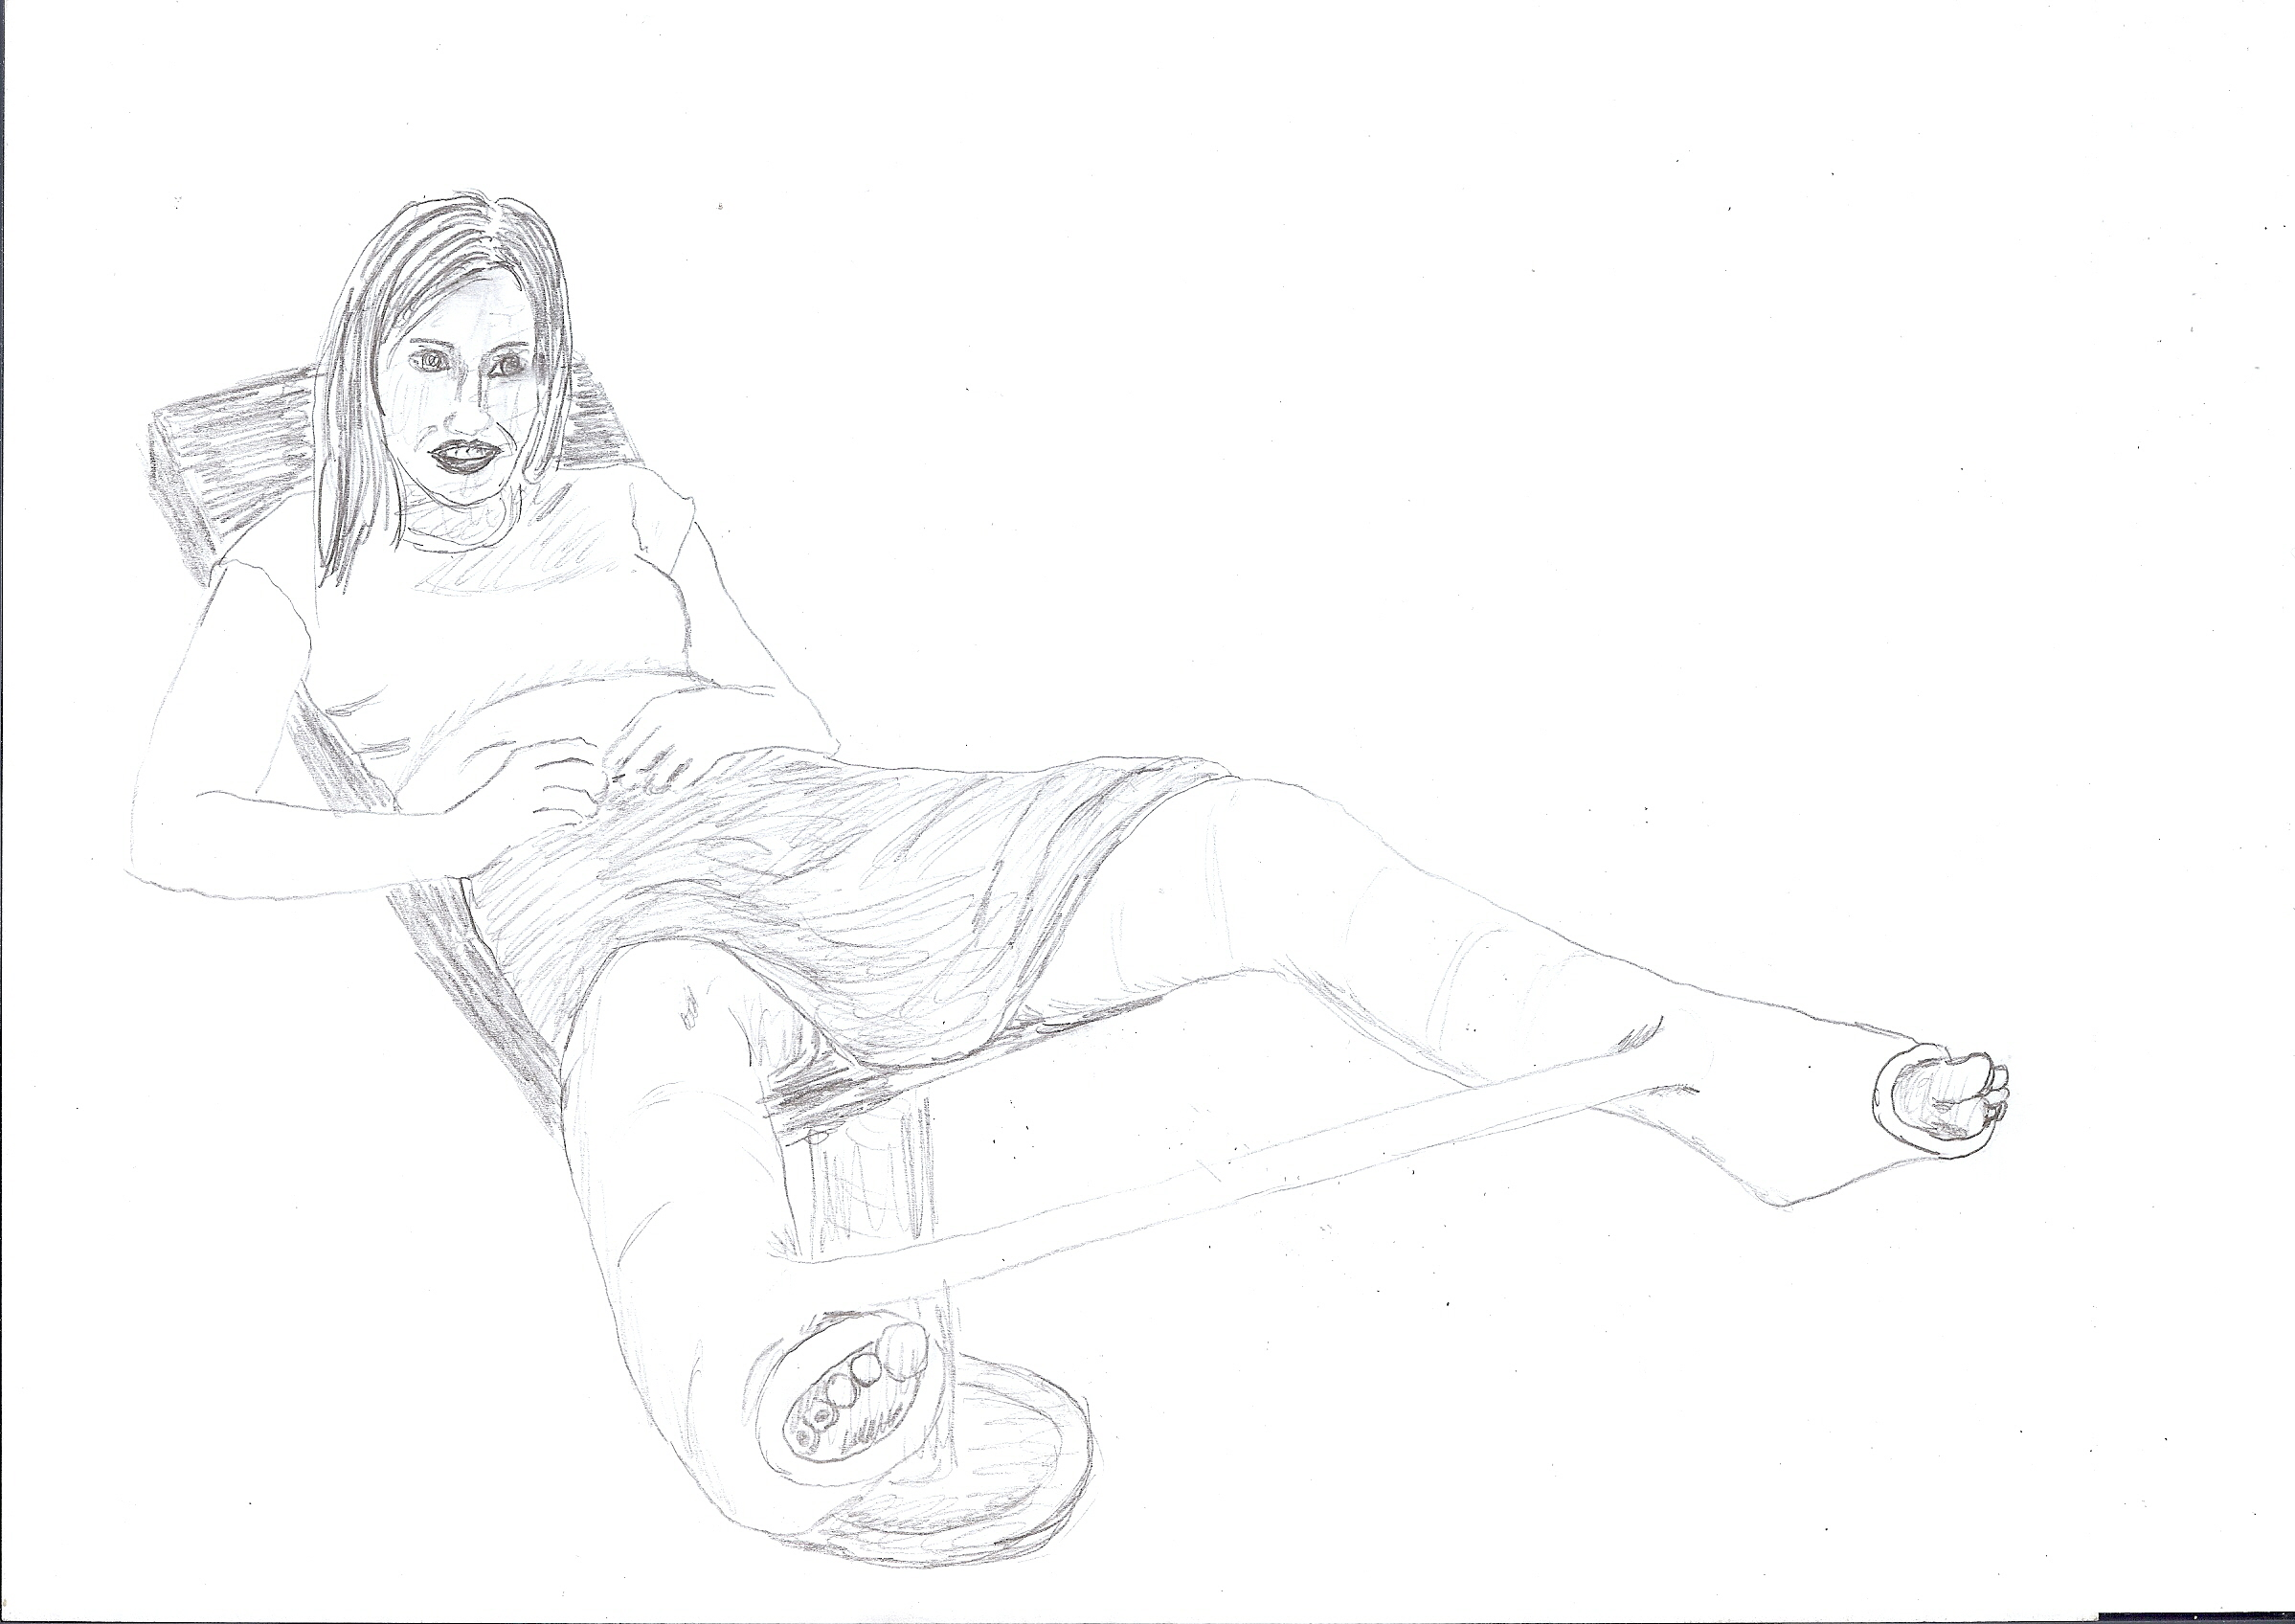
\includegraphics[width=\textwidth]{images/kicks43.jpg}
\end{center}

\chapter{}
``Excuse me…'' I hadn't noticed the middle aged couple walking our way. Now, they were at our
table, and the man was addressing us.

``I'm sorry to interrupt your lunch, but I couldn't help but notice your casts,'' he said to
Monique. He seemed slightly nervous as he asked, or maybe that was my imagination.

``I can't help but notice, either.'' Monique said with a smile. ``Hi, I'm Monique, and this is
Quinn,'' she added as she nodded my direction.

``I'm Dave,'' the man answered, smiling at Monique's remark. ``And this is my wife Molly.'' He
turned back to Monique. ``I didn't mean to stare, and I am very sorry if we bothered you. I used
to be an orthopedic technician, and leg casts attached with a spreader bar are extremely rare.
In fact, I've never seen them on an adult, except in books on the history of orthopedics.''

``This could be tricky'', I thought to myself. This guy isn't going to buy just any story.
Perhaps we should just come clean and hope they just go away shaking their heads.

\begin{thought}
``This should be fun,'' Monique thought to herself. ``Let's see if I can fool a professional.''
\end{thought}

``Actually,'' I started $\ldots$ But Monique cut me off.

``Well,'' she said. ``After the accident, they wanted to do surgery to repair the breaks, but
I begged them not to. I had a friend who slipped on ice and broke her leg. They did surgery on
her leg, and she ended up getting an infection. She spent a month in the hospital, and in the
end, she lost her leg just below the knee. I had to argue with the doctors for a day and a half
before they agreed to put me in this cast.''

``Wow!'' Dave said. ``Most doctors don't like to be second guessed. I'm surprised that he
agreed to do it. If you don't mind my curiosity, what happened to you?''

\begin{thought}
Dave seemed rather surprised at her story, but if he wasn't believing it, she couldn't
tell. Then again, she didn't know him, so she might not be able to tell.
\end{thought}

``A tornado hit my apartment building, and a wall fell on me.''

``Ouch! That's terrible! What bones did you break?''

I just sat there, watching the exchange between Dave and Monique. Molly watched, too. She
seemed a bit shy, as though she were slightly uncomfortable by the way Dave was asking questions
of a total stranger.

\begin{thought}
``Be careful, here.'' Monique thought to herself. ``At the salon, you rattled off a ridiculous
list of broken bones, and the girl ate it up. This guy won't believe just anything. Simpler is
better, here.''
\end{thought}

``I broke both of the lower leg bones on this side,'' she said, bending forward as much as
possible and pointing to her left leg. ``I broke the big bone in my lower leg on this side,''
She
said, pointing to the right. ``But the really bad part was that I broke the upper leg bone at
the
hip on this side,'' as she touched her left hip, ``and I also had a break in my pelvis, but they
said the bones hadn't moved out of place.''

``Non displaced pelvic fracture,'' Dave said.

``Yes!'' Monique said. ''That's what they called it.''

``So, you're actually in a double hip spica cast, then?''

``Yes, I knew they had a special name for it, but I'd forgotten what it was until you just
said it,'' she said.

``That's a cast that they never use on adults anymore,'' Dave said. I'm surprised that they
did it.

Monique was weaving a nice little story, and actually appeared to be deceiving a
professional. I had to chime in.

``She can be VERY enthusiastic about getting her way at times,'' I said.

``Well,'' Dave said. ``We've intruded on your time long enough. Again, I apologize for being
nosy. It's just something that I've never seen before, and my professional curiosity got the
best of me.''

``That's OK.'' Monique said. ``I get a lot of questions whenever I'm out.''

``I'll bet you do!'' He replied. ``It was nice to meet you both. You two have a great day, and
get well soon, Monique.''

``You two have a great day, too.'' I said.

As Dave and Molly walked away, they talked between themselves once they were out of
earshot. I could see them, but Monique was facing away from them.

``Do you think he believed me?'' She asked.

``I don't know, but they're talking,'' I told her. ``Either he's explaining how unlikely your
cast is, he's telling her that he thinks your story was bullshit, or he's trying to explain away
why he was talking to such a pretty gal right in front of her.''

``Honestly, from the way he looked at me, I don't think he was checking me out, just the
cast.'' She said.

``I'd like to be a fly on the wall and hear what they're saying.'' I told her. ``Medically,
your story was a stretch, but you played it well. You came off not sounding like someone knowing
a lot about orthopedics.''

We never knew it, but if we HAD heard the conversation, we'd have made a couple of new
friends that day. As they walked away, Dave said to Molly:

``I can't believe we just saw a medical DHS in public!''

``Do you think they might be casters?'' she asked.

``The cast is totally unbelievable, but she didn't sound like a caster when she talked.''

``Are we going to head back to the hotel, now? I'd like to get a nice hot soak before we get
started.''

``If you're ready to be immobilized, I'm ready to take care of you,'' he said with a smile.

``I am,'' she said with a small smile. ``But don't get any crazy ideas- I don't want another
hip spica. Not this time.''

After we finished our lunch, I paid and tipped the waitress, and I wheeled her back toward
the truck. As we walked along the sidewalk, inspiration hit me again, and I decided to do
another sketch of her. I found a spot that looked somewhat interesting that had a bench nearby.
As I sat and sketched her, Monique got more than the usual double takes and outright stares.

When I'd finished, we headed back to the truck, and along the way, we chatted about the day
so far, and what we would do next. Monique suggested that if I didn't mind an extra time
unloading and loading her, she'd like to go to a mall.

``Oh, looking for some new shoes, or a pair of jeans?'' I asked.

``Actually, I'm just looking forward to watching people react to me. We just fooled a former
orthotech. I'm feeling kind of bulletproof right now. But only if you don't mind''

``Being seen out in public with a beautiful woman in a huge cast? Uh, no- I don't mind it a
bit.'' I said, and stopped long enough to kiss her.

Going through the loading process, and then unloading once we'd found a mall that looked
big and busy was a pain. My idea for a hoist to assist in this was coming together, and I really
thought it would work. I decided that before we did another public adventure in a big cast, I'd
probably go ahead and have it built.

\begin{thought}
As they entered the mall, Monique enjoyed watching the way people reacted to her. One cast
always attracted attention, but both legs in casts, got even more. People looked a little
longer, or took an extra look over their shoulder as they walked away. Of course, they didn't
know how big the cast really was. But she did! She'd had a cramp or two in her hips, but nothing
serious. All in all, she loved the comfort and restriction of the cast. She couldn't deny that
she wasn't looking forward to getting it cut off later, but she knew that it had to end. For
now, she was just enjoying being with a great guy, and in a great cast. Then something caught
her eye.
\end{thought}

``Hey- let's stop there.'' She said, pointing to a kiosk in the middle of the walkway.

I saw the one she meant. The teenage girl working it was dressed like a flower child, and
the kiosk looked to have tie-dyed shirts, sandals, hemp jewelry and other fashion accessories
for people wanting the ``hippie'' look. As we looked, I wondered what Monique was interested in.
She'd never given me any indication that this style was anything she was interested in.

``Wanting some new sandals?'' I asked jokingly.

She played it up. ``Oh sure- now that I can't run away, you make me the butt of your jokes!''

By this time, we had the attention of the kiosk clerk.

``I'm sorry.'' I answered. ``I'm just trying to make the best of the situation.''

``Ok, I'll forgive you; on one condition,'' she said with a smile, then pointed to a small
display of sterling silver jewelry and asked the girl ``Can I see one of those toe rings?''

The girl smiled, said ``Sure!'' She took one of the rings out and said ``We have several
different styles. Let's see how this one looks. Is it OK if I put this on you?''

``Yes, please do!''

The girl was overly slow and gentle as she slipped the ring on Monique's toe. ``Is that OK?
I'm not hurting you, am I?'' she asked.

``No, no- not at all,'' Monique said, looking at her foot. ``What other styles do you have?''

I watched as she tried each one of the rings on Monique's toes. They tried several
different rings, and I have to admit, I was enjoying watching the whole thing. After the third
one, the girl asked the question. ``Sorry to be nosy, but what happened to you?''

Monique gave her the same story she'd used all day. ``I was in a tornado, and a wall fell on
me.''

``That sucks.'' The girl said, slipping on another style of toe ring. Finally, Monique
settled on a style she liked, and we got her one for each foot. I rolled her away with her new
foot jewelry in plain view.

We spent the next hour or so just walking through the mall. We didn't go into too many
shops, due to a lot of them having aisles too small. Eventually, we made our way to the food
court, and stopped to have a cup of coffee.

As we sat, we sipped coffee and chatted.

``Quinn,'' she started, ``this weekend has been a lot of fun. Everything about it has been
everything I imagined it would be.''

``Everything?'' I asked. When you were lying there shivering to death was a lot of fun?''

``Okay, that was a bit uncomfortable, but it was the only thing that was. I was totally
relaxed when you put the cast on me. Okay, I was totally relaxed physically,'' she added with a
smile. ``There were certain parts of me that were quite excited during the casting.'' I smiled
at
that.

``I don't think you know how much I've enjoyed the weekend, too.'' I told her. ``I love
putting casts on you, I love taking care of you while you're in them, I love taking you out and
showing you off in them, and then there are the other activities, too,'' I added with a raise of
my eyebrows. ``You're like no other woman I've ever known. Making love with you is always
wonderful, but when we have to find ways to work around casts, it adds an extra bit of fun.''

She went on. ``When you took me upstairs, that was amazing. I thought I was going to go
insane before you stopped. And then, I didn't think you were going to let me take care of you.''

``I was perfectly content for you not to. You can't imagine how much I enjoyed just making
you go crazy.''

Again, the smile appeared. ``And today has been a great day. I got pampered, I was the
center of attention and sympathy pretty much everywhere we went, I fooled several people,
including a cast technician that I'm actually badly hurt.''

``We THINK you fooled him. We don't know for sure,'' I corrected.

``Okay, we don't know for sure, but I bet we did. It's just been a gr…''

``Monique?'' asked a female voice from my left. We turned to see two young women in their
early twenties with shopping bags in their arms.

\begin{thought}
Monique recognized the two girls. One of them was named Angela- they'd had a few classes
together at school. The other one she knew she'd had a class with a couple of semesters ago.
They hadn't ever really talked, but she was pretty sure her name was Kaye.
\end{thought}

``Oh, Hi!'' Monique said. ``How have you guys been?''

``It looks like we've been a lot better than you!'' Angela said. ``What the hell happened to
you?''

I was stunned. I didn't know what Monique was going to say, but this was definitely a
caster's worst nightmare- being caught out in public in a cast.

\begin{thought}
From the moment she'd seen them, Monique was quickly trying to think what she was going to
say when they asked the obvious question. But, when they asked it, none of those things were
what came out. An idea flashed into her mind, and she let it out.
\end{thought}

``Did you hear about the tornado that went through right after last semester?'' Monique
asked.

``Oh no! Please don't be doing what I think you're doing.'' I thought to myself.

They both nodded. Kaye(?) said ``We all heard about that. The news said it was one of the
worst ones ever.''

The ramifications of what I already knew Monique was about to say played through my mind,
and I felt a slight twinge of panic.

Monique told her story. ``My apartment building got hit pretty hard. A wall fell on me.''

``Oh my God!'' Angie exclaimed. ``I saw that your building got hit. I was hoping you were OK.
Everyone I asked said they hadn't seen you since then. I guess I know why, now.''

``I've haven't been out too much, obviously''

``It's pretty amazing that you're out at all. My God- those casts go past your knees, and
that bar between them has to be awful!'' said Kaye(?)

``Actually,'' Monique said, reaching for the bottom of her top, ``It's all one big cast.'' She
pulled back her top just enough so that the girls could see a bit of her casted midriff. Their
jaws both fell open.

``Oh fuck! A body cast!'' Angie said. ``A body cast for summer vacation. I think I'd go
crazy!''

``Well, after lying in a hospital in traction for two weeks, I was glad to get out, even if
was with these concrete long johns. It hasn't been much fun, but I try to remind myself that
it's only temporary. As bad as it is, I remind myself that I could have been killed, or been
permanently handicapped. Not everyone was this lucky.'' (``I'm such a liar,'' she thought.
``It's
been awesome, and now it gets to be awesome for a while longer!'')

``How much longer do you have to wear it? Oh my god- classes start this week! Are you going
to have to go to class in it?'' asked Kaye(?)

``I'm going to try,'' she said. ``I'm hoping that I won't have to wear it too much longer. The
doctor has said as soon as my hip and pelvis heal, he's going to let me just have a cast on each
leg.'' Monique said. ``Hey- you two haven't met Quinn,'' she said, motioning toward me. ``He's
been
so awesome to me through all of this.''

\newpage
\begin{center}
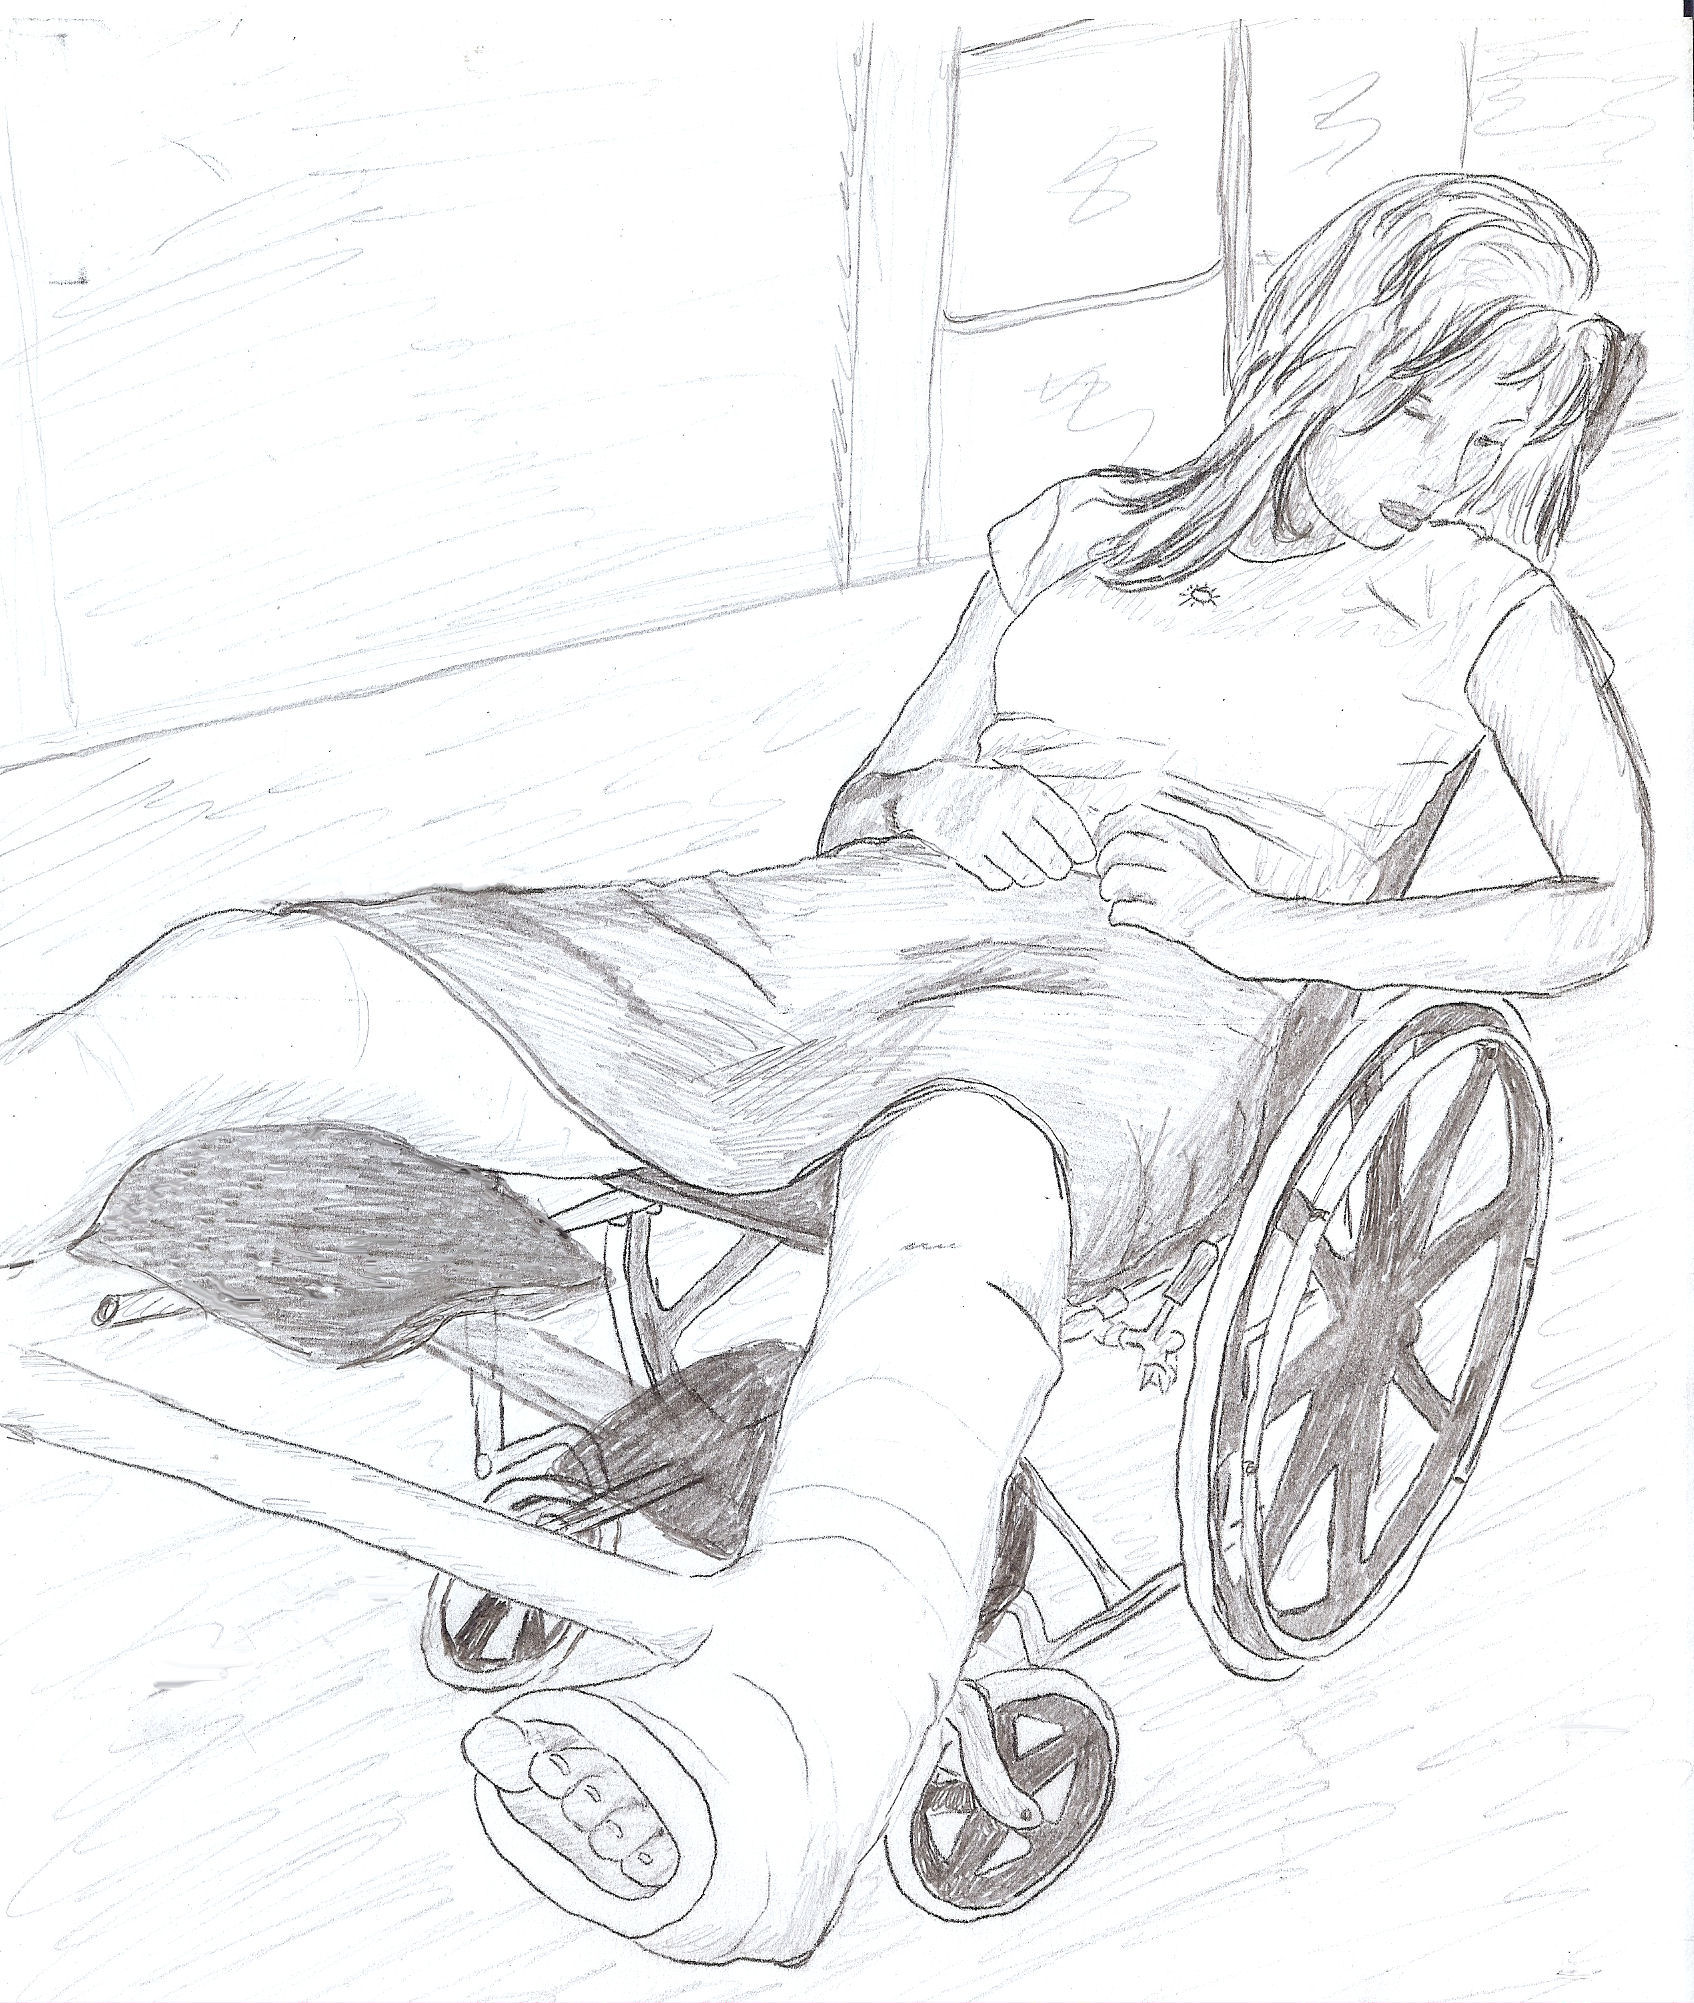
\includegraphics[width=\textwidth]{images/kicks44.jpg}
\end{center}

\chapter{~}
``You're mad, aren't you?'' Monique asked. We were on our way back home, and I hadn't said
much. I was a bit pissed at her. Weeks in a hip spica can have bad outcomes. Being with her in
that cast would be enjoyable, but my worry for her safety was overriding that.

\begin{thought}
Monique was worried. Since they'd left the mall, Quinn had been very quiet. He'd not been
receptive to her ideas about long term casts before, and now that the chance meeting had forced
them into a situation that would make a term cast the best escape, she was worried that she'd
really upset him.
\end{thought}

``A little bit. Mostly, I'm worried,'' I answered. ``I've told you before that I don't like
the idea of you wearing a term cast, but the reason I don't like it is because of the risks.
Being with you in that big cast is great. I really love it. I love taking care of you, too- I
really do.''

``Then what's the problem?''

``Well, for one, you're guaranteed to be stiff as hell when it comes off. And if you're
lucky, that's the only problem you'll have. If we're not so lucky, you can lose muscle mass in
your legs from non- use. There can be pressure sores and other skin problems. But, what scares
me the most are the possible circulatory problems- you could develop a blood clot that could
break loose and go to your brain and cause a stroke, or go to your heart or a lung and kill you
instantly.''

\begin{thought}
Monique knew about these things. She'd read about them on the internet. She'd secretly
wanted for several weeks to do a term cast, but knew Quinn would never agree to it for these
reasons. She hadn't planned to wear this one for more than the weekend, and in her desire for a
term cast hadn't really envisioned doing it in a cast this big. But, when Angie and Kaye had
bumped into them at the mall, she'd dropped into the cover story she'd been using all day
without even thinking of the ramifications initially.

When it occurred to her that the story required her to be in the cast for a while, the idea
of wearing it longer quickly became VERY appealing to her, though. She just had to convince
Quinn.
\end{thought}

``Quinn, I know about those risks. And you don't know how much I love it that you're
concerned about me. I swear that I didn't plan this. When Angie and Kaye asked about my cast, I
just started into the story without thinking about the implications.'' She said.

``Monique, I love you. There's so much about you that I never expected to find in a woman.
And I love it that you've taken to recreational casting so enthusiastically. I know you've
wanted to do a term cast, but that one is just too risky. I can't have this hurting you or
worse.''

``Let's just get home. We'll figure out what to do once we get there.'' Monique said.

Once we were home, I unloaded Monique and took her inside. She asked me to plug in her
laptop for her while I unloaded everything. While I brought in everything else, she was busily
tapping away at the keyboard. When I had everything unloaded and put away, I joined her.

``Okay, I did a bit of research,'' she started. ``I have a plan. Hear me out on this, because
it will not only work, we could have some fun with it.''

``Alright,'' I said tentatively.

``First, let's remember exactly what I said to them at the mall: I told them that I got hurt
in the tornado. That was at the end of May. That was three months ago. If I had really been
wearing a cast that long, I would be well on my way to being healed.''

``As long as the injuries weren't too severe,'' I added.

``True,'' she went on. ``But, if I remember correctly, I never even told them exactly what
sort of injuries I have.''

``Not quite. You told them something about getting two leg casts once your hip and pelvis
healed.''

``Ahh, that's right,'' she said. She thought a minute. ``But it still works. So, let's say my
injuries were a broken leg and ankle on the right, a broken leg on the left, and non displaced
breaks to the left hip and pelvis. The doctors wanted to do surgery, but I wouldn't allow it out
of fear of anesthesia, vanity over scarring, or both.''

``Monique, the story doesn't bother me- the risks to your health do!''

``Just wait. Please hear me out. I think I know how we can minimize the risks, and avoid the
embarrassment of showing up tomorrow without a cast. And have a bit more fun with this adventure
while we're at it.''

I let Monique lay out her idea without interrupting her. Her idea was to continue wearing
the plaster hip spica she was in through her first week of school. During that time, she would
mention a few times how difficult it was, lying almost flat and trying to do her school work.
Next Friday, we would cut her out of the cast, and she would spend the weekend hidden in the
house and exercising a lot. Sunday night, we would put her in a new double hip spica. She would
claim that the doctor had said she wasn't ready to be out of the big cast, but he changed it for
one in a seated position so school would be easier. The following weekend, we would again cut
her out for the weekend, and again, recast her on Sunday night, and she would pass it off as the
same cast. These seated hip spicas would be done in fiber for quicker drying.

After the 3rd week of school, we'd take her out of the DHS and put her in individual leg
casts, and she'd continue with those for a month before being out for good. In addition to
spending each weekend cast free, she would do as much exercise as possible during the week for
circulation, and she would drink green tea and take ginseng supplements to reduce the
possibility of forming clots. She said that she'd found that deep vein thrombosis was a minimal
risk for someone her age in good health, and she backed it up with research.

She'd made a good case for it. She really wanted to do it. And, to be completely honest, so
did I. With the health risks minimized, I agreed to be her partner in crime.

She held out her arms for an embrace, and I went to her and held her.

``Thank you.'' She said softly, and then added ``You know, this cast really makes me feel
sexy. And there's only one person on earth I'd want to celebrate that with. Take me upstairs?''

Monday morning, we got up early. I gave Monique a sponge bath, helped her dress, and then
propped her in front of the vanity so she could do her hair and makeup. When she was done, I
loaded her into the wheelchair and we headed for her SUV. Loading her in wasn't getting any
easier, but I'd had an idea for this. The sudden change in the situation necessitated speeding
that project along. She had a class in the morning, and one in the afternoon. While she was in
her morning class, I was going to go to a local shop and set things into motion.

When I moved her from the truck to the wheelchair, we got glances from a few people in the
parking lot. As we moved into the building, we encountered more people, and almost every one of
them, male and female, took a look at the wheelchair-bound Monique. Most of them quickly turned
back to hurrying to their classes, but a few seemed to watch a bit.

It wasn't long before we encountered someone she knew. It was a woman in her early thirties
who had shared some classes with Monique in the past. She seemed to be taken aback by the cast
quite a bit, and was very interested in hearing the story, which Monique told as though she'd
told it many times. We couldn't chat too long, as we had to get her to class.

Once in the classroom, a small crowd gathered around her to ask her questions before the
professor arrived and got things started. I made sure that her backpack with her books, laptop
and other supplies was within reach, and excused myself to go run my errand.

When I arrived at the body shop, I talked with the shop manager about the modification I
needed made to the Expedition. We worked through a few different ideas together until we came
upon a solution that we both thought would work. He quoted me a price, and I told him that I was
on a very tight schedule for needing it, and would pay a premium price if the work could be done
tomorrow. He agreed, and I wrote him a check for half of the agreed price so that he could start
gathering the materials and doing preliminary work today. I would bring the truck to him early
tomorrow, and he would do the installation. He took measurements and made notes before I left.

On my way back to get Monique, I stopped and picked us up some lunch. I retrieved her from
her class, and we went outside to the courtyard to eat. She got the usual double takes and
stares from passersby, and we once again were greeted by people she knew. One in particular
seemed to ask questions that were a bit more specific. The questions made me a bit uneasy, but
Monique handled them with ease. She'd truly gotten into the feel of playing an actual victim.
When that student left, Monique looked at me and silently mouthed the words ``Nursing student.''

The afternoon class went pretty much the same as the morning one. She got a lot of
attention and questions before class. I sat with her through this one, and helped her get
whatever she needed from her backpack, as well as helping her with a bathroom break.

\begin{thought}
The day had been a blast for Monique. She enjoyed school anyway, but fielding all of the
questions and getting so much attention had been amazing. Even when Megan, the nursing student,
had been asking the questions from a medical background, she'd enjoyed answering them. She was
confident that she'd played the victim quite well, showing only as much knowledge as someone
who'd found themselves in such a bad predicament would know.

And though it all, there had been the cast. Her legs and hips held immobile by its embrace.
Soft and comfortable on the inside, yet rigid and unyielding. And Quinn. Her love, her friend,
and now her partner in crime. She couldn't wait to get him home.
\end{thought}

Once we were home, I took Monique inside, and we discussed the day. We went over what had
been difficult, hat had been easy, and how we could deal with things better over the next few
weeks. Thankfully, Monique did not have any classes she had to attend on Tuesday, because we
both had some things that we needed to attend to: I needed to drop off the truck at the body
shop for its modifications, and we had to do some clothes shopping for Monique. She'd prepared a
skirt and some underwear to accommodate the cast, but she'd done it planning for a weekend in
the cast, not three weeks. We had to do some shopping early, so that she'd have time to do any
modifications needed. For now, she wanted to do some reading for school. Since she'd been on her
back all day, I wanted to get her on her stomach for a while to change where the pressure on her
skin was. I took her into the room with the hospital bed, and lifted her to the bed, then rolled
her onto her stomach. I left her to her reading while I prepared dinner. After we ate, I excused
myself to clean up.

\begin{thought}
Monique was feeling great about the day. Everything had been great, start to finish. Even
the challenges of eating while lying on her stomach had been fun. There was just one thing left
to make it perfect. She reached down and unclipped her skirt and untying her underwear. She
yanked the clothing from underneath herself. She then pulled off her top and bra. When Quinn
came back, she was wearing nothing but her cast and her best seductive smile. The cast prevented
them from normal lovemaking, but they'd found ways to pleasure one another around the
restrictions over the past few days, and they were getting better and better at it.
\end{thought}

Afterward, we lie together, going over our exact plans for the next day. As we did this, I
rolled her back on to her stomach and drew a sketch of her as we talked. When I'd walked into
the room after doing the dishes, her pose and expression had been so perfect that there was only
one thing I'd wanted more than to draw her. Now that we'd done that other thing, I put her back
into that position and drew her while we planned.

\newpage
\begin{center}
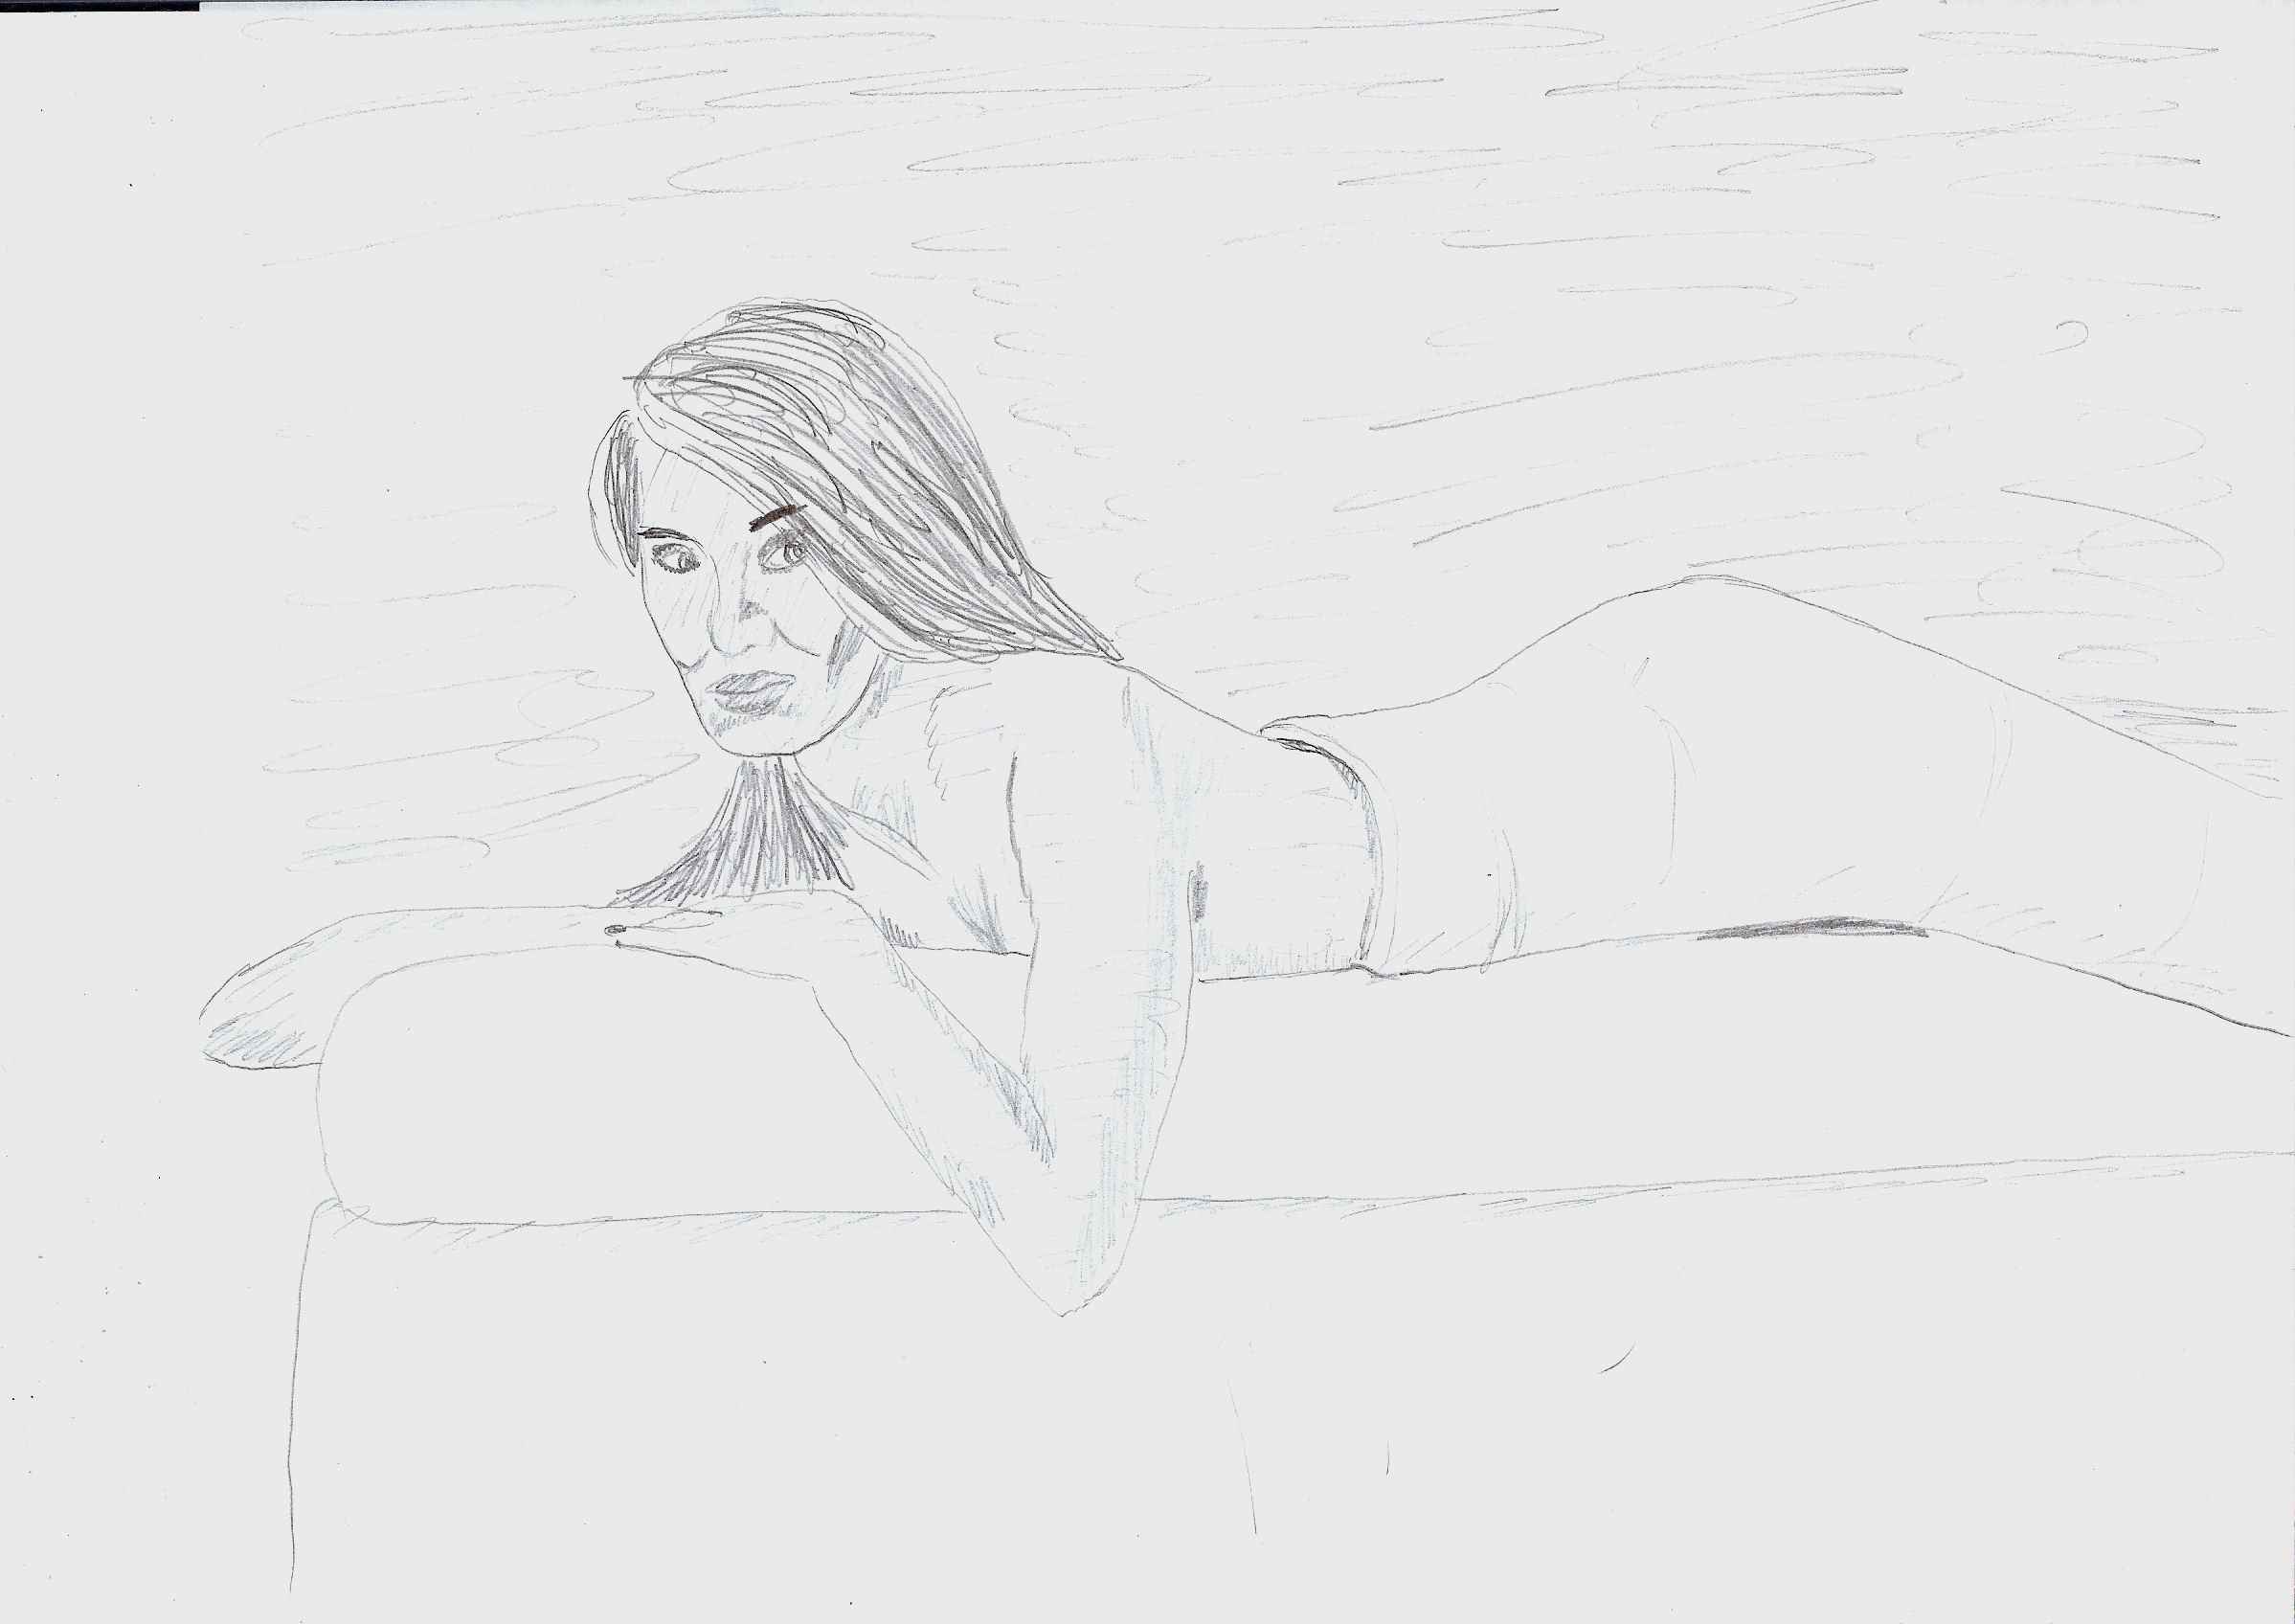
\includegraphics[width=\textwidth]{images/kicks45.jpg}
\end{center}

\chapter{}

\chapter{}

\end{document}
